\documentclass[]{book}
\usepackage{lmodern}
\usepackage{amssymb,amsmath}
\usepackage{ifxetex,ifluatex}
\usepackage{fixltx2e} % provides \textsubscript
\ifnum 0\ifxetex 1\fi\ifluatex 1\fi=0 % if pdftex
  \usepackage[T1]{fontenc}
  \usepackage[utf8]{inputenc}
\else % if luatex or xelatex
  \ifxetex
    \usepackage{mathspec}
  \else
    \usepackage{fontspec}
  \fi
  \defaultfontfeatures{Ligatures=TeX,Scale=MatchLowercase}
\fi
% use upquote if available, for straight quotes in verbatim environments
\IfFileExists{upquote.sty}{\usepackage{upquote}}{}
% use microtype if available
\IfFileExists{microtype.sty}{%
\usepackage{microtype}
\UseMicrotypeSet[protrusion]{basicmath} % disable protrusion for tt fonts
}{}
\usepackage[margin=1in]{geometry}
\usepackage{hyperref}
\hypersetup{unicode=true,
            pdftitle={Intro to Data Science for the Social Sector},
            pdfborder={0 0 0},
            breaklinks=true}
\urlstyle{same}  % don't use monospace font for urls
\usepackage{natbib}
\bibliographystyle{apalike}
\usepackage{color}
\usepackage{fancyvrb}
\newcommand{\VerbBar}{|}
\newcommand{\VERB}{\Verb[commandchars=\\\{\}]}
\DefineVerbatimEnvironment{Highlighting}{Verbatim}{commandchars=\\\{\}}
% Add ',fontsize=\small' for more characters per line
\usepackage{framed}
\definecolor{shadecolor}{RGB}{248,248,248}
\newenvironment{Shaded}{\begin{snugshade}}{\end{snugshade}}
\newcommand{\AlertTok}[1]{\textcolor[rgb]{0.94,0.16,0.16}{#1}}
\newcommand{\AnnotationTok}[1]{\textcolor[rgb]{0.56,0.35,0.01}{\textbf{\textit{#1}}}}
\newcommand{\AttributeTok}[1]{\textcolor[rgb]{0.77,0.63,0.00}{#1}}
\newcommand{\BaseNTok}[1]{\textcolor[rgb]{0.00,0.00,0.81}{#1}}
\newcommand{\BuiltInTok}[1]{#1}
\newcommand{\CharTok}[1]{\textcolor[rgb]{0.31,0.60,0.02}{#1}}
\newcommand{\CommentTok}[1]{\textcolor[rgb]{0.56,0.35,0.01}{\textit{#1}}}
\newcommand{\CommentVarTok}[1]{\textcolor[rgb]{0.56,0.35,0.01}{\textbf{\textit{#1}}}}
\newcommand{\ConstantTok}[1]{\textcolor[rgb]{0.00,0.00,0.00}{#1}}
\newcommand{\ControlFlowTok}[1]{\textcolor[rgb]{0.13,0.29,0.53}{\textbf{#1}}}
\newcommand{\DataTypeTok}[1]{\textcolor[rgb]{0.13,0.29,0.53}{#1}}
\newcommand{\DecValTok}[1]{\textcolor[rgb]{0.00,0.00,0.81}{#1}}
\newcommand{\DocumentationTok}[1]{\textcolor[rgb]{0.56,0.35,0.01}{\textbf{\textit{#1}}}}
\newcommand{\ErrorTok}[1]{\textcolor[rgb]{0.64,0.00,0.00}{\textbf{#1}}}
\newcommand{\ExtensionTok}[1]{#1}
\newcommand{\FloatTok}[1]{\textcolor[rgb]{0.00,0.00,0.81}{#1}}
\newcommand{\FunctionTok}[1]{\textcolor[rgb]{0.00,0.00,0.00}{#1}}
\newcommand{\ImportTok}[1]{#1}
\newcommand{\InformationTok}[1]{\textcolor[rgb]{0.56,0.35,0.01}{\textbf{\textit{#1}}}}
\newcommand{\KeywordTok}[1]{\textcolor[rgb]{0.13,0.29,0.53}{\textbf{#1}}}
\newcommand{\NormalTok}[1]{#1}
\newcommand{\OperatorTok}[1]{\textcolor[rgb]{0.81,0.36,0.00}{\textbf{#1}}}
\newcommand{\OtherTok}[1]{\textcolor[rgb]{0.56,0.35,0.01}{#1}}
\newcommand{\PreprocessorTok}[1]{\textcolor[rgb]{0.56,0.35,0.01}{\textit{#1}}}
\newcommand{\RegionMarkerTok}[1]{#1}
\newcommand{\SpecialCharTok}[1]{\textcolor[rgb]{0.00,0.00,0.00}{#1}}
\newcommand{\SpecialStringTok}[1]{\textcolor[rgb]{0.31,0.60,0.02}{#1}}
\newcommand{\StringTok}[1]{\textcolor[rgb]{0.31,0.60,0.02}{#1}}
\newcommand{\VariableTok}[1]{\textcolor[rgb]{0.00,0.00,0.00}{#1}}
\newcommand{\VerbatimStringTok}[1]{\textcolor[rgb]{0.31,0.60,0.02}{#1}}
\newcommand{\WarningTok}[1]{\textcolor[rgb]{0.56,0.35,0.01}{\textbf{\textit{#1}}}}
\usepackage{longtable,booktabs}
\usepackage{graphicx,grffile}
\makeatletter
\def\maxwidth{\ifdim\Gin@nat@width>\linewidth\linewidth\else\Gin@nat@width\fi}
\def\maxheight{\ifdim\Gin@nat@height>\textheight\textheight\else\Gin@nat@height\fi}
\makeatother
% Scale images if necessary, so that they will not overflow the page
% margins by default, and it is still possible to overwrite the defaults
% using explicit options in \includegraphics[width, height, ...]{}
\setkeys{Gin}{width=\maxwidth,height=\maxheight,keepaspectratio}
\IfFileExists{parskip.sty}{%
\usepackage{parskip}
}{% else
\setlength{\parindent}{0pt}
\setlength{\parskip}{6pt plus 2pt minus 1pt}
}
\setlength{\emergencystretch}{3em}  % prevent overfull lines
\providecommand{\tightlist}{%
  \setlength{\itemsep}{0pt}\setlength{\parskip}{0pt}}
\setcounter{secnumdepth}{5}
% Redefines (sub)paragraphs to behave more like sections
\ifx\paragraph\undefined\else
\let\oldparagraph\paragraph
\renewcommand{\paragraph}[1]{\oldparagraph{#1}\mbox{}}
\fi
\ifx\subparagraph\undefined\else
\let\oldsubparagraph\subparagraph
\renewcommand{\subparagraph}[1]{\oldsubparagraph{#1}\mbox{}}
\fi

%%% Use protect on footnotes to avoid problems with footnotes in titles
\let\rmarkdownfootnote\footnote%
\def\footnote{\protect\rmarkdownfootnote}

%%% Change title format to be more compact
\usepackage{titling}

% Create subtitle command for use in maketitle
\newcommand{\subtitle}[1]{
  \posttitle{
    \begin{center}\large#1\end{center}
    }
}

\setlength{\droptitle}{-2em}

  \title{Intro to Data Science for the Social Sector}
    \pretitle{\vspace{\droptitle}\centering\huge}
  \posttitle{\par}
    \author{}
    \preauthor{}\postauthor{}
      \predate{\centering\large\emph}
  \postdate{\par}
    \date{Updated August 29, 2018}

\usepackage{booktabs}
\usepackage{amsthm}
\makeatletter
\def\thm@space@setup{%
  \thm@preskip=8pt plus 2pt minus 4pt
  \thm@postskip=\thm@preskip
}
\makeatother

\usepackage{amsthm}
\newtheorem{theorem}{Theorem}[chapter]
\newtheorem{lemma}{Lemma}[chapter]
\theoremstyle{definition}
\newtheorem{definition}{Definition}[chapter]
\newtheorem{corollary}{Corollary}[chapter]
\newtheorem{proposition}{Proposition}[chapter]
\theoremstyle{definition}
\newtheorem{example}{Example}[chapter]
\theoremstyle{definition}
\newtheorem{exercise}{Exercise}[chapter]
\theoremstyle{remark}
\newtheorem*{remark}{Remark}
\newtheorem*{solution}{Solution}
\begin{document}
\maketitle

{
\setcounter{tocdepth}{1}
\tableofcontents
}
\hypertarget{welcome}{%
\chapter*{Welcome}\label{welcome}}
\addcontentsline{toc}{chapter}{Welcome}

Welcome to the course text for Data Science for the Social Sector.

This course introduces students to the field of data science and its
applications in the public sector. Modern performance management and
evaluation processes require strong data literacy and the ability to
combine and analyze data from a variety of sources to inform managerial
processes. We offer a practical, tools-based approach that is designed
to build strong foundations for people that want to work as policy
analysts or data-driven managers. We will cover data programming
fundamentals, visualization, text analysis, automated reporting, and
dynamic reporting using dashboards. The course is analytically rigorous,
but no prior programming experience is assumed.

\textbf{The Data Science Process (Wickham \& Grolemund, 2016):}

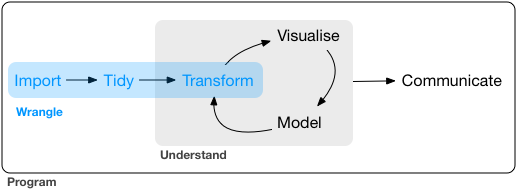
\includegraphics{figures/data-science-wrangle.png}

\begin{quote}
\emph{A data scientist is a person who should be able to leverage
existing data sources, and create new ones as needed in order to extract
meaningful information and actionable insights. These insights can be
used to drive business decisions and changes intended to achieve
business goals\ldots{} `The Perfect Data Scientist' is the individual
who is equally strong in business, programming, statistics, and
communication.}
\end{quote}

From:
\href{https://www.innoarchitech.com/what-is-data-science-does-data-scientist-do/}{``What
Is Data Science, and What Does a Data Scientist Do?''}

\hypertarget{part-part-i-foundations}{%
\part{PART I: FOUNDATIONS}\label{part-part-i-foundations}}

\hypertarget{introduction-to-r}{%
\chapter{Introduction to R}\label{introduction-to-r}}

This lecture introduces you to basic operations when you first start
using R such as navigation, the object-oriented framework, loading a
package, and creating some data vectors.

\hypertarget{navigation}{%
\section{Navigation}\label{navigation}}

You need to know a few operations to help you maneuver the R work
environment, such as listing objects (datasets and functions) that are
active, changing your working directory, listing available files, and
finding help.

\hypertarget{setting-your-working-directory}{%
\subsection{Setting Your Working
Directory}\label{setting-your-working-directory}}

When you are ready to load data, R needs to know where to look for your
files. You can check what is avaiable in the current directory
(i.e.~folder) by asking to list all of the current files using
\textbf{dir()}.

\begin{Shaded}
\begin{Highlighting}[]
\KeywordTok{dir}\NormalTok{()}
\end{Highlighting}
\end{Shaded}

If the file that you need is located in a different folder, you can
change directories easily in R Studio by Session -\textgreater{} Set
working director -\textgreater{} Choose directory (or Ctrl + Shift + H).

If you are writing a script, you want to keep track of this step so that
it can be reproduced. Use the function \textbf{get.wd()} to check your
current working directory, and \textbf{set.wd()} to change. You need to
specify your path as an argument to this function, such as.

\begin{Shaded}
\begin{Highlighting}[]
\KeywordTok{setwd}\NormalTok{( }\StringTok{"C:/user/projects/financial model"}\NormalTok{ )}
\end{Highlighting}
\end{Shaded}

NOTE! R uses unix style notation with forward slashes, so if you copy
and paste from Windows it will look like this, with back slashes:

\begin{Shaded}
\begin{Highlighting}[]
\KeywordTok{setwd}\NormalTok{( }\StringTok{"C:\textbackslash{}user\textbackslash{}projects}\CharTok{\textbackslash{}f}\StringTok{inancial model"}\NormalTok{ )}
\end{Highlighting}
\end{Shaded}

You will need to change them around for it to work.

It is best to save all of your steps in your scripts so that the
analysis can be reproduced by yourself or others. In some cases you are
doing exploratory or summary work, and you may want to find a file a
quickly. You can use the \textbf{file.choose()} function to open a GUI
to select your file directly. This function is used as an argument
inside of a load data function.

\begin{Shaded}
\begin{Highlighting}[]
\NormalTok{my.dat <-}\StringTok{ }\KeywordTok{read.csv}\NormalTok{( }\KeywordTok{file.choose}\NormalTok{() )}
\end{Highlighting}
\end{Shaded}

\hypertarget{commenting-code}{%
\section{Commenting Code}\label{commenting-code}}

Most computer languages have a special character that is used to
``comment out'' lines so that it is not run by the program. It is used
for two important purposes. First, we can add text to document our
functions and it will not interfere with the program. And two, we can
use it to run a program while ignoring some of the code, often for
debugging purposes.

The \textbf{\#} hash tag is used for comments in R.

\begin{Shaded}
\begin{Highlighting}[]

\CommentTok{##==============================================}
\CommentTok{##}
\CommentTok{##  Here is some documentation for this script}
\CommentTok{##}
\CommentTok{##==============================================}

\NormalTok{x <-}\StringTok{ }\DecValTok{1}\OperatorTok{:}\DecValTok{10}

\KeywordTok{sum}\NormalTok{( x )}
\CommentTok{### [1] 55}

\CommentTok{# y <- 1:25     # not run}

\CommentTok{# sum( y )      # not run}
\end{Highlighting}
\end{Shaded}

\hypertarget{help}{%
\section{Help}\label{help}}

You will use the help functions frequently to figure out what arguments
and values are needed for specific functions. Because R is very
customizable, you will find that many functions have several or dozens
of arguments, and it is difficult to remember the correct syntax and
values. But don't worry, to look them up all you need is the function
name and a call for help:

\begin{quote}
help( dotchart ) \# opens an external helpfile
\end{quote}

If you just need to remind yourself which arguments are defined in a
function, you can use the \emph{args()} command:

\begin{Shaded}
\begin{Highlighting}[]
\KeywordTok{args}\NormalTok{( dotchart )}
\CommentTok{### function (x, labels = NULL, groups = NULL, gdata = NULL, cex = par("cex"), }
\CommentTok{###     pt.cex = cex, pch = 21, gpch = 21, bg = par("bg"), color = par("fg"), }
\CommentTok{###     gcolor = par("fg"), lcolor = "gray", xlim = range(x[is.finite(x)]), }
\CommentTok{###     main = NULL, xlab = NULL, ylab = NULL, ...) }
\CommentTok{### NULL}
\end{Highlighting}
\end{Shaded}

If you can't recall a function name, you can list all of the functions
from a specific package as follows:

\begin{quote}
help( package=``stats'' ) \# lists all functions in stats package
\end{quote}

\hypertarget{install-programs-packages}{%
\section{Install Programs (packages)}\label{install-programs-packages}}

When you open R by default it will launch a core set of programs, called
``packages'' in R speak, that are use for most data operations. To see
which packages are currently active use the \textbf{search()} function.

\begin{Shaded}
\begin{Highlighting}[]
\KeywordTok{search}\NormalTok{()}
\CommentTok{###  [1] ".GlobalEnv"        "package:bindrcpp"  "package:ggplot2"  }
\CommentTok{###  [4] "package:scales"    "package:reshape2"  "package:tidyr"    }
\CommentTok{###  [7] "package:maps"      "package:Lahman"    "package:pander"   }
\CommentTok{### [10] "package:dplyr"     "package:bookdown"  "package:rmarkdown"}
\CommentTok{### [13] "package:stats"     "package:graphics"  "package:grDevices"}
\CommentTok{### [16] "package:utils"     "package:datasets"  "package:methods"  }
\CommentTok{### [19] "Autoloads"         "package:base"}
\end{Highlighting}
\end{Shaded}

These programs manage the basic data operations, run the core graphics
engine, and give you basic statistical methods.

The real magic for R comes from the over 7,000 contributed packages
available on the CRAN: \url{https://cran.r-project.org/web/views/}

A package consists of custom functions and datasets that are generated
by users. They are \emph{packaged} together so that they can be shared
with others. A package also includes documentation that describes each
function, defines all of the arguments, and documents any datasets that
are included.

If you know a package name, it is easy to install. In R Studio you can
select Tools -\textgreater{} Install Packages and a list of available
packages will be generated. But it is easier to use the
\textbf{install.packages()} command. We will use the Lahman Package in
this course, so let's install that now.

\textbf{Description} \emph{This package provides the tables from Sean
Lahman's Baseball Database as a set of R data.frames. It uses the data
on pitching, hitting and fielding performance and other tables from 1871
through 2013, as recorded in the 2014 version of the database.}

See the documentation here:
\url{https://cran.r-project.org/web/packages/Lahman/Lahman.pdf}

\begin{Shaded}
\begin{Highlighting}[]

\KeywordTok{install.packages}\NormalTok{( }\StringTok{"Lahman"}\NormalTok{ )}
\end{Highlighting}
\end{Shaded}

You will be asked to select a ``mirror''. In R speak this just means the
server from which you will download the package (choose anything
nearby). R is a community of developers and universities that create
code and maintain the infrastructure. A couple of dozen universities
around the world host servers that contain copies of the R packages so
that they can be easily accessed everywhere.

If the package is successfully installed you will get a message similar
to this:

\begin{quote}
package `Lahman' successfully unpacked and MD5 sums checked
\end{quote}

Once a new program is installed you can now open (``load'' in R speak)
the package using the \textbf{library()} command:

\begin{Shaded}
\begin{Highlighting}[]
\KeywordTok{library}\NormalTok{( }\StringTok{"Lahman"}\NormalTok{ )}
\end{Highlighting}
\end{Shaded}

If you now type \textbf{search()} you can see that Lahman has been added
to the list of active programs. We can now access all of the functions
and data that are available in the Lahman package.

\hypertarget{accessing-built-in-datasets-in-r}{%
\section{Accessing Built-In Datasets in
R}\label{accessing-built-in-datasets-in-r}}

One nice feature of R is that is comes with a bunch of built-in datasets
that have been contributed by users are are loaded automatically. You
can see the list of available datasets by typing:

\begin{Shaded}
\begin{Highlighting}[]
\KeywordTok{data}\NormalTok{()}
\end{Highlighting}
\end{Shaded}

This will list all of the default datasets in core R packages. If you
want to see all of the datasets available in installed packages as well
use:

\begin{Shaded}
\begin{Highlighting}[]
\KeywordTok{data}\NormalTok{( }\DataTypeTok{package =} \KeywordTok{.packages}\NormalTok{(}\DataTypeTok{all.available =} \OtherTok{TRUE}\NormalTok{) )}
\end{Highlighting}
\end{Shaded}

\hypertarget{basic-data-operations}{%
\subsection{Basic Data Operations}\label{basic-data-operations}}

Let's ignore the underlying data structure right now and look at some
ways that we might interact with data.

We will use the \textbf{USArrests} dataset available in the core files.

To access the data we need to load it into working memory. Anything that
is active in R will be listed in the environment, which you can check
using the \textbf{ls()} command. We will load the dataset using the
\textbf{data()} command.

\begin{Shaded}
\begin{Highlighting}[]
\KeywordTok{remove}\NormalTok{( }\DataTypeTok{list=}\KeywordTok{ls}\NormalTok{() )}
\end{Highlighting}
\end{Shaded}

\begin{Shaded}
\begin{Highlighting}[]

\KeywordTok{ls}\NormalTok{() }\CommentTok{# nothing currently available}
\CommentTok{### character(0)}

\KeywordTok{data}\NormalTok{( }\StringTok{"USArrests"}\NormalTok{ )}

\KeywordTok{ls}\NormalTok{() }\CommentTok{# data is now avaible for use}
\CommentTok{### [1] "USArrests"}
\end{Highlighting}
\end{Shaded}

Now that we have loaded a dataset, we can start to access the variables
and analyze relationships. Let's get to know our dataset.

\begin{Shaded}
\begin{Highlighting}[]

\KeywordTok{names}\NormalTok{( USArrests )  }\CommentTok{# what variables are in the dataset?}
\CommentTok{### [1] "Murder"   "Assault"  "UrbanPop" "Rape"}

\KeywordTok{nrow}\NormalTok{( USArrests )   }\CommentTok{# how many observations are there?}
\CommentTok{### [1] 50}

\KeywordTok{dim}\NormalTok{( USArrests )    }\CommentTok{# a quick way to see rows and columns - the dimensions of the dataset}
\CommentTok{### [1] 50  4}

\KeywordTok{row.names}\NormalTok{( }\KeywordTok{head}\NormalTok{( USArrests ) )   }\CommentTok{# what are the obsevations (rows) in our data}
\CommentTok{### [1] "Alabama"    "Alaska"     "Arizona"    "Arkansas"   "California"}
\CommentTok{### [6] "Colorado"}

\KeywordTok{summary}\NormalTok{( USArrests )   }\CommentTok{# summary statistics of variables}
\CommentTok{###      Murder          Assault         UrbanPop          Rape      }
\CommentTok{###  Min.   : 0.800   Min.   : 45.0   Min.   :32.00   Min.   : 7.30  }
\CommentTok{###  1st Qu.: 4.075   1st Qu.:109.0   1st Qu.:54.50   1st Qu.:15.07  }
\CommentTok{###  Median : 7.250   Median :159.0   Median :66.00   Median :20.10  }
\CommentTok{###  Mean   : 7.788   Mean   :170.8   Mean   :65.54   Mean   :21.23  }
\CommentTok{###  3rd Qu.:11.250   3rd Qu.:249.0   3rd Qu.:77.75   3rd Qu.:26.18  }
\CommentTok{###  Max.   :17.400   Max.   :337.0   Max.   :91.00   Max.   :46.00}
\end{Highlighting}
\end{Shaded}

We can see that the dataset consists of four variables: Murder, Assault,
UrbanPop, and Rape. We also see that our unit of analysis is the state.
But where does the data come from, and how are these variables measured?

To see the documentation for a specific dataset you will need to use the
\textbf{help()} function:

\begin{Shaded}
\begin{Highlighting}[]
\KeywordTok{help}\NormalTok{( }\StringTok{"USArrests"}\NormalTok{ )}
\end{Highlighting}
\end{Shaded}

We get valuable information about the source and metrics:

\textbf{Description} \emph{This data set contains statistics, in arrests
per 100,000 residents for assault, murder, and rape in each of the 50 US
states in 1973. Also given is the percent of the population living in
urban areas.}

\textbf{Format} \emph{A data frame with 50 observations on 4 variables.}

\begin{itemize}
\tightlist
\item
  \textbf{Murder}: numeric Murder arrests (per 100,000)
\item
  \textbf{Assault}: numeric Assault arrests (per 100,000)
\item
  \textbf{UrbanPop}: numeric Percent urban population
\item
  \textbf{Rape}: numeric Rape arrests (per 100,000)
\end{itemize}

To access a specific variable inside of a dataset, you will use the
\emph{\$} operator between the dataset name and the variable name:

\begin{Shaded}
\begin{Highlighting}[]

\KeywordTok{summary}\NormalTok{( USArrests}\OperatorTok{$}\NormalTok{Murder )}
\CommentTok{###    Min. 1st Qu.  Median    Mean 3rd Qu.    Max. }
\CommentTok{###   0.800   4.075   7.250   7.788  11.250  17.400}
\KeywordTok{summary}\NormalTok{( USArrests}\OperatorTok{$}\NormalTok{Assault )}
\CommentTok{###    Min. 1st Qu.  Median    Mean 3rd Qu.    Max. }
\CommentTok{###    45.0   109.0   159.0   170.8   249.0   337.0}

\CommentTok{# Is there a relationship between urban density and crime?}

\KeywordTok{plot}\NormalTok{( USArrests}\OperatorTok{$}\NormalTok{UrbanPop, USArrests}\OperatorTok{$}\NormalTok{Murder )}
\KeywordTok{abline}\NormalTok{( }\KeywordTok{lm}\NormalTok{( USArrests}\OperatorTok{$}\NormalTok{Murder }\OperatorTok{~}\StringTok{ }\NormalTok{USArrests}\OperatorTok{$}\NormalTok{UrbanPop ), }\DataTypeTok{col=}\StringTok{"red"}\NormalTok{ )}
\end{Highlighting}
\end{Shaded}

\begin{center}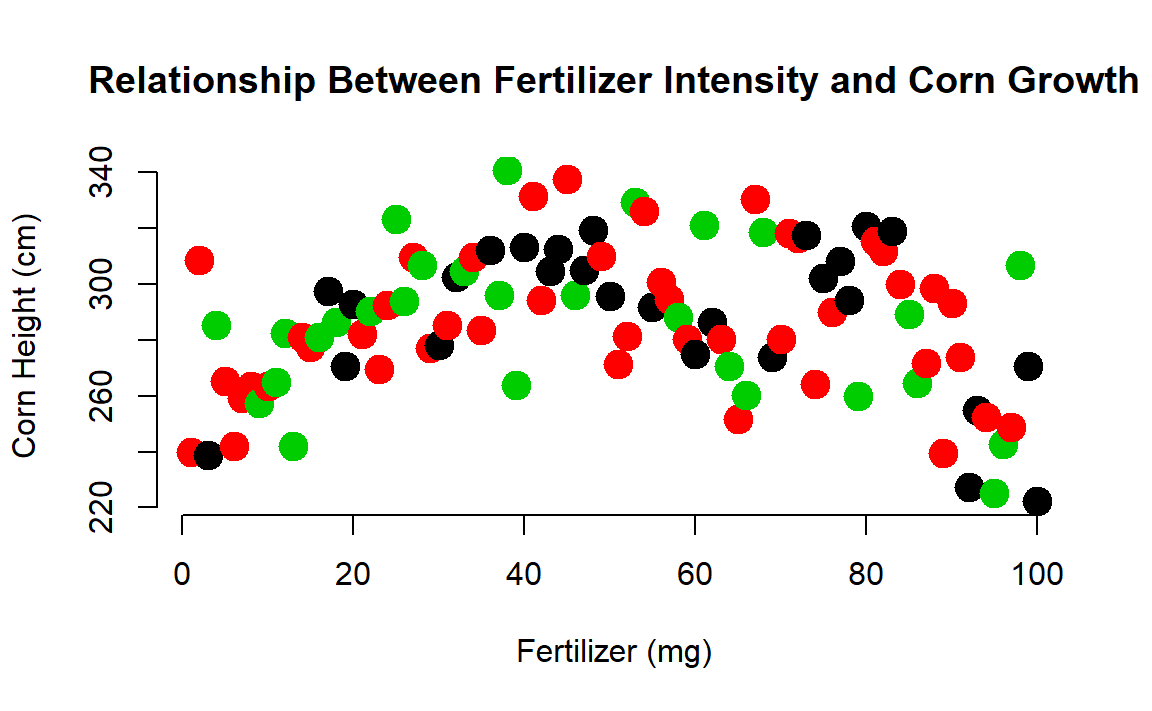
\includegraphics[width=0.7\linewidth]{DS4PS-I_files/figure-latex/unnamed-chunk-19-1} \end{center}

\hypertarget{using-the-lahman-data}{%
\subsection{Using the Lahman Data}\label{using-the-lahman-data}}

Let's take a look at some of the data available in the Lahman package.

\begin{Shaded}
\begin{Highlighting}[]

\KeywordTok{data}\NormalTok{( }\DataTypeTok{package =} \StringTok{"Lahman"}\NormalTok{ ) }\CommentTok{# All datasets in package ‘Lahman’:}
\end{Highlighting}
\end{Shaded}

\begin{longtable}[]{@{}ll@{}}
\toprule
TABLE NAME & DEFITION\tabularnewline
\midrule
\endhead
AllstarFull & AllstarFull table\tabularnewline
Appearances & Appearances table\tabularnewline
AwardsManagers & AwardsManagers table\tabularnewline
AwardsPlayers & AwardsPlayers table\tabularnewline
AwardsShareManagers & AwardsShareManagers table\tabularnewline
AwardsSharePlayers & AwardsSharePlayers table\tabularnewline
Batting & Batting table\tabularnewline
BattingPost & BattingPost table\tabularnewline
CollegePlaying & CollegePlaying table\tabularnewline
Fielding & Fielding table\tabularnewline
FieldingOF & FieldingOF table\tabularnewline
FieldingPost & FieldingPost data\tabularnewline
HallOfFame & Hall of Fame Voting Data\tabularnewline
LahmanData & Lahman Datasets\tabularnewline
Managers & Managers table\tabularnewline
ManagersHalf & ManagersHalf table\tabularnewline
Master & Master table\tabularnewline
Pitching & Pitching table\tabularnewline
PitchingPost & PitchingPost table\tabularnewline
Salaries & Salaries table\tabularnewline
Schools & Schools table\tabularnewline
SeriesPost & SeriesPost table\tabularnewline
Teams & Teams table\tabularnewline
TeamsFranchises & TeamFranchises table\tabularnewline
TeamsHalf & TeamsHalf table\tabularnewline
battingLabels & Variable Labels\tabularnewline
fieldingLabels & Variable Labels\tabularnewline
pitchingLabels & Variable Labels\tabularnewline
\bottomrule
\end{longtable}

We see that we have lots of datasets to choose from here. I will use the
Master dataset, which is a list of all of the Major League Baseball
players over the past century, and their personal information.

\begin{Shaded}
\begin{Highlighting}[]

\KeywordTok{library}\NormalTok{( Lahman )    }\CommentTok{# loads Lahman package}
\KeywordTok{data}\NormalTok{( Master )}
\KeywordTok{head}\NormalTok{( Master ) }
\end{Highlighting}
\end{Shaded}

Here are some common functions for exploring datasets:

\begin{Shaded}
\begin{Highlighting}[]
\KeywordTok{names}\NormalTok{( Master )      }\CommentTok{# variable names}
\KeywordTok{nrow}\NormalTok{( Master )       }\CommentTok{# 18,354 players included}
\KeywordTok{summary}\NormalTok{( Master )    }\CommentTok{# descriptive statistics of variables}
\end{Highlighting}
\end{Shaded}

We can use \textbf{help(Master)} to get information about the dataset,
including a data dictionary.

\begin{Shaded}
\begin{Highlighting}[]

\KeywordTok{help}\NormalTok{( Master )}
\end{Highlighting}
\end{Shaded}

\textbf{MASTER TABLE}

\begin{center}\rule{0.5\linewidth}{\linethickness}\end{center}

\textbf{Description}

Master table - Player names, DOB, and biographical info. This file is to
be used to get details about players listed in the Batting, Pitching,
and other files where players are identified only by playerID.

\textbf{Usage}

data(Master)

\textbf{Format}

A data frame with 19105 observations on the following 26 variables.

\begin{itemize}
\tightlist
\item
  \textbf{playerID}: A unique code asssigned to each player. The
  playerID links the data in this file with records on players in the
  other files.
\item
  \textbf{birthYear}: Year player was born
\item
  \textbf{birthMonth}: Month player was born
\item
  \textbf{birthDay}: Day player was born
\item
  \textbf{birthCountry}: Country where player was born
\item
  \textbf{birthState}: State where player was born
\item
  \textbf{birthCity}: City where player was born
\item
  \textbf{deathYear}: Year player died
\item
  \textbf{deathMonth}: Month player died
\item
  \textbf{deathDay}: Day player died
\item
  \textbf{deathCountry}: Country where player died
\item
  \textbf{deathState}: State where player died
\item
  \textbf{deathCity}: City where player died
\item
  \textbf{nameFirst}: Player's first name
\item
  \textbf{nameLast}: Player's last name
\item
  \textbf{nameGiven}: Player's given name (typically first and middle)
\item
  \textbf{weight}: Player's weight in pounds
\item
  \textbf{height}: Player's height in inches
\item
  \textbf{bats}: a factor: Player's batting hand (left (L), right (R),
  or both (B))
\item
  \textbf{throws}: a factor: Player's throwing hand (left(L) or
  right(R))
\item
  \textbf{debut}: Date that player made first major league appearance
\item
  \textbf{finalGame}: Date that player made first major league
  appearance (blank if still active)
\item
  \textbf{retroID}: ID used by retrosheet,
  \url{http://www.retrosheet.org/}
\item
  \textbf{bbrefID}: ID used by Baseball Reference website,
  \url{http://www.baseball-reference.com/}
\item
  \textbf{birthDate}: Player's birthdate, in as.Date format
\item
  \textbf{deathDate}: Player's deathdate, in as.Date format
\end{itemize}

\textbf{Details}

debut, finalGame were converted from character strings with as.Date.

\textbf{Source}

Lahman, S. (2016) Lahman's Baseball Database, 1871-2015, 2015 version,
\url{http://www.seanlahman.com/baseball-archive/statistics/}

\hypertarget{example-analysis}{%
\subsection{Example Analysis}\label{example-analysis}}

Perhaps I am curious about some of the data. I see that we have
information on the birth month of professional baseball players. If you
have read Malcolm Gladwell's book \emph{Outliers} you know there is an
interesting cumulative advantage phenomenon that can occur with
atheletes as they are young. If you are born near the end of the cutoff,
you are on average six months older than other players in your league,
and therefore slightly larger physically and more coordinated on
average. Six months does not sound like much, but the slight size and
coordination advantage means more playing time, which also improves
skill. Over time, this small difference accumulates so that those lucky
enough to be born near the cutoff become the best players.

Gladwell looked at studies of hockey. Do we see this in baseball?

\begin{Shaded}
\begin{Highlighting}[]

\KeywordTok{table}\NormalTok{( Master}\OperatorTok{$}\NormalTok{birthMonth )}

\NormalTok{tab <-}\StringTok{ }\KeywordTok{prop.table}\NormalTok{( }\KeywordTok{table}\NormalTok{( Master}\OperatorTok{$}\NormalTok{birthMonth ) )}

\KeywordTok{names}\NormalTok{(tab) <-}\StringTok{ }\KeywordTok{c}\NormalTok{(}\StringTok{"Jan"}\NormalTok{,}\StringTok{"Feb"}\NormalTok{,}\StringTok{"Mar"}\NormalTok{,}\StringTok{"Apr"}\NormalTok{,}\StringTok{"May"}\NormalTok{,}\StringTok{"Jun"}\NormalTok{,}\StringTok{"Jul"}\NormalTok{,}\StringTok{"Aug"}\NormalTok{,}\StringTok{"Sep"}\NormalTok{,}\StringTok{"Oct"}\NormalTok{,}\StringTok{"Nov"}\NormalTok{,}\StringTok{"Dec"}\NormalTok{)}

\KeywordTok{dotchart}\NormalTok{( tab, }\DataTypeTok{pch=}\DecValTok{19}\NormalTok{, }\DataTypeTok{xlab =} \StringTok{"Percent of Players"}\NormalTok{, }\DataTypeTok{ylab =} \StringTok{"Birth Month"}\NormalTok{ ) }
\end{Highlighting}
\end{Shaded}

\hypertarget{functions}{%
\chapter{Functions}\label{functions}}

\hypertarget{key-concepts}{%
\section{Key Concepts}\label{key-concepts}}

\begin{figure}

{\centering 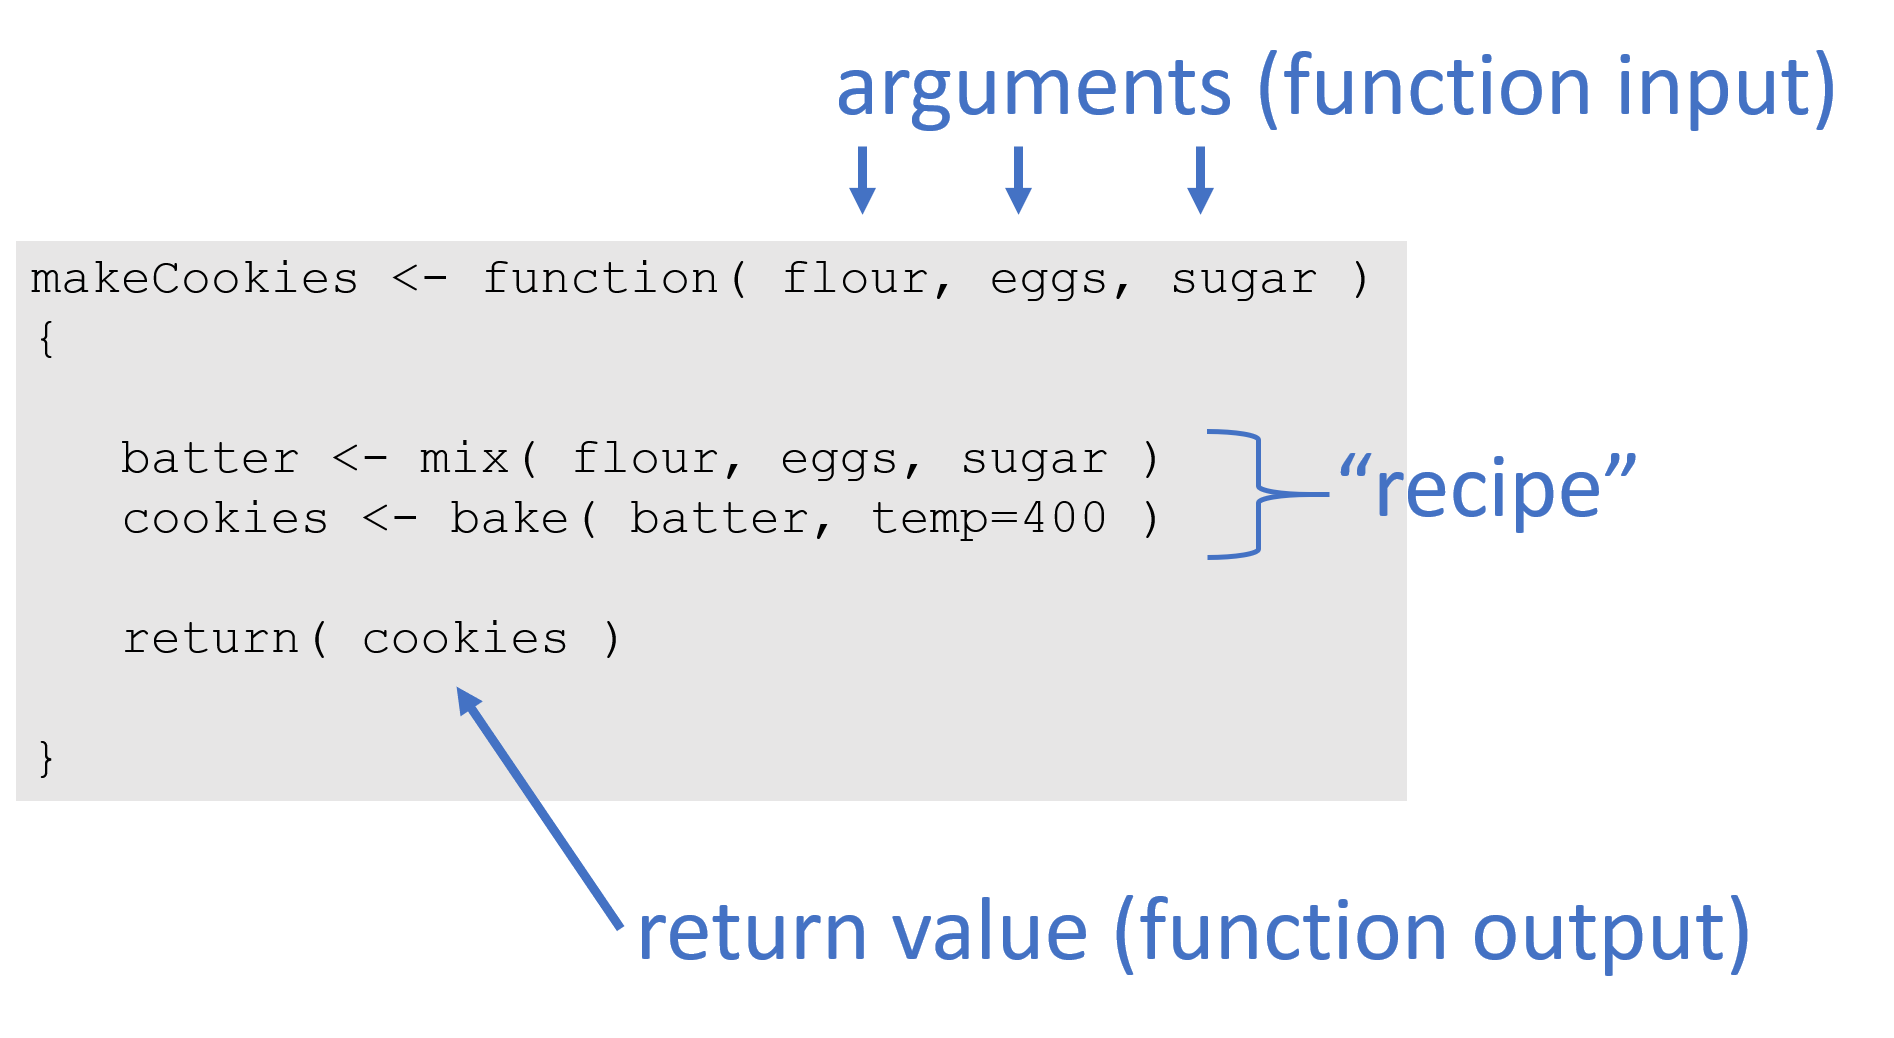
\includegraphics[width=0.7\linewidth]{figures/function} 

}

\caption{Anatomy of a function}\label{fig:unnamed-chunk-27}
\end{figure}

\begin{figure}

{\centering 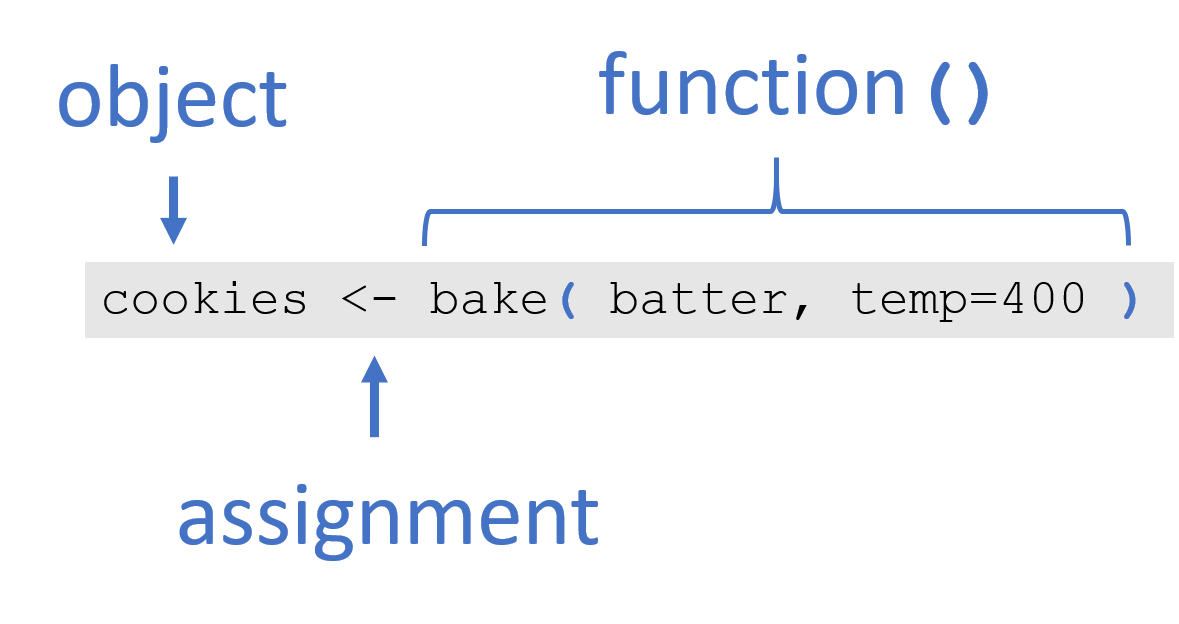
\includegraphics[width=0.7\linewidth]{figures/assignment} 

}

\caption{Assignment of output values}\label{fig:unnamed-chunk-28}
\end{figure}

After reading this chapter you should be able to define the following:

\begin{itemize}
\tightlist
\item
  function
\item
  argument
\item
  object
\item
  assignment
\end{itemize}

\hypertarget{computer-programs-as-recipes}{%
\section{Computer Programs as
Recipes}\label{computer-programs-as-recipes}}

Computer programs are powerful because they allow us to codify recipes
for complex tasks, save them, share them, and build upon them.

In the simplest form, a computer program is like a recipe. We have
inputs, steps, and outputs.

Ingredients:

\begin{itemize}
\tightlist
\item
  1/3 cup butter\\
\item
  1/2 cup sugar\\
\item
  1/4 cup brown sugar\\
\item
  2 teaspoons vanilla extract\\
\item
  1 large egg\\
\item
  2 cups all-purpose flour\\
\item
  1/2 teaspoon baking soda\\
\item
  1/2 teaspoon kosher salt\\
\item
  1 cup chocolate chips
\end{itemize}

Instructions:

\begin{enumerate}
\def\labelenumi{\arabic{enumi}.}
\tightlist
\item
  Preheat the oven to 375 degrees F.
\item
  In a large bowl, mix butter with the sugars until well-combined.
\item
  Stir in vanilla and egg until incorporated.
\item
  Addflour, baking soda, and salt.\\
\item
  Stir in chocolate chips.
\item
  Bake for 10 minutes.
\end{enumerate}

In R, the recipe would look something like this:

\begin{verbatim}
function( butter=0.33, sugar=0.5, eggs=1, flour=2, temp=375 )
{
   dry.goods <- combine( flour, sugar )
   batter <- mix( dry.goods, butter, eggs )
   cookies <- bake( batter, temp, time=10 )
   return( cookies )
}
\end{verbatim}

Note that this function to make cookies relies on other functions for
each step, combine(), mix(), and bake(). Each of these functions would
have to be defined as well, or more likely someone else in the open
source community has already written a package called ``baking'' that
contains simple functions for cooking so that you can use them for more
complicated recipes.

You will find that R allows you to conduct powerful analysis primarily
because you can build on top of and extend a lot of existing
functionality.

\hypertarget{example-function}{%
\section{Example Function}\label{example-function}}

As you get started in R you will be working with existing functions, not
writing your own. It is, however, constructive to see how one is
created. This example demonstrates the use of a mortgage calculator that
will take a loan size, term, and interest rate and return a monthly
payment.

\begin{Shaded}
\begin{Highlighting}[]
\NormalTok{   calcMortgage <-}\StringTok{ }\ControlFlowTok{function}\NormalTok{( principal, years, APR )}
\NormalTok{   \{}

\NormalTok{      months <-}\StringTok{ }\NormalTok{years }\OperatorTok{*}\StringTok{ }\DecValTok{12}
\NormalTok{      int.rate <-}\StringTok{ }\NormalTok{APR }\OperatorTok{/}\StringTok{ }\DecValTok{12}
      
      \CommentTok{# amortization formula}
\NormalTok{      monthly.payment <-}\StringTok{ }\NormalTok{( principal }\OperatorTok{*}\StringTok{ }\NormalTok{int.rate ) }\OperatorTok{/}\StringTok{ }
\StringTok{                         }\NormalTok{(}\DecValTok{1} \OperatorTok{-}\StringTok{ }\NormalTok{(}\DecValTok{1} \OperatorTok{+}\StringTok{ }\NormalTok{int.rate)}\OperatorTok{^}\NormalTok{(}\OperatorTok{-}\NormalTok{months) )}
      
\NormalTok{      monthly.payment <-}\StringTok{ }\KeywordTok{round}\NormalTok{( monthly.payment, }\DecValTok{2}\NormalTok{ )}
      
      \KeywordTok{return}\NormalTok{( monthly.payment )}
   
\NormalTok{   \}}
\end{Highlighting}
\end{Shaded}

Let's then see what the payments will be for a:

\begin{itemize}
\tightlist
\item
  \$100,000 loan
\item
  30-year mortgage
\item
  5\% annual interest rate
\end{itemize}

\begin{Shaded}
\begin{Highlighting}[]
\KeywordTok{calcMortgage}\NormalTok{( }\DataTypeTok{principal=}\DecValTok{100000}\NormalTok{, }\DataTypeTok{years=}\DecValTok{30}\NormalTok{, }\DataTypeTok{APR=}\FloatTok{0.05}\NormalTok{  )}
\CommentTok{### [1] 536.82}
\end{Highlighting}
\end{Shaded}

\hypertarget{default-argument-values}{%
\section{Default Argument Values}\label{default-argument-values}}

Note that the loan function needs all three of the input values in order
to calculate the loan size. If we were to omit one required value, we
would get an error.

\begin{Shaded}
\begin{Highlighting}[]
\KeywordTok{calcMortgage}\NormalTok{( }\DataTypeTok{principal=}\DecValTok{100000}\NormalTok{  )}
\CommentTok{# Error in calcMortgage(APR = 0.05, principal = 1e+05):  }
\CommentTok{#  argument "years" is missing, with no default }
\end{Highlighting}
\end{Shaded}

When creating functions, we might have a good idea of typical use cases.
If true, we can try to guess at reasonable user parameters. For example,
perhaps we are working at a bank where most of the customers take out
30-year mortgages, and interest rates have been stable at 5 percent. We
can set these as default values when we create the function.

\begin{Shaded}
\begin{Highlighting}[]
\NormalTok{   calcMortgage <-}\StringTok{ }\ControlFlowTok{function}\NormalTok{( principal, }\DataTypeTok{years=}\DecValTok{30}\NormalTok{, }\DataTypeTok{APR=}\FloatTok{0.05}\NormalTok{ )}
\NormalTok{   ...}
\end{Highlighting}
\end{Shaded}

We can now run the function while omitting arguments, as long as they
have defaults assigned.

\begin{Shaded}
\begin{Highlighting}[]
\KeywordTok{calcMortgage}\NormalTok{( }\DataTypeTok{principal=}\DecValTok{100000}\NormalTok{  )}
\CommentTok{### [1] 536.82}
\end{Highlighting}
\end{Shaded}

\hypertarget{assignment}{%
\section{Assignment}\label{assignment}}

When we call a function in R, the default behavior of the function is
typically to print the results on the screen:

\begin{Shaded}
\begin{Highlighting}[]
\KeywordTok{calcMortgage}\NormalTok{( }\DataTypeTok{principal=}\DecValTok{100000}\NormalTok{  )}
\CommentTok{### [1] 536.82}
\end{Highlighting}
\end{Shaded}

If we are creating a script, however, we often need to save the function
outputs at each step. We can do this by assigning output to a new
variable.

\begin{Shaded}
\begin{Highlighting}[]
\NormalTok{payments.}\FloatTok{15.}\NormalTok{year <-}\StringTok{ }\KeywordTok{calcMortgage}\NormalTok{( }\DataTypeTok{years=}\DecValTok{15}\NormalTok{, }\DataTypeTok{principal=}\DecValTok{100000}\NormalTok{  )}
\NormalTok{payments.}\FloatTok{30.}\NormalTok{year <-}\StringTok{ }\KeywordTok{calcMortgage}\NormalTok{( }\DataTypeTok{years=}\DecValTok{30}\NormalTok{, }\DataTypeTok{principal=}\DecValTok{100000}\NormalTok{  )}
\end{Highlighting}
\end{Shaded}

These values are then stored, and can be used later or printed by typing
the object name:

\begin{Shaded}
\begin{Highlighting}[]
\NormalTok{payments.}\FloatTok{15.}\NormalTok{year}
\CommentTok{### [1] 790.79}
\NormalTok{payments.}\FloatTok{30.}\NormalTok{year}
\CommentTok{### [1] 536.82}
\end{Highlighting}
\end{Shaded}

Note that variable names can include periods or underscores. They can
also include numbers, but they cannot start with a number. Like
everything in R, they will be case sensitive.

\hypertarget{data-structures}{%
\chapter{Data Structures}\label{data-structures}}

\hypertarget{key-concepts-1}{%
\section{Key Concepts}\label{key-concepts-1}}

\begin{figure}

{\centering 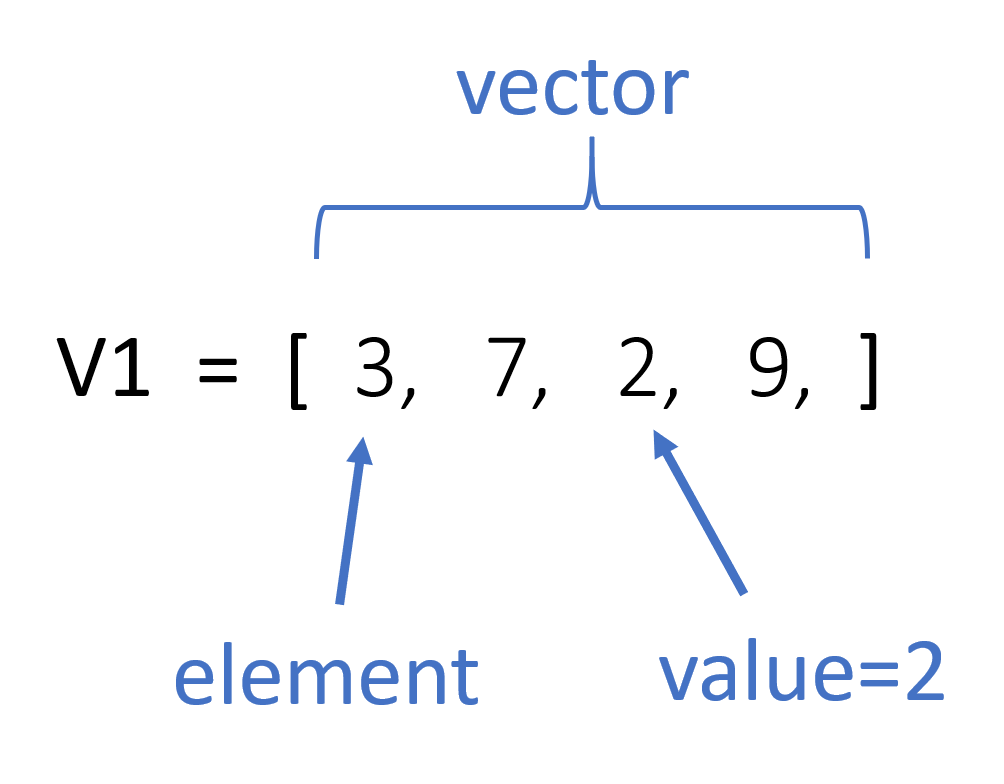
\includegraphics[width=0.7\linewidth]{figures/vectors} 

}

\caption{Components of a Vector}\label{fig:unnamed-chunk-40}
\end{figure}

\begin{figure}

{\centering 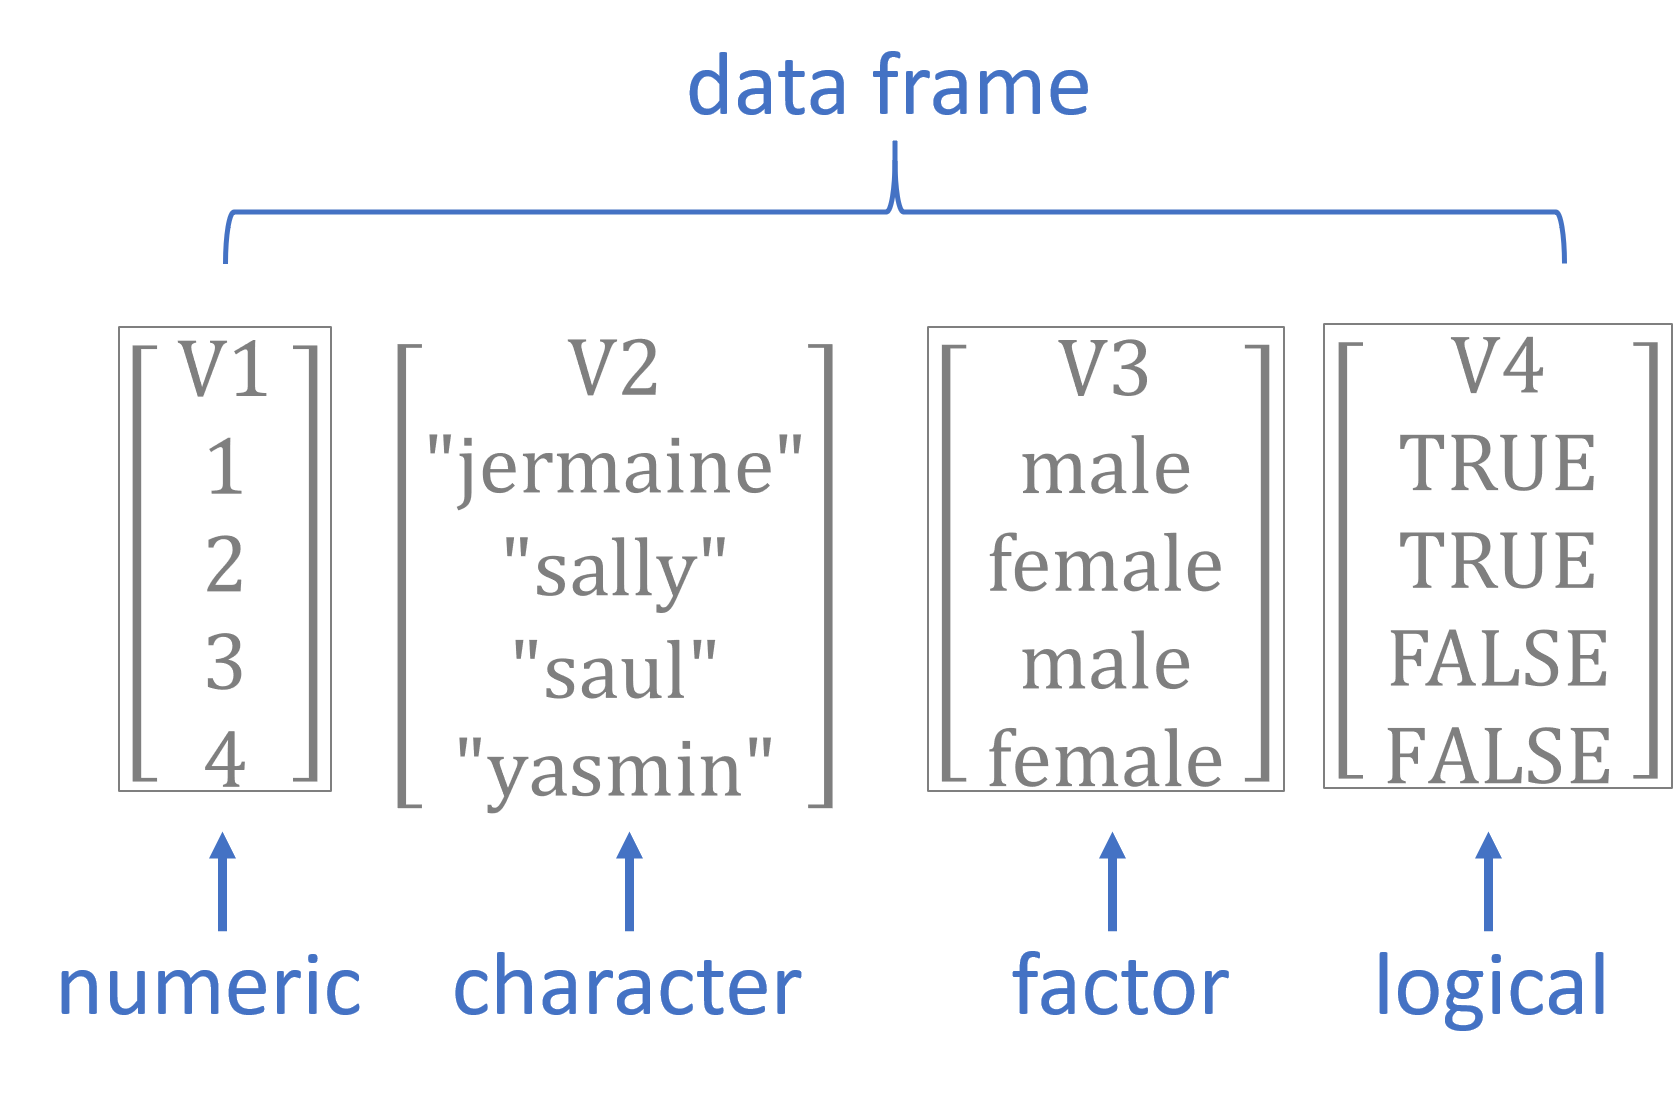
\includegraphics[width=0.7\linewidth]{figures/data_types} 

}

\caption{Basic data types in R}\label{fig:unnamed-chunk-41}
\end{figure}

\hypertarget{vectors}{%
\section{Vectors}\label{vectors}}

Vectors are the building blocks of data programming in R, so they are
extremely important concepts.

Very loosely speaking a vector is a set of numbers, words, or other
values:

\begin{itemize}
\tightlist
\item
  {[} 1, 2, 3{]}
\item
  {[} apple, orange, pear {]}
\item
  {[} TRUE, FALSE, FALSE {]}
\end{itemize}

In social sciences, a vector usually represents a variable in a dataset.

There are four primary vector types (``classes'') in R:

\begin{longtable}[]{@{}ll@{}}
\toprule
\begin{minipage}[b]{0.45\columnwidth}\raggedright
Class\strut
\end{minipage} & \begin{minipage}[b]{0.49\columnwidth}\raggedright
Description\strut
\end{minipage}\tabularnewline
\midrule
\endhead
\begin{minipage}[t]{0.45\columnwidth}\raggedright
numeric\strut
\end{minipage} & \begin{minipage}[t]{0.49\columnwidth}\raggedright
Typical variable of only numbers\strut
\end{minipage}\tabularnewline
\begin{minipage}[t]{0.45\columnwidth}\raggedright
character\strut
\end{minipage} & \begin{minipage}[t]{0.49\columnwidth}\raggedright
A vector of letters or words, always enclosed with quotes\strut
\end{minipage}\tabularnewline
\begin{minipage}[t]{0.45\columnwidth}\raggedright
factor\strut
\end{minipage} & \begin{minipage}[t]{0.49\columnwidth}\raggedright
Categories which represent groups, like treatment and control\strut
\end{minipage}\tabularnewline
\begin{minipage}[t]{0.45\columnwidth}\raggedright
logical\strut
\end{minipage} & \begin{minipage}[t]{0.49\columnwidth}\raggedright
A vector of TRUE and FALSE to designate which observations fit a
criteria\strut
\end{minipage}\tabularnewline
\bottomrule
\end{longtable}

Each vector or dataset has a ``class'' that tells R the data type.

These different vectors can be combined into three different types of
datasets (data frames, matrices, and lists), which will be discussed
below.

\begin{Shaded}
\begin{Highlighting}[]

\NormalTok{x1 <-}\StringTok{ }\KeywordTok{c}\NormalTok{(}\DecValTok{167}\NormalTok{,}\DecValTok{185}\NormalTok{,}\DecValTok{119}\NormalTok{,}\DecValTok{142}\NormalTok{)}

\NormalTok{x2 <-}\StringTok{ }\KeywordTok{c}\NormalTok{(}\StringTok{"adam"}\NormalTok{,}\StringTok{"jamal"}\NormalTok{,}\StringTok{"linda"}\NormalTok{,}\StringTok{"sriti"}\NormalTok{)}

\NormalTok{x3 <-}\StringTok{ }\KeywordTok{factor}\NormalTok{( }\KeywordTok{c}\NormalTok{(}\StringTok{"male"}\NormalTok{,}\StringTok{"male"}\NormalTok{,}\StringTok{"female"}\NormalTok{,}\StringTok{"female"}\NormalTok{) )}

\NormalTok{x4 <-}\StringTok{ }\KeywordTok{c}\NormalTok{( }\StringTok{"treatment"}\NormalTok{,}\StringTok{"control"}\NormalTok{,}\StringTok{"treatment"}\NormalTok{,}\StringTok{"control"}\NormalTok{ )}

\NormalTok{x5 <-}\StringTok{ }\NormalTok{x4 }\OperatorTok{==}\StringTok{ "treatment"}

\NormalTok{dat <-}\StringTok{ }\KeywordTok{data.frame}\NormalTok{( }\DataTypeTok{name=}\NormalTok{x2, }\DataTypeTok{sex=}\NormalTok{x3, }\DataTypeTok{treat=}\NormalTok{x4, }\DataTypeTok{is.treat=}\NormalTok{x5, }\DataTypeTok{strength=}\NormalTok{x1 )}
\end{Highlighting}
\end{Shaded}

\begin{longtable}[]{@{}ccccc@{}}
\toprule
\begin{minipage}[b]{0.10\columnwidth}\centering
name\strut
\end{minipage} & \begin{minipage}[b]{0.11\columnwidth}\centering
sex\strut
\end{minipage} & \begin{minipage}[b]{0.14\columnwidth}\centering
treat\strut
\end{minipage} & \begin{minipage}[b]{0.13\columnwidth}\centering
is.treat\strut
\end{minipage} & \begin{minipage}[b]{0.13\columnwidth}\centering
strength\strut
\end{minipage}\tabularnewline
\midrule
\endhead
\begin{minipage}[t]{0.10\columnwidth}\centering
adam\strut
\end{minipage} & \begin{minipage}[t]{0.11\columnwidth}\centering
male\strut
\end{minipage} & \begin{minipage}[t]{0.14\columnwidth}\centering
treatment\strut
\end{minipage} & \begin{minipage}[t]{0.13\columnwidth}\centering
TRUE\strut
\end{minipage} & \begin{minipage}[t]{0.13\columnwidth}\centering
167\strut
\end{minipage}\tabularnewline
\begin{minipage}[t]{0.10\columnwidth}\centering
jamal\strut
\end{minipage} & \begin{minipage}[t]{0.11\columnwidth}\centering
male\strut
\end{minipage} & \begin{minipage}[t]{0.14\columnwidth}\centering
control\strut
\end{minipage} & \begin{minipage}[t]{0.13\columnwidth}\centering
FALSE\strut
\end{minipage} & \begin{minipage}[t]{0.13\columnwidth}\centering
185\strut
\end{minipage}\tabularnewline
\begin{minipage}[t]{0.10\columnwidth}\centering
linda\strut
\end{minipage} & \begin{minipage}[t]{0.11\columnwidth}\centering
female\strut
\end{minipage} & \begin{minipage}[t]{0.14\columnwidth}\centering
treatment\strut
\end{minipage} & \begin{minipage}[t]{0.13\columnwidth}\centering
TRUE\strut
\end{minipage} & \begin{minipage}[t]{0.13\columnwidth}\centering
119\strut
\end{minipage}\tabularnewline
\begin{minipage}[t]{0.10\columnwidth}\centering
sriti\strut
\end{minipage} & \begin{minipage}[t]{0.11\columnwidth}\centering
female\strut
\end{minipage} & \begin{minipage}[t]{0.14\columnwidth}\centering
control\strut
\end{minipage} & \begin{minipage}[t]{0.13\columnwidth}\centering
FALSE\strut
\end{minipage} & \begin{minipage}[t]{0.13\columnwidth}\centering
142\strut
\end{minipage}\tabularnewline
\bottomrule
\end{longtable}

R keeps track of the data type of each object, which can be ascertained
using the \textbf{class()} function.

\begin{Shaded}
\begin{Highlighting}[]
\KeywordTok{class}\NormalTok{( x )}
\end{Highlighting}
\end{Shaded}

\begin{verbatim}
### $name
### [1] "character"
### 
### $sex
### [1] "factor"
### 
### $treat
### [1] "character"
### 
### $is.treat
### [1] "logical"
### 
### $strength
### [1] "numeric"
\end{verbatim}

\begin{Shaded}
\begin{Highlighting}[]
\KeywordTok{class}\NormalTok{( dat )}
\CommentTok{### [1] "data.frame"}
\end{Highlighting}
\end{Shaded}

\hypertarget{common-vectors-functions}{%
\section{Common Vectors Functions}\label{common-vectors-functions}}

You will spend a lot of time creating data vectors, transforming
variables, generating subsets, cleaning data, and adding new
observations. These are all accomplished through \textbf{functions()}
that act on vectors.

We often need to know how many elements belong to a vector, which we
find with the \textbf{length()} function.

\begin{Shaded}
\begin{Highlighting}[]
\NormalTok{x1}
\CommentTok{### [1] 167 185 119 142}

\KeywordTok{length}\NormalTok{( x1 )}
\CommentTok{### [1] 4}
\end{Highlighting}
\end{Shaded}

\hypertarget{the-combine-function}{%
\section{The Combine Function}\label{the-combine-function}}

We often need to combine several elements into a single vector, or
combine two vectors to form one. This is done using the \textbf{c()}
function.

\begin{Shaded}
\begin{Highlighting}[]

\KeywordTok{c}\NormalTok{(}\DecValTok{1}\NormalTok{,}\DecValTok{2}\NormalTok{,}\DecValTok{3}\NormalTok{)        }\CommentTok{# create a numeric vector}
\CommentTok{### [1] 1 2 3}

\KeywordTok{c}\NormalTok{(}\StringTok{"a"}\NormalTok{,}\StringTok{"b"}\NormalTok{,}\StringTok{"c"}\NormalTok{)  }\CommentTok{# create a character vector}
\CommentTok{### [1] "a" "b" "c"}
\end{Highlighting}
\end{Shaded}

Combining two vectors:

\begin{Shaded}
\begin{Highlighting}[]

\NormalTok{x <-}\StringTok{ }\DecValTok{1}\OperatorTok{:}\DecValTok{5}

\NormalTok{y <-}\StringTok{ }\DecValTok{10}\OperatorTok{:}\DecValTok{15}

\NormalTok{z <-}\StringTok{ }\KeywordTok{c}\NormalTok{(x,y)}

\NormalTok{z}
\CommentTok{###  [1]  1  2  3  4  5 10 11 12 13 14 15}
\end{Highlighting}
\end{Shaded}

Combining two vectors of different data types:

\begin{Shaded}
\begin{Highlighting}[]
\NormalTok{x <-}\StringTok{ }\KeywordTok{c}\NormalTok{(}\DecValTok{1}\NormalTok{,}\DecValTok{2}\NormalTok{,}\DecValTok{3}\NormalTok{)}

\NormalTok{y <-}\StringTok{ }\KeywordTok{c}\NormalTok{(}\StringTok{"a"}\NormalTok{,}\StringTok{"b"}\NormalTok{,}\StringTok{"c"}\NormalTok{)}

\NormalTok{z <-}\StringTok{ }\KeywordTok{c}\NormalTok{(x,y)}

\NormalTok{z}
\CommentTok{### [1] "1" "2" "3" "a" "b" "c"}
\end{Highlighting}
\end{Shaded}

\hypertarget{casting}{%
\section{Casting}\label{casting}}

You can easily move from one data type to another by \textbf{casting} a
specific type as another type:

\begin{Shaded}
\begin{Highlighting}[]

\NormalTok{x <-}\StringTok{ }\DecValTok{1}\OperatorTok{:}\DecValTok{5}

\NormalTok{x}
\CommentTok{### [1] 1 2 3 4 5}

\KeywordTok{as.character}\NormalTok{(x)}
\CommentTok{### [1] "1" "2" "3" "4" "5"}

\NormalTok{y <-}\StringTok{ }\KeywordTok{c}\NormalTok{(}\OtherTok{TRUE}\NormalTok{, }\OtherTok{FALSE}\NormalTok{, }\OtherTok{TRUE}\NormalTok{, }\OtherTok{TRUE}\NormalTok{, }\OtherTok{FALSE}\NormalTok{)}

\NormalTok{y}
\CommentTok{### [1]  TRUE FALSE  TRUE  TRUE FALSE}

\KeywordTok{as.numeric}\NormalTok{( y )}
\CommentTok{### [1] 1 0 1 1 0}

\KeywordTok{as.character}\NormalTok{( y )}
\CommentTok{### [1] "TRUE"  "FALSE" "TRUE"  "TRUE"  "FALSE"}
\end{Highlighting}
\end{Shaded}

But in some cases it might not make sense to cast one variable type as
another.

\begin{Shaded}
\begin{Highlighting}[]

\NormalTok{z <-}\StringTok{ }\KeywordTok{c}\NormalTok{(}\StringTok{"a"}\NormalTok{, }\StringTok{"b"}\NormalTok{, }\StringTok{"c"}\NormalTok{)}

\NormalTok{z}
\CommentTok{### [1] "a" "b" "c"}

\KeywordTok{as.numeric}\NormalTok{( z )}
\CommentTok{### [1] NA NA NA}
\end{Highlighting}
\end{Shaded}

Casting will often be induced automatically when you try to combine
different types of data. For example, when you add a character element
to a numeric vector, the whole vector will be cast as a character
vector.

\begin{Shaded}
\begin{Highlighting}[]

\NormalTok{x1 <-}\StringTok{ }\DecValTok{1}\OperatorTok{:}\DecValTok{5}
\NormalTok{x1}
\CommentTok{### [1] 1 2 3 4 5}

\NormalTok{x1 <-}\StringTok{ }\KeywordTok{c}\NormalTok{( x1, }\StringTok{"a"}\NormalTok{ ) }\CommentTok{# a vector can only have one data type}

\NormalTok{x1 }\CommentTok{# all numbers silently recast as characters}
\CommentTok{### [1] "1" "2" "3" "4" "5" "a"}
\end{Highlighting}
\end{Shaded}

If you consider the example above, when a numeric and character vector
are combined all elements are re-cast as strings because numbers can be
represented as characters but not vice-versa. R tries to select a
reasonable default type, but sometimes casting will create some strange
and unexpected behaviors. Consider some of these examples. What do you
think each will produce?

\begin{Shaded}
\begin{Highlighting}[]

\NormalTok{x1 <-}\StringTok{ }\KeywordTok{c}\NormalTok{(}\DecValTok{1}\NormalTok{,}\DecValTok{2}\NormalTok{,}\DecValTok{3}\NormalTok{)                    }\CommentTok{# numeric}
\NormalTok{x2 <-}\StringTok{ }\KeywordTok{c}\NormalTok{(}\StringTok{"a"}\NormalTok{,}\StringTok{"b"}\NormalTok{,}\StringTok{"c"}\NormalTok{)              }\CommentTok{# character}
\NormalTok{x3 <-}\StringTok{ }\KeywordTok{c}\NormalTok{(}\OtherTok{TRUE}\NormalTok{,}\OtherTok{FALSE}\NormalTok{,}\OtherTok{TRUE}\NormalTok{)          }\CommentTok{# logical}
\NormalTok{x4 <-}\StringTok{ }\KeywordTok{factor}\NormalTok{( }\KeywordTok{c}\NormalTok{(}\StringTok{"a"}\NormalTok{,}\StringTok{"b"}\NormalTok{,}\StringTok{"c"}\NormalTok{) )    }\CommentTok{# factor}

\NormalTok{case1 <-}\StringTok{ }\KeywordTok{c}\NormalTok{( x1, x3 )}

\NormalTok{case2 <-}\StringTok{ }\KeywordTok{c}\NormalTok{( x2, x3 )}

\NormalTok{case3 <-}\StringTok{ }\KeywordTok{c}\NormalTok{( x1, x4 )}

\NormalTok{case4 <-}\StringTok{ }\KeywordTok{c}\NormalTok{( x2, x4 )}
\end{Highlighting}
\end{Shaded}

The answers to \emph{case1} and \emph{case2} are somewhat intuitive.

\begin{Shaded}
\begin{Highlighting}[]
\NormalTok{case1  }\CommentTok{# combine a numeric and logical vector}
\CommentTok{### [1] 1 2 3 1 0 1}

\NormalTok{case2  }\CommentTok{# combine a character and logical vector}
\CommentTok{### [1] "a"     "b"     "c"     "TRUE"  "FALSE" "TRUE"}
\end{Highlighting}
\end{Shaded}

Recall that TRUE and FALSE are often represented as 1 and 0 in datasets,
so they can be recast as numeric elements. The numbers 2 and 3 have no
meaning in a logical vector, so we can't cast a numeric vector as a
logical vector.

\emph{case3} and \emph{case4} are a little more nuanced. See the section
on factors below to make sense of them.

\begin{Shaded}
\begin{Highlighting}[]
\NormalTok{case3  }\CommentTok{# combine a numeric and factor vector}
\CommentTok{### [1] 1 2 3 1 2 3}

\NormalTok{case4  }\CommentTok{# combine a character and factor vector}
\CommentTok{### [1] "a" "b" "c" "1" "2" "3"}
\end{Highlighting}
\end{Shaded}

TIP: When you read data in from outside sources, the input functions
often will cast character or numeric vectors as factors if they contain
a low number of elements. See the section on factors below for special
instructions on moving from factors to numeric vectors.

\hypertarget{numeric-vectors}{%
\section{Numeric Vectors}\label{numeric-vectors}}

There are some specific things to note about each vector type.

Math operators will only work on numeric vectors.

\begin{Shaded}
\begin{Highlighting}[]

\KeywordTok{summary}\NormalTok{( x1 )}
\CommentTok{###    Min. 1st Qu.  Median    Mean 3rd Qu.    Max. }
\CommentTok{###     1.0     1.5     2.0     2.0     2.5     3.0}
\end{Highlighting}
\end{Shaded}

Note that if we try to run this mathematicl function we get an error:

\begin{Shaded}
\begin{Highlighting}[]

\KeywordTok{sum}\NormalTok{( x2 ) }\CommentTok{# Error in sum(x2) : invalid 'type' (character) of argument}
\end{Highlighting}
\end{Shaded}

Many functions in R are sensitive to the data type of vectors.
Mathematical functions, for example, do not make sense when applied to
text (character vectors). In many cases R will give an error. In some
cases R will silently re-cast the variable, then perform the operation.
Be watchful for when silent re-casting occurs because it might have
unwanted side effects, such as deleting data or re-coding group levels
in the wrong way.

\hypertarget{integers-are-simple-numeric-vectors}{%
\subsection{Integers Are Simple Numeric
Vectors}\label{integers-are-simple-numeric-vectors}}

The integer vector is a special type of numeric vector. It is used to
save memory since integers require less space than numbers that contain
decimals points (you need to allocate space for the numbers to the left
and the numbers to the right of the decimal). Google ``computer memory
allocation'' if you are interested in the specifics.

If you are doing advanced programming you will be more sensitive to
memory allocation and the speed of your code, but in the intro class we
will not differentiate between the two types of number vectors. In
\emph{most} cases they result in the same results, unless you are doing
advanced numerical analysis where rounding errors matter.

\begin{Shaded}
\begin{Highlighting}[]

\NormalTok{n <-}\StringTok{ }\DecValTok{1}\OperatorTok{:}\DecValTok{5}

\NormalTok{n}
\CommentTok{### [1] 1 2 3 4 5}

\KeywordTok{class}\NormalTok{( n )}
\CommentTok{### [1] "integer"}

\NormalTok{n[ }\DecValTok{2}\NormalTok{ ] <-}\StringTok{ }\FloatTok{2.01}

\NormalTok{n  }\CommentTok{# all elements converted to decimals}
\CommentTok{### [1] 1.00 2.01 3.00 4.00 5.00}

\KeywordTok{class}\NormalTok{( n )}
\CommentTok{### [1] "numeric"}
\end{Highlighting}
\end{Shaded}

\hypertarget{character-vectors}{%
\section{Character Vectors}\label{character-vectors}}

The most important rule to remember with this data type: when creating
character vectors, all text must be enclosed by quotation marks.

This one works:

\begin{Shaded}
\begin{Highlighting}[]

\KeywordTok{c}\NormalTok{( }\StringTok{"a"}\NormalTok{, }\StringTok{"b"}\NormalTok{, }\StringTok{"c"}\NormalTok{ )   }\CommentTok{# this works}
\CommentTok{### [1] "a" "b" "c"}
\end{Highlighting}
\end{Shaded}

This one will not:

\begin{Shaded}
\begin{Highlighting}[]
\KeywordTok{c}\NormalTok{( a, b, c )  }
\CommentTok{# Error: object 'a' not found}
\end{Highlighting}
\end{Shaded}

When you type characters surrounded by quotes then R knows you are
creating new text (``strings'' in programming speak). When you type
characters that are not surrounded by quotes, R thinks that you are
looking for an object in the environment, like the variables we have
already created. It gets confused when it doesn't find the object that
you typed.

In generate, you will use quotes when you are creating character
vectors, and for arguments in functions. You do not use quotes when you
are referencing an active object. An active object is typically a
dataset or vector that you have imported or created. You can print a
list of all active objects with the \texttt{ls()} function.

\hypertarget{quotes-in-arguments}{%
\subsection{Quotes in Arguments}\label{quotes-in-arguments}}

When you first start using R it can be confusing about when quotes are
needed around arguments. Take the following example of the color
argument (\texttt{col=}) in the \texttt{plot()} function.

\begin{Shaded}
\begin{Highlighting}[]
\NormalTok{strength <-}\StringTok{ }\KeywordTok{c}\NormalTok{(}\DecValTok{167}\NormalTok{,}\DecValTok{185}\NormalTok{,}\DecValTok{119}\NormalTok{,}\DecValTok{142}\NormalTok{)}
\NormalTok{name <-}\StringTok{ }\KeywordTok{c}\NormalTok{(}\StringTok{"adam"}\NormalTok{,}\StringTok{"jamal"}\NormalTok{,}\StringTok{"linda"}\NormalTok{,}\StringTok{"sriti"}\NormalTok{)}
\NormalTok{group <-}\StringTok{ }\KeywordTok{factor}\NormalTok{( }\KeywordTok{c}\NormalTok{( }\StringTok{"treatment"}\NormalTok{,}\StringTok{"control"}\NormalTok{,}\StringTok{"treatment"}\NormalTok{,}\StringTok{"control"}\NormalTok{ ) )}

\KeywordTok{plot}\NormalTok{( strength, }\DataTypeTok{col=}\StringTok{"blue"}\NormalTok{, ... )}

\KeywordTok{plot}\NormalTok{( strength, }\DataTypeTok{col=}\NormalTok{group,  ... )}
\end{Highlighting}
\end{Shaded}

\begin{center}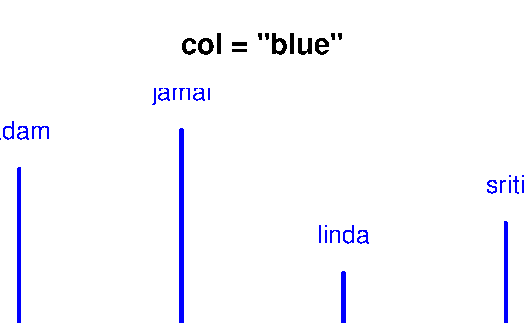
\includegraphics[width=0.7\linewidth]{DS4PS-I_files/figure-latex/unnamed-chunk-63-1} 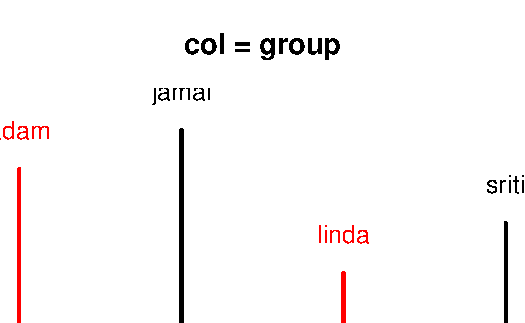
\includegraphics[width=0.7\linewidth]{DS4PS-I_files/figure-latex/unnamed-chunk-63-2} \end{center}

In the first example we are using a text string as an argument to
specify a color (\texttt{col="blue"}), so it must be enclosed by quotes
because it is text.

In the second example R selects the color based upon group membership
specified by the factor called `group' (treatment or control). Since the
argument is now referencing an object (\texttt{col=group}), we do not
use quotes.

The exception here is when your argument requires a number. Numbers are
not passed with quotes, or they would be cast as text.

\hypertarget{factors}{%
\section{Factors}\label{factors}}

When there are categorical variables within our data, or groups, then we
use a special vector to keep track of these groups. We could just use
numbers (1=female, 0=male) or characters (``male'',``female''), but
factors are useful for two reasons.

First, it saves memory. Text is very ``expensive'' in terms of memory
allocation and processing speed, so using simpler data structure makes R
faster.

Second, when a variable is set as a factor, R recognizes that it
represents a group and it can deploy object-oriented functionality. When
you use a factor in analysis, R knows that you want to split the
analysis up by groups.

\begin{Shaded}
\begin{Highlighting}[]
\NormalTok{height <-}\StringTok{ }\KeywordTok{c}\NormalTok{( }\DecValTok{70}\NormalTok{, }\DecValTok{68}\NormalTok{, }\DecValTok{62}\NormalTok{, }\DecValTok{64}\NormalTok{, }\DecValTok{72}\NormalTok{, }\DecValTok{69}\NormalTok{, }\DecValTok{58}\NormalTok{, }\DecValTok{63}\NormalTok{  )}

\NormalTok{strength <-}\StringTok{ }\KeywordTok{c}\NormalTok{(}\DecValTok{167}\NormalTok{,}\DecValTok{185}\NormalTok{,}\DecValTok{119}\NormalTok{,}\DecValTok{142}\NormalTok{,}\DecValTok{175}\NormalTok{,}\DecValTok{204}\NormalTok{,}\DecValTok{124}\NormalTok{,}\DecValTok{117}\NormalTok{)}

\NormalTok{sex <-}\StringTok{ }\KeywordTok{factor}\NormalTok{( }\KeywordTok{c}\NormalTok{(}\StringTok{"male"}\NormalTok{,}\StringTok{"male"}\NormalTok{,}\StringTok{"female"}\NormalTok{,}\StringTok{"female"}\NormalTok{,}\StringTok{"male"}\NormalTok{,}\StringTok{"male"}\NormalTok{,}\StringTok{"female"}\NormalTok{,}\StringTok{"female"}\NormalTok{ ) )}

\KeywordTok{plot}\NormalTok{( height, strength )   }\CommentTok{# simple scatter plot}

\KeywordTok{plot}\NormalTok{( sex, strength )      }\CommentTok{# box and whisker plot       }
\end{Highlighting}
\end{Shaded}

\begin{center}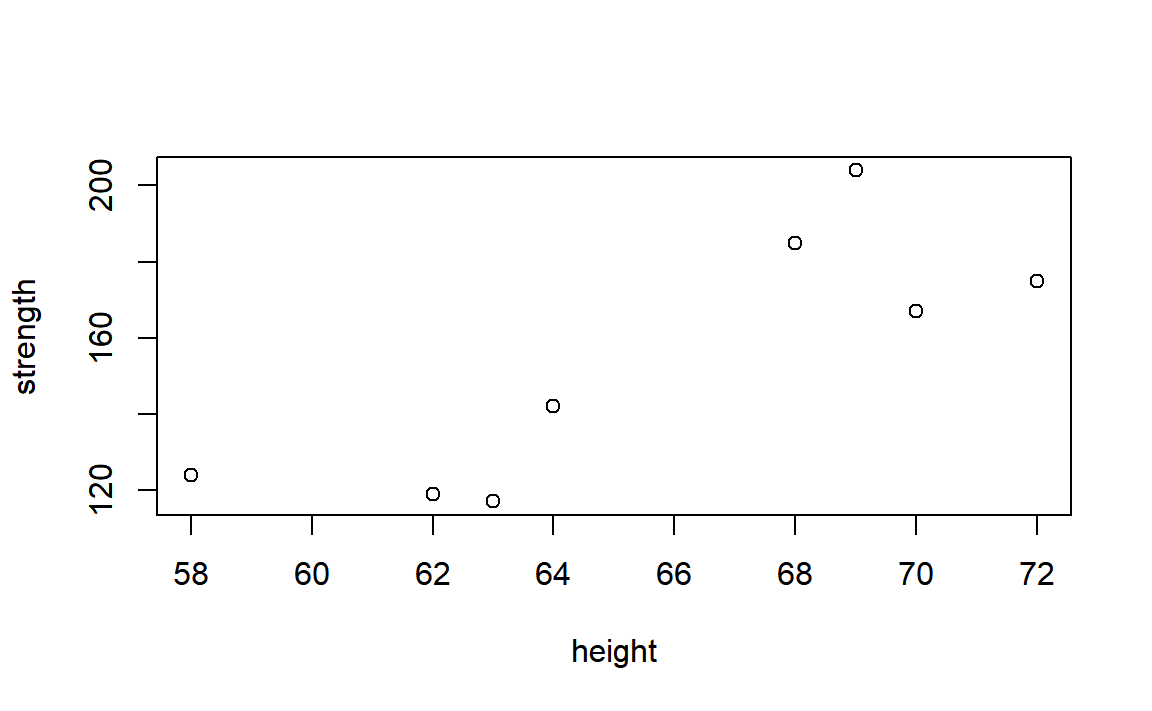
\includegraphics[width=0.7\linewidth]{DS4PS-I_files/figure-latex/unnamed-chunk-64-1} 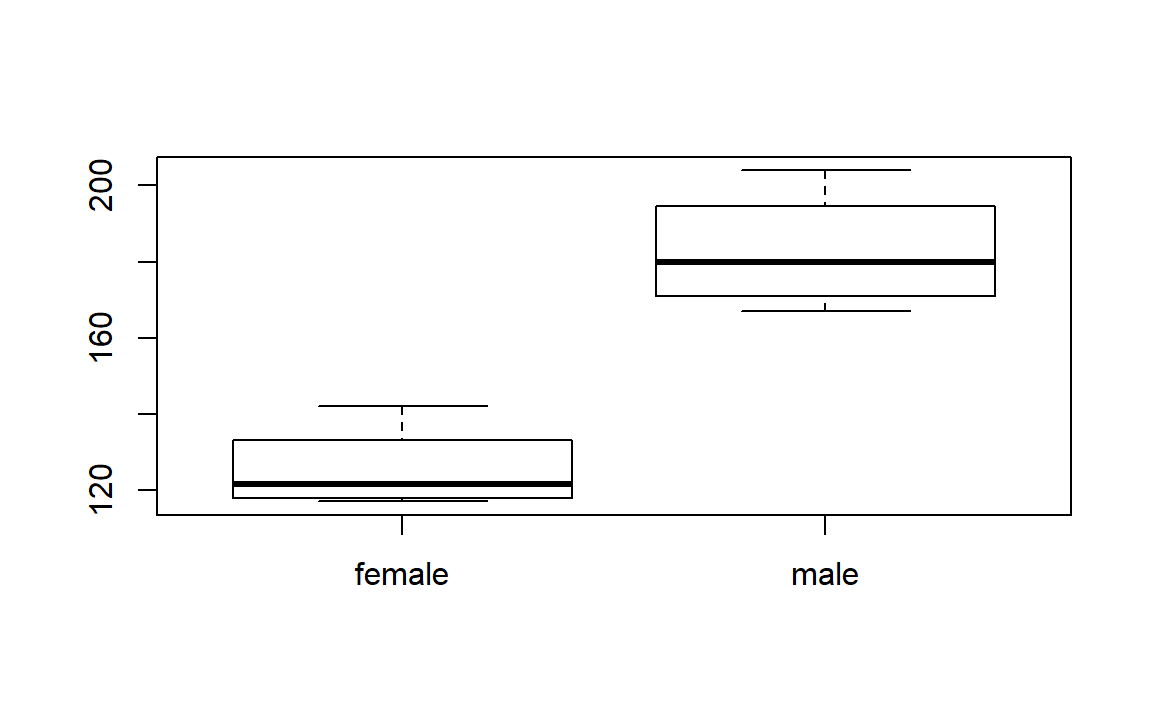
\includegraphics[width=0.7\linewidth]{DS4PS-I_files/figure-latex/unnamed-chunk-64-2} \end{center}

Factors are more memory efficient than character vectors because they
store the underlying data as a numeric vector instead of a categorical
(text) vector. Each group in the data is assigned a number, and when
printing items the program only has to remember which group corresponds
to which number:

\begin{Shaded}
\begin{Highlighting}[]
\NormalTok{sex}
\CommentTok{### [1] male   male   female female male   male   female female}
\CommentTok{### Levels: female male}

\KeywordTok{as.numeric}\NormalTok{( sex )}
\CommentTok{### [1] 2 2 1 1 2 2 1 1}

\CommentTok{#  male = 2}
\CommentTok{#  female = 1}
\end{Highlighting}
\end{Shaded}

If you print a factor, the computer just replaces each category
designation with its name (2 would be replaced with ``male'' in this
example). These replacements can be done in real time without clogging
the memory of your computer as they don't need to be saved.

In some instances a categorical variable might be represented by
numbers. For example, grades 9-12 for high school kids. The \textbf{very
important} rule to remember with factors is you can't move directly from
the factor to numeric using the \textbf{as.numeric()} casting function.
This will give you the underlying data structure, but will not give you
the category names. To get these, you need the \textbf{as.character}
casting function.

\begin{Shaded}
\begin{Highlighting}[]

\NormalTok{grades <-}\StringTok{ }\KeywordTok{sample}\NormalTok{( }\DataTypeTok{x=}\DecValTok{9}\OperatorTok{:}\DecValTok{12}\NormalTok{, }\DataTypeTok{size=}\DecValTok{10}\NormalTok{, }\DataTypeTok{replace=}\NormalTok{T )}

\NormalTok{grades}
\CommentTok{###  [1]  9 11 10 10 10  9 10 10 10  9}

\NormalTok{grades <-}\StringTok{ }\KeywordTok{as.factor}\NormalTok{( grades )}

\NormalTok{grades}
\CommentTok{###  [1] 9  11 10 10 10 9  10 10 10 9 }
\CommentTok{### Levels: 9 10 11}

\KeywordTok{as.numeric}\NormalTok{( grades )}
\CommentTok{###  [1] 1 3 2 2 2 1 2 2 2 1}

\KeywordTok{as.character}\NormalTok{( grades )}
\CommentTok{###  [1] "9"  "11" "10" "10" "10" "9"  "10" "10" "10" "9"}

\CommentTok{# to get back to the original numeric vector}

\KeywordTok{as.numeric}\NormalTok{( }\KeywordTok{as.character}\NormalTok{( grades ))}
\CommentTok{###  [1]  9 11 10 10 10  9 10 10 10  9}
\end{Highlighting}
\end{Shaded}

Note that when subsetting a factor, it will retain all of the original
levels, even when they are not in use.

In this example, there are 37 teams in the Lahman dataset (some of them
defunct) and 16 teams in the National League in 2002. But after applying
the year and league subsets you will still have 37 levels.

\begin{Shaded}
\begin{Highlighting}[]

\CommentTok{# there are only 16 teams in the NL in 2002}

\NormalTok{sals}\FloatTok{.2002}\NormalTok{ <-}\StringTok{ }\NormalTok{Salaries [Salaries}\OperatorTok{$}\NormalTok{yearID}\OperatorTok{==}\StringTok{"2002"}\NormalTok{, ]}
\NormalTok{nl.sals <-}\StringTok{ }\NormalTok{sals}\FloatTok{.2002}\NormalTok{ [ sals}\FloatTok{.2002}\OperatorTok{$}\NormalTok{lgID }\OperatorTok{==}\StringTok{ "NL"}\NormalTok{,]}
\KeywordTok{levels}\NormalTok{( nl.sals}\OperatorTok{$}\NormalTok{teamID )}
\CommentTok{###  [1] "ANA" "ARI" "ATL" "BAL" "BOS" "CAL" "CHA" "CHC" "CHN" "CHW" "CIN"}
\CommentTok{### [12] "CLE" "COL" "DET" "FLO" "HOU" "KCA" "KCR" "LAA" "LAD" "LAN" "MIA"}
\CommentTok{### [23] "MIL" "MIN" "ML4" "MON" "NYA" "NYM" "NYN" "NYY" "OAK" "PHI" "PIT"}
\CommentTok{### [34] "SDN" "SDP" "SEA" "SFG" "SFN" "SLN" "STL" "TBA" "TBR" "TEX" "TOR"}
\CommentTok{### [45] "WAS" "WSN"}
\end{Highlighting}
\end{Shaded}

After applying a subset, in order to remove the unused factor levels you
need to apply either droplevels(), or else recast your factor as a new
factor.

For example:

\begin{Shaded}
\begin{Highlighting}[]

\NormalTok{sals}\FloatTok{.2002}\NormalTok{ <-}\StringTok{ }\NormalTok{Salaries [Salaries}\OperatorTok{$}\NormalTok{yearID}\OperatorTok{==}\StringTok{"2002"}\NormalTok{, ]}

\NormalTok{nl.sals <-}\StringTok{ }\NormalTok{sals}\FloatTok{.2002}\NormalTok{ [ sals}\FloatTok{.2002}\OperatorTok{$}\NormalTok{lgID }\OperatorTok{==}\StringTok{ "NL"}\NormalTok{,]}
\KeywordTok{levels}\NormalTok{( nl.sals}\OperatorTok{$}\NormalTok{teamID )}
\CommentTok{###  [1] "ANA" "ARI" "ATL" "BAL" "BOS" "CAL" "CHA" "CHC" "CHN" "CHW" "CIN"}
\CommentTok{### [12] "CLE" "COL" "DET" "FLO" "HOU" "KCA" "KCR" "LAA" "LAD" "LAN" "MIA"}
\CommentTok{### [23] "MIL" "MIN" "ML4" "MON" "NYA" "NYM" "NYN" "NYY" "OAK" "PHI" "PIT"}
\CommentTok{### [34] "SDN" "SDP" "SEA" "SFG" "SFN" "SLN" "STL" "TBA" "TBR" "TEX" "TOR"}
\CommentTok{### [45] "WAS" "WSN"}

\CommentTok{# fix in one of two equivalent ways:}
\CommentTok{#}
\CommentTok{# nl.sals$teamID <- droplevels( nl.sals$teamID )}
\CommentTok{# nl.sals$teamID <- factor( nl.sals$teamID )}

\KeywordTok{levels}\NormalTok{( nl.sals}\OperatorTok{$}\NormalTok{teamID )}
\CommentTok{###  [1] "ANA" "ARI" "ATL" "BAL" "BOS" "CAL" "CHA" "CHC" "CHN" "CHW" "CIN"}
\CommentTok{### [12] "CLE" "COL" "DET" "FLO" "HOU" "KCA" "KCR" "LAA" "LAD" "LAN" "MIA"}
\CommentTok{### [23] "MIL" "MIN" "ML4" "MON" "NYA" "NYM" "NYN" "NYY" "OAK" "PHI" "PIT"}
\CommentTok{### [34] "SDN" "SDP" "SEA" "SFG" "SFN" "SLN" "STL" "TBA" "TBR" "TEX" "TOR"}
\CommentTok{### [45] "WAS" "WSN"}
\NormalTok{nl.sals}\OperatorTok{$}\NormalTok{teamID <-}\StringTok{ }\KeywordTok{droplevels}\NormalTok{( nl.sals}\OperatorTok{$}\NormalTok{teamID )}
\KeywordTok{levels}\NormalTok{( nl.sals}\OperatorTok{$}\NormalTok{teamID )}
\CommentTok{###  [1] "ARI" "ATL" "CHN" "CIN" "COL" "FLO" "HOU" "LAN" "MIL" "MON" "NYN"}
\CommentTok{### [12] "PHI" "PIT" "SDN" "SFN" "SLN"}
\end{Highlighting}
\end{Shaded}

TIP: When reading data from Excel spreadsheets (usually saved in the
comma separated value or CSV format), remember to include the following
argument to prevent the creation of factors, which can produce some
annoying behaviors.

\begin{Shaded}
\begin{Highlighting}[]

\NormalTok{dat <-}\StringTok{ }\KeywordTok{read.csv}\NormalTok{( }\StringTok{"filename.csv"}\NormalTok{, }\DataTypeTok{stringsAsFactors=}\NormalTok{F )}
\end{Highlighting}
\end{Shaded}

\hypertarget{generating-vectors}{%
\section{Generating Vectors}\label{generating-vectors}}

You will often need to generate vectors for data transformations or
simulations. Here are the most common functions that will be helpful.

\begin{Shaded}
\begin{Highlighting}[]

\CommentTok{# repeat a number, or series of numbers}

\KeywordTok{rep}\NormalTok{( }\DataTypeTok{x=}\DecValTok{9}\NormalTok{, }\DataTypeTok{times=}\DecValTok{5}\NormalTok{ )}
\CommentTok{### [1] 9 9 9 9 9}

\KeywordTok{rep}\NormalTok{( }\DataTypeTok{x=}\KeywordTok{c}\NormalTok{(}\DecValTok{5}\NormalTok{,}\DecValTok{7}\NormalTok{), }\DataTypeTok{times=}\DecValTok{5}\NormalTok{ )}
\CommentTok{###  [1] 5 7 5 7 5 7 5 7 5 7}

\KeywordTok{rep}\NormalTok{( }\DataTypeTok{x=}\KeywordTok{c}\NormalTok{(}\DecValTok{5}\NormalTok{,}\DecValTok{7}\NormalTok{), }\DataTypeTok{each=}\DecValTok{5}\NormalTok{ )}
\CommentTok{###  [1] 5 5 5 5 5 7 7 7 7 7}

\KeywordTok{rep}\NormalTok{( }\DataTypeTok{x=}\KeywordTok{c}\NormalTok{(}\StringTok{"treatment"}\NormalTok{,}\StringTok{"control"}\NormalTok{), }\DataTypeTok{each=}\DecValTok{5}\NormalTok{ )  }\CommentTok{# also works to create categories}
\CommentTok{###  [1] "treatment" "treatment" "treatment" "treatment" "treatment"}
\CommentTok{###  [6] "control"   "control"   "control"   "control"   "control"}


\CommentTok{# create a sequence of numbers}

\KeywordTok{seq}\NormalTok{( }\DataTypeTok{from=}\DecValTok{1}\NormalTok{, }\DataTypeTok{to=}\DecValTok{15}\NormalTok{, }\DataTypeTok{by=}\DecValTok{1}\NormalTok{ )}
\CommentTok{###  [1]  1  2  3  4  5  6  7  8  9 10 11 12 13 14 15}

\KeywordTok{seq}\NormalTok{( }\DataTypeTok{from=}\DecValTok{1}\NormalTok{, }\DataTypeTok{to=}\DecValTok{15}\NormalTok{, }\DataTypeTok{by=}\DecValTok{3}\NormalTok{ )}
\CommentTok{### [1]  1  4  7 10 13}

\DecValTok{1}\OperatorTok{:}\DecValTok{15}   \CommentTok{# shorthand if by=1}
\CommentTok{###  [1]  1  2  3  4  5  6  7  8  9 10 11 12 13 14 15}



\CommentTok{# create a random sample}

\NormalTok{hat <-}\StringTok{ }\KeywordTok{c}\NormalTok{(}\StringTok{"a"}\NormalTok{,}\StringTok{"b"}\NormalTok{,}\StringTok{"c"}\NormalTok{,}\StringTok{"b"}\NormalTok{,}\StringTok{"f"}\NormalTok{)}

\KeywordTok{sample}\NormalTok{( }\DataTypeTok{x=}\NormalTok{hat, }\DataTypeTok{size=}\DecValTok{3}\NormalTok{, }\DataTypeTok{replace=}\OtherTok{FALSE}\NormalTok{ )}
\CommentTok{### [1] "c" "b" "b"}
\KeywordTok{sample}\NormalTok{( }\DataTypeTok{x=}\NormalTok{hat, }\DataTypeTok{size=}\DecValTok{3}\NormalTok{, }\DataTypeTok{replace=}\OtherTok{FALSE}\NormalTok{ )}
\CommentTok{### [1] "f" "a" "b"}
\KeywordTok{sample}\NormalTok{( }\DataTypeTok{x=}\NormalTok{hat, }\DataTypeTok{size=}\DecValTok{3}\NormalTok{, }\DataTypeTok{replace=}\OtherTok{FALSE}\NormalTok{ )}
\CommentTok{### [1] "a" "f" "c"}

\CommentTok{# for multiple samples use replacement}

\KeywordTok{sample}\NormalTok{( }\DataTypeTok{x=}\NormalTok{hat, }\DataTypeTok{size=}\DecValTok{10}\NormalTok{, }\DataTypeTok{replace=}\OtherTok{TRUE}\NormalTok{ )}
\CommentTok{###  [1] "c" "a" "a" "b" "b" "a" "c" "b" "f" "f"}





\CommentTok{# create data that follows a normal curve}

\NormalTok{iq <-}\StringTok{ }\KeywordTok{rnorm}\NormalTok{( }\DataTypeTok{n=}\DecValTok{1000}\NormalTok{, }\DataTypeTok{mean=}\DecValTok{100}\NormalTok{, }\DataTypeTok{sd=}\DecValTok{15}\NormalTok{ )}

\KeywordTok{hist}\NormalTok{( iq, }\DataTypeTok{col=}\StringTok{"gray"}\NormalTok{ )}
\end{Highlighting}
\end{Shaded}

\begin{center}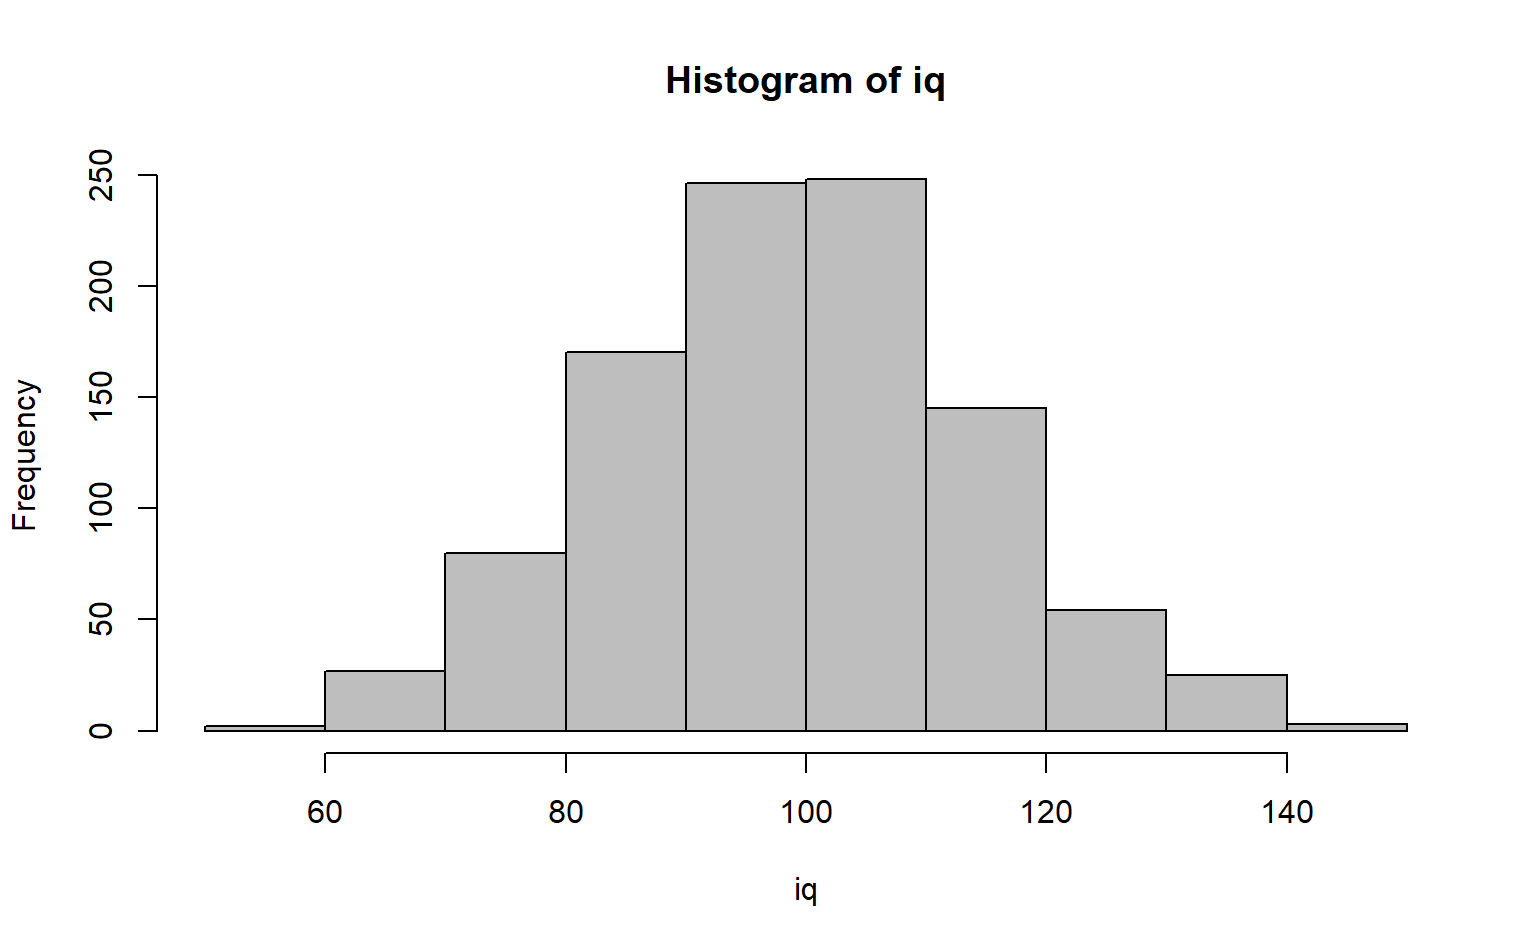
\includegraphics[width=0.7\linewidth]{DS4PS-I_files/figure-latex/unnamed-chunk-70-1} \end{center}

\hypertarget{variable-transformations}{%
\section{Variable Transformations}\label{variable-transformations}}

When we create a new variable from existing variables, it is called a
`transformation'. This is very common in data science. Crime is measures
by the number of assults \emph{per 100,000 people}, for example (crime /
pop). A batting average is the number of hits divided by the number of
at bats.

In R, mathematical operations are \emph{vectorized}, which means that
operations are performed on the entire vector all at once. This makes
transformations fast and easy.

\begin{Shaded}
\begin{Highlighting}[]

\NormalTok{x <-}\StringTok{ }\DecValTok{1}\OperatorTok{:}\DecValTok{10}

\NormalTok{x }\OperatorTok{+}\StringTok{ }\DecValTok{5}
\CommentTok{###  [1]  6  7  8  9 10 11 12 13 14 15}

\NormalTok{x }\OperatorTok{*}\StringTok{ }\DecValTok{5}
\CommentTok{###  [1]  5 10 15 20 25 30 35 40 45 50}
\end{Highlighting}
\end{Shaded}

R uses a convention called ``recycling'', which means that it will
re-use elements of a vector if necessary. In the example below the x
vector has 10 elements, but the y vector only has 5 elements. When we
run out of y, we just start over from the beginning. This is powerful in
some instances, but can be dangerous in others if you don't realize that
that it is happening.

\begin{Shaded}
\begin{Highlighting}[]

\NormalTok{x <-}\StringTok{ }\DecValTok{1}\OperatorTok{:}\DecValTok{10}

\NormalTok{y <-}\StringTok{ }\DecValTok{1}\OperatorTok{:}\DecValTok{5}

\NormalTok{x }\OperatorTok{+}\StringTok{ }\NormalTok{y}
\CommentTok{###  [1]  2  4  6  8 10  7  9 11 13 15}

\NormalTok{x }\OperatorTok{*}\StringTok{ }\NormalTok{y}
\CommentTok{###  [1]  1  4  9 16 25  6 14 24 36 50}

\CommentTok{# the colors are recycled}

\KeywordTok{plot}\NormalTok{( }\DecValTok{1}\OperatorTok{:}\DecValTok{5}\NormalTok{, }\DecValTok{1}\OperatorTok{:}\DecValTok{5}\NormalTok{, }\DataTypeTok{col=}\KeywordTok{c}\NormalTok{(}\StringTok{"red"}\NormalTok{,}\StringTok{"blue"}\NormalTok{), }\DataTypeTok{pch=}\DecValTok{19}\NormalTok{, }\DataTypeTok{cex=}\DecValTok{3}\NormalTok{ )}
\end{Highlighting}
\end{Shaded}

\begin{center}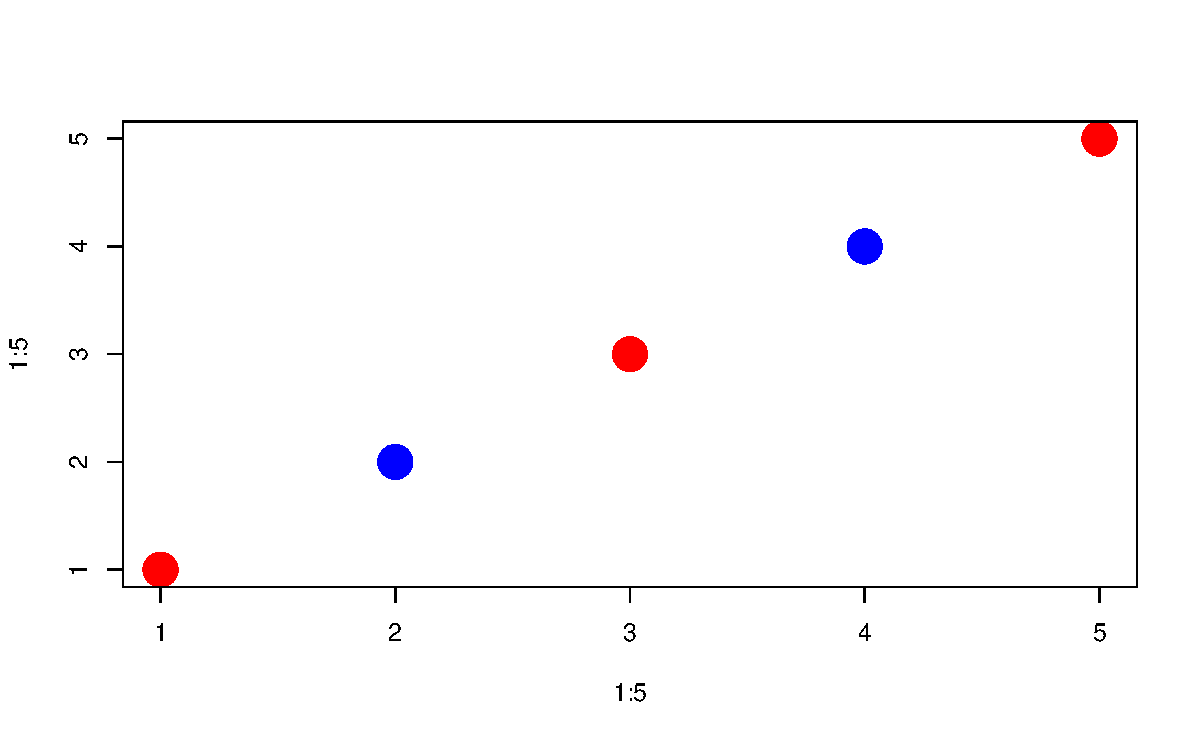
\includegraphics[width=0.7\linewidth]{DS4PS-I_files/figure-latex/unnamed-chunk-72-1} \end{center}

Here is an example of recycling gone wrong:

\begin{Shaded}
\begin{Highlighting}[]

\NormalTok{x1 <-}\StringTok{ }\KeywordTok{c}\NormalTok{(}\DecValTok{167}\NormalTok{,}\DecValTok{185}\NormalTok{,}\DecValTok{119}\NormalTok{,}\DecValTok{142}\NormalTok{)}

\NormalTok{x2 <-}\StringTok{ }\KeywordTok{c}\NormalTok{(}\StringTok{"adam"}\NormalTok{,}\StringTok{"jamal"}\NormalTok{,}\StringTok{"linda"}\NormalTok{,}\StringTok{"sriti"}\NormalTok{)}

\NormalTok{x3 <-}\StringTok{ }\KeywordTok{c}\NormalTok{(}\StringTok{"male"}\NormalTok{,}\StringTok{"male"}\NormalTok{,}\StringTok{"female"}\NormalTok{,}\StringTok{"female"}\NormalTok{)}

\NormalTok{x4 <-}\StringTok{ }\KeywordTok{c}\NormalTok{( }\StringTok{"treatment"}\NormalTok{,}\StringTok{"contro"}\NormalTok{,}\StringTok{"treatment"}\NormalTok{,}\StringTok{"control"}\NormalTok{ )}

\NormalTok{dat <-}\StringTok{ }\KeywordTok{data.frame}\NormalTok{( }\DataTypeTok{name=}\NormalTok{x2, }\DataTypeTok{sex=}\NormalTok{x3, }\DataTypeTok{treat=}\NormalTok{x4, }\DataTypeTok{strength=}\NormalTok{x1 )}


\CommentTok{# create a subset of data of all female study participants}

\NormalTok{dat}\OperatorTok{$}\NormalTok{sex }\OperatorTok{==}\StringTok{ "female"}
\CommentTok{### [1] FALSE FALSE  TRUE  TRUE}

\NormalTok{these <-}\StringTok{ }\NormalTok{dat}\OperatorTok{$}\NormalTok{sex }\OperatorTok{==}\StringTok{ "female"}

\NormalTok{dat[ these, ]  }\CommentTok{# correct subset}
\CommentTok{###    name    sex     treat strength}
\CommentTok{### 3 linda female treatment      119}
\CommentTok{### 4 sriti female   control      142}


\CommentTok{# same thing, but i mess is up - the female element is recycled in the overwrite}

\NormalTok{dat}\OperatorTok{$}\NormalTok{sex =}\StringTok{ "female"}    \CommentTok{# whoops just over-wrote my data! should be double equal}

\NormalTok{these <-}\StringTok{ }\NormalTok{dat}\OperatorTok{$}\NormalTok{sex }\OperatorTok{==}\StringTok{ "female"} 

\NormalTok{dat[ these , ]}
\CommentTok{###    name    sex     treat strength}
\CommentTok{### 1  adam female treatment      167}
\CommentTok{### 2 jamal female    contro      185}
\CommentTok{### 3 linda female treatment      119}
\CommentTok{### 4 sriti female   control      142}
\end{Highlighting}
\end{Shaded}

\hypertarget{missing-values-nas}{%
\section{Missing Values: NA's}\label{missing-values-nas}}

Missing values are coded differently in each data analysis program. SPSS
uses a period, for example. In R, missing values are coded as ``NA''.

The important thing to note is that R wants to make sure you know there
are missing values if you are conducting analysis. As a result, it will
give you the answer of ``NA'' when you try to do math with a vector that
includes a missing value. You have to ask it explicitly to ignore the
missing value.

\begin{Shaded}
\begin{Highlighting}[]
\NormalTok{x5 <-}\StringTok{ }\KeywordTok{c}\NormalTok{( }\DecValTok{1}\NormalTok{, }\DecValTok{2}\NormalTok{, }\DecValTok{3}\NormalTok{, }\DecValTok{4}\NormalTok{ )}

\NormalTok{x5}
\CommentTok{### [1] 1 2 3 4}

\KeywordTok{sum}\NormalTok{( x5 )}
\CommentTok{### [1] 10}

\KeywordTok{mean}\NormalTok{( x5 )}
\CommentTok{### [1] 2.5}

\NormalTok{x5 <-}\StringTok{ }\KeywordTok{c}\NormalTok{( }\DecValTok{1}\NormalTok{, }\DecValTok{2}\NormalTok{, }\OtherTok{NA}\NormalTok{, }\DecValTok{4}\NormalTok{ )}

\NormalTok{x5}
\CommentTok{### [1]  1  2 NA  4}

\CommentTok{# should missing values be treated as zeros or dropped? }

\KeywordTok{sum}\NormalTok{( x5 )}
\CommentTok{### [1] NA}

\KeywordTok{mean}\NormalTok{( x5 )}
\CommentTok{### [1] NA}

\KeywordTok{sum}\NormalTok{( x5, }\DataTypeTok{na.rm=}\NormalTok{T )   }\CommentTok{# na.rm=T argument drops missing values}
\CommentTok{### [1] 7}

\KeywordTok{mean}\NormalTok{( x5, }\DataTypeTok{na.rm=}\NormalTok{T )  }\CommentTok{# na.rm=T argument drops missing values}
\CommentTok{### [1] 2.333333}
\end{Highlighting}
\end{Shaded}

You cannot use the \emph{==} operator to identify missing values in a
dataset. There is a special \textbf{is.na()} function to locate all of
the missing values in a vector.

\begin{Shaded}
\begin{Highlighting}[]

\NormalTok{x5}
\CommentTok{### [1]  1  2 NA  4}

\NormalTok{x5 }\OperatorTok{==}\StringTok{ }\OtherTok{NA}    \CommentTok{# this does not do what you want}
\CommentTok{### [1] NA NA NA NA}

\KeywordTok{is.na}\NormalTok{( x5 )    }\CommentTok{# much better}
\CommentTok{### [1] FALSE FALSE  TRUE FALSE}

\OperatorTok{!}\StringTok{ }\KeywordTok{is.na}\NormalTok{( x5 )  }\CommentTok{# if you want to create a selector vector to drop missing values }
\CommentTok{### [1]  TRUE  TRUE FALSE  TRUE}

\NormalTok{x5[ }\OperatorTok{!}\StringTok{ }\KeywordTok{is.na}\NormalTok{(x5) ]}
\CommentTok{### [1] 1 2 4}

\NormalTok{x5[ }\KeywordTok{is.na}\NormalTok{(x5) ] <-}\StringTok{ }\DecValTok{0}  \CommentTok{# replace missing values with zero}
\end{Highlighting}
\end{Shaded}

\hypertarget{datasets}{%
\section{Datasets}\label{datasets}}

When we combine multiple vectors together, we now have a dataset. There
are three main types that we will use in this class.

\begin{longtable}[]{@{}ll@{}}
\toprule
Class & Description\tabularnewline
\midrule
\endhead
data frame & A typical data set comprised of several
variables\tabularnewline
matrix & A data set comprised of only numbers, used for matrix
math\tabularnewline
list & The grab bag of data structures - several vectors held
together\tabularnewline
\bottomrule
\end{longtable}

\hypertarget{data-frames}{%
\subsection{Data Frames}\label{data-frames}}

The most familiar spreadsheet-type data structure is called a data frame
in R. It consists of rows, which represent observations, and columns,
which represent variables.

\begin{Shaded}
\begin{Highlighting}[]

\KeywordTok{data}\NormalTok{( USArrests )}

\KeywordTok{dim}\NormalTok{( USArrests )   }\CommentTok{# number of rows by number of columns}
\CommentTok{### [1] 50  4}

\KeywordTok{names}\NormalTok{( USArrests )   }\CommentTok{# variable names or column names}
\CommentTok{### [1] "Murder"   "Assault"  "UrbanPop" "Rape"}

\KeywordTok{row.names}\NormalTok{( USArrests )}
\CommentTok{###  [1] "Alabama"        "Alaska"         "Arizona"        "Arkansas"      }
\CommentTok{###  [5] "California"     "Colorado"       "Connecticut"    "Delaware"      }
\CommentTok{###  [9] "Florida"        "Georgia"        "Hawaii"         "Idaho"         }
\CommentTok{### [13] "Illinois"       "Indiana"        "Iowa"           "Kansas"        }
\CommentTok{### [17] "Kentucky"       "Louisiana"      "Maine"          "Maryland"      }
\CommentTok{### [21] "Massachusetts"  "Michigan"       "Minnesota"      "Mississippi"   }
\CommentTok{### [25] "Missouri"       "Montana"        "Nebraska"       "Nevada"        }
\CommentTok{### [29] "New Hampshire"  "New Jersey"     "New Mexico"     "New York"      }
\CommentTok{### [33] "North Carolina" "North Dakota"   "Ohio"           "Oklahoma"      }
\CommentTok{### [37] "Oregon"         "Pennsylvania"   "Rhode Island"   "South Carolina"}
\CommentTok{### [41] "South Dakota"   "Tennessee"      "Texas"          "Utah"          }
\CommentTok{### [45] "Vermont"        "Virginia"       "Washington"     "West Virginia" }
\CommentTok{### [49] "Wisconsin"      "Wyoming"}

\KeywordTok{head}\NormalTok{( USArrests )  }\CommentTok{# print first six rows of the data}
\CommentTok{###            Murder Assault UrbanPop Rape}
\CommentTok{### Alabama      13.2     236       58 21.2}
\CommentTok{### Alaska       10.0     263       48 44.5}
\CommentTok{### Arizona       8.1     294       80 31.0}
\CommentTok{### Arkansas      8.8     190       50 19.5}
\CommentTok{### California    9.0     276       91 40.6}
\CommentTok{### Colorado      7.9     204       78 38.7}
\end{Highlighting}
\end{Shaded}

\hypertarget{matrices}{%
\subsection{Matrices}\label{matrices}}

A matrix is also a rectangular data object that consists of collections
of vectors, but it is special in the sense that it only has numeric
vectors and no variable names.

\begin{Shaded}
\begin{Highlighting}[]

\NormalTok{mat <-}\StringTok{ }\KeywordTok{matrix}\NormalTok{( }\DecValTok{1}\OperatorTok{:}\DecValTok{20}\NormalTok{, }\DataTypeTok{nrow=}\DecValTok{5}\NormalTok{ )}

\NormalTok{mat}
\CommentTok{###      [,1] [,2] [,3] [,4]}
\CommentTok{### [1,]    1    6   11   16}
\CommentTok{### [2,]    2    7   12   17}
\CommentTok{### [3,]    3    8   13   18}
\CommentTok{### [4,]    4    9   14   19}
\CommentTok{### [5,]    5   10   15   20}

\KeywordTok{names}\NormalTok{( mat )}
\CommentTok{### NULL}

\KeywordTok{dim}\NormalTok{( mat )}
\CommentTok{### [1] 5 4}

\KeywordTok{as.data.frame}\NormalTok{( mat )  }\CommentTok{# creates variable names}
\CommentTok{###   V1 V2 V3 V4}
\CommentTok{### 1  1  6 11 16}
\CommentTok{### 2  2  7 12 17}
\CommentTok{### 3  3  8 13 18}
\CommentTok{### 4  4  9 14 19}
\CommentTok{### 5  5 10 15 20}
\end{Highlighting}
\end{Shaded}

These are used almost exclusively for matrix algebra operations, which
are fundamental to mathematical statistics. We will not use matrices in
this course.

\hypertarget{lists}{%
\subsection{Lists}\label{lists}}

The list is the most flexible data structure. It is created by sticking
a bunch of unrelated vectors or datasets together. For example, when you
run a regression you generate a bunch of interesting information. This
information is saved as a list.

\begin{Shaded}
\begin{Highlighting}[]

\NormalTok{x <-}\StringTok{ }\DecValTok{1}\OperatorTok{:}\DecValTok{100}
\NormalTok{y <-}\StringTok{ }\DecValTok{2}\OperatorTok{*}\NormalTok{x }\OperatorTok{+}\StringTok{ }\KeywordTok{rnorm}\NormalTok{( }\DecValTok{100}\NormalTok{, }\DecValTok{0}\NormalTok{, }\DecValTok{10}\NormalTok{)}

\NormalTok{m}\FloatTok{.01}\NormalTok{ <-}\StringTok{ }\KeywordTok{lm}\NormalTok{( y }\OperatorTok{~}\StringTok{ }\NormalTok{x )}

\KeywordTok{names}\NormalTok{( m}\FloatTok{.01}\NormalTok{ )}
\CommentTok{###  [1] "coefficients"  "residuals"     "effects"       "rank"         }
\CommentTok{###  [5] "fitted.values" "assign"        "qr"            "df.residual"  }
\CommentTok{###  [9] "xlevels"       "call"          "terms"         "model"}

\NormalTok{m}\FloatTok{.01}\OperatorTok{$}\NormalTok{coefficients}
\CommentTok{### (Intercept)           x }
\CommentTok{###  -0.4693647   1.9900017}

\NormalTok{m}\FloatTok{.01}\OperatorTok{$}\NormalTok{residuals}
\CommentTok{###             1             2             3             4             5 }
\CommentTok{###  -5.550335387  -5.523043954  -2.397545001  -4.026392405  -9.786347652 }
\CommentTok{###             6             7             8             9            10 }
\CommentTok{###  -4.299829217  16.328838176  11.022620827   5.975011442  -7.860138374 }
\CommentTok{###            11            12            13            14            15 }
\CommentTok{### -19.084175623   5.409313437   6.049319845   0.314740675  12.235842348 }
\CommentTok{###            16            17            18            19            20 }
\CommentTok{###  -6.461082288 -14.135150772  -5.501481663  17.905437750   0.052597556 }
\CommentTok{###            21            22            23            24            25 }
\CommentTok{###   3.227863409  -9.045033608   5.533141805 -27.697685825  -1.051072540 }
\CommentTok{###            26            27            28            29            30 }
\CommentTok{###  -9.542730213  -7.386884572 -20.339122640   4.756852567   5.717793070 }
\CommentTok{###            31            32            33            34            35 }
\CommentTok{###  -2.239929737   1.001879835  -9.921130555  11.195671006  19.665299814 }
\CommentTok{###            36            37            38            39            40 }
\CommentTok{###  -0.002137996   8.551567078  12.788899550   6.778286572  17.811398915 }
\CommentTok{###            41            42            43            44            45 }
\CommentTok{###  -3.928598601   6.816672067  -8.576192387   4.916356938  24.086509503 }
\CommentTok{###            46            47            48            49            50 }
\CommentTok{###  -4.904712505   7.787847036  -4.387343645  11.585592478   2.825271120 }
\CommentTok{###            51            52            53            54            55 }
\CommentTok{### -14.637360099 -11.197067442   8.442867826   1.690803360   5.094803953 }
\CommentTok{###            56            57            58            59            60 }
\CommentTok{###   1.128606169   1.211005454 -12.265235061   4.827584234  -3.108942211 }
\CommentTok{###            61            62            63            64            65 }
\CommentTok{###  16.636337880   2.801215903  -1.174165114  -0.116690420   0.230620273 }
\CommentTok{###            66            67            68            69            70 }
\CommentTok{###  -8.578709617  -1.383561193  -6.039395088   5.133565734  17.893254198 }
\CommentTok{###            71            72            73            74            75 }
\CommentTok{###  -5.426680044  -4.070807741  -2.705410075   4.018599394 -13.665488760 }
\CommentTok{###            76            77            78            79            80 }
\CommentTok{###  -3.139886683   2.501396768  -6.041642807 -18.979281746   1.817114850 }
\CommentTok{###            81            82            83            84            85 }
\CommentTok{###  21.702075528   3.978804296  -8.587345385   4.792720487   3.309812058 }
\CommentTok{###            86            87            88            89            90 }
\CommentTok{### -11.969648741  -3.799179738  10.563989397  -0.981735969  -8.665395098 }
\CommentTok{###            91            92            93            94            95 }
\CommentTok{###   9.123964620  10.376745406  -8.079219567  -5.732294283   9.280406487 }
\CommentTok{###            96            97            98            99           100 }
\CommentTok{### -14.297224926  -4.321746578  -8.965102686 -14.908978709  19.589373845}

\NormalTok{m}\FloatTok{.01}\OperatorTok{$}\NormalTok{call}
\CommentTok{### lm(formula = y ~ x)}
\end{Highlighting}
\end{Shaded}

These output are all related to the model we have run, so they are kept
organized by the list so they can be used for various further steps like
comparing models or checking for model fit.

A data frame is a bit more rigid that a list in that you cannot combine
elements that do not have the same dimsions.

\begin{Shaded}
\begin{Highlighting}[]

\CommentTok{# new.dataframe <- data.frame( m.01$coefficients, m.01$residuals, m.01$call )}
\CommentTok{#}
\CommentTok{# these will fail because the vectors have different lengths }
\end{Highlighting}
\end{Shaded}

\hypertarget{the-attach-function}{%
\section{The `attach' Function}\label{the-attach-function}}

\textbf{Never Use This!}

This is a convenient function for making variable names easily
accessible, but it is problematic because of:

scope

conflicting variable names

\begin{Shaded}
\begin{Highlighting}[]

\NormalTok{x <-}\StringTok{ }\DecValTok{1}\OperatorTok{:}\DecValTok{5}
\NormalTok{y <-}\StringTok{ }\DecValTok{6}\OperatorTok{:}\DecValTok{10}

\NormalTok{dat <-}\StringTok{ }\KeywordTok{data.frame}\NormalTok{(x,y)}

\KeywordTok{rm}\NormalTok{(x)}
\KeywordTok{rm}\NormalTok{(y)}


\CommentTok{# I want to transform x in my dataset}

\KeywordTok{attach}\NormalTok{( dat )}

\DecValTok{2}\OperatorTok{*}\NormalTok{x}
\CommentTok{### [1]  2  4  6  8 10}

\NormalTok{x <-}\StringTok{ }\DecValTok{2}\OperatorTok{*}\NormalTok{x}

\KeywordTok{detach}\NormalTok{( dat )}

\NormalTok{x}
\CommentTok{### [1]  2  4  6  8 10}

\NormalTok{dat  }\CommentTok{# whoops! I didn't save my work in the dataset}
\CommentTok{###   x  y}
\CommentTok{### 1 1  6}
\CommentTok{### 2 2  7}
\CommentTok{### 3 3  8}
\CommentTok{### 4 4  9}
\CommentTok{### 5 5 10}
\end{Highlighting}
\end{Shaded}

You will see the \textbf{attach()} function used on occassion, and it is
tempting because you can write the variable names directly. But in
general, try to avoid the \textbf{attach()} function and don't form bad
habits by using it now because when your scripts become more complicated
then can cause problmes.

\hypertarget{logical-statements}{%
\chapter{Logical Statements}\label{logical-statements}}

\hypertarget{key-concepts-2}{%
\section{Key Concepts}\label{key-concepts-2}}

\begin{figure}

{\centering 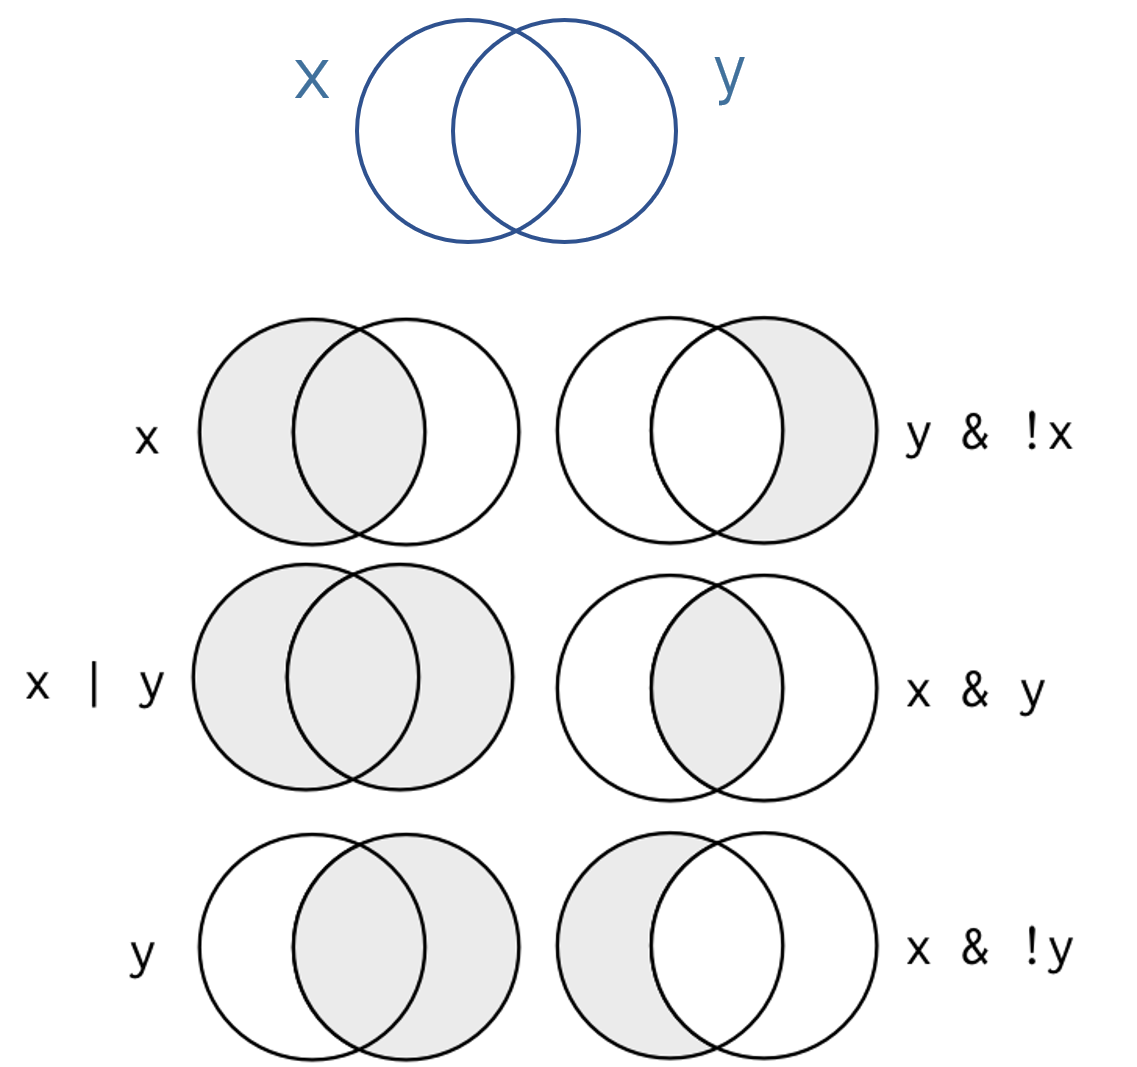
\includegraphics[width=0.7\linewidth]{figures/set_theory} 

}

\caption{Logical statements define group membership}\label{fig:unnamed-chunk-83}
\end{figure}

\hypertarget{operators}{%
\section{Operators}\label{operators}}

Logical operators are the most basic type of data programming and the
core of many types of data analysis. Most of the time we are not
conducting fancy statistics, we just want to identify members of a group
(print all of the females from the study), or describe things that
belong to a subset of the data (compare the average price of houses with
garages to houses without garages).

In order to accomplish these simple tasks we need to use logic
statements. A logic statement answers the question, does an observation
belong to a group.

Many times groups are simple. Show me all of the professions that make
over \$100k a year, for example.

Sometimes groups are complex. Identify the African American children
from a specific zip code in Chicago that live in households with single
mothers.

You will use nine basic logical operators:

\begin{longtable}[]{@{}ll@{}}
\toprule
Operator & Description\tabularnewline
\midrule
\endhead
\textless{} & less than\tabularnewline
\textless{}= & less than or equal to\tabularnewline
\textgreater{} & greater than\tabularnewline
\textgreater{}= & greater than or equal to\tabularnewline
== & exactly equal to\tabularnewline
!= & not equal to\tabularnewline
x \textbar{} y & x OR y\tabularnewline
x \& y & x AND y\tabularnewline
! & opposite of\tabularnewline
\bottomrule
\end{longtable}

Logical operators create logical vectors, a vector that contains only
TRUE or FALSE. The TRUE means that the observation belongs to the group,
FALSE means it does not.

\begin{Shaded}
\begin{Highlighting}[]
\NormalTok{x1 <-}\StringTok{ }\KeywordTok{c}\NormalTok{( }\DecValTok{7}\NormalTok{, }\DecValTok{9}\NormalTok{, }\DecValTok{1}\NormalTok{, }\DecValTok{2}\NormalTok{ )}

\NormalTok{x1 }\OperatorTok{>}\StringTok{ }\DecValTok{7}
\CommentTok{### [1] FALSE  TRUE FALSE FALSE}

\NormalTok{x1 }\OperatorTok{>=}\StringTok{ }\DecValTok{7}
\CommentTok{### [1]  TRUE  TRUE FALSE FALSE}

\NormalTok{x1 }\OperatorTok{==}\StringTok{ }\DecValTok{9}
\CommentTok{### [1] FALSE  TRUE FALSE FALSE}

\NormalTok{x1 =}\StringTok{ }\DecValTok{9}  \CommentTok{# don't use a single equals operator!  it overwrites your variable}

\NormalTok{x1}
\CommentTok{### [1] 9}

\NormalTok{x1 <-}\StringTok{ }\KeywordTok{c}\NormalTok{(}\DecValTok{7}\NormalTok{,}\DecValTok{9}\NormalTok{,}\DecValTok{1}\NormalTok{,}\DecValTok{2}\NormalTok{)}

\NormalTok{x1 }\OperatorTok{==}\StringTok{ }\DecValTok{9} \OperatorTok{|}\StringTok{ }\NormalTok{x1 }\OperatorTok{==}\StringTok{ }\DecValTok{1}
\CommentTok{### [1] FALSE  TRUE  TRUE FALSE}


\NormalTok{x2 <-}\StringTok{ }\KeywordTok{c}\NormalTok{(}\StringTok{"male"}\NormalTok{,}\StringTok{"male"}\NormalTok{,}\StringTok{"female"}\NormalTok{,}\StringTok{"female"}\NormalTok{)}

\NormalTok{x3 <-}\StringTok{ }\KeywordTok{c}\NormalTok{(}\StringTok{"treatment"}\NormalTok{,}\StringTok{"control"}\NormalTok{,}\StringTok{"treatment"}\NormalTok{,}\StringTok{"control"}\NormalTok{)}

\CommentTok{# x2 == male  # this will not work because male is not enclosed with quotes}

\NormalTok{x2 }\OperatorTok{==}\StringTok{ "female"}
\CommentTok{### [1] FALSE FALSE  TRUE  TRUE}

\NormalTok{x2 }\OperatorTok{==}\StringTok{ "female"} \OperatorTok{&}\StringTok{ }\NormalTok{x3 }\OperatorTok{==}\StringTok{ "treatment"}
\CommentTok{### [1] FALSE FALSE  TRUE FALSE}
\end{Highlighting}
\end{Shaded}

Note that we use operators to create logical vectors where TRUE
designates observation that belong to the defined group, and FALSE
designates observations outside the group. We use these logical vectors
in three ways:

\textbf{ONE:} We can create a selector variable that is used for
subsets. When a logical vector is passed to the subset function it will
keep all observations with a TRUE value, and drop observations with a
FALSE value.

\begin{Shaded}
\begin{Highlighting}[]

\NormalTok{x1}
\CommentTok{### [1] 7 9 1 2}

\NormalTok{x1 }\OperatorTok{>}\StringTok{ }\DecValTok{5}
\CommentTok{### [1]  TRUE  TRUE FALSE FALSE}

\NormalTok{keep.these <-}\StringTok{ }\NormalTok{x1 }\OperatorTok{>}\StringTok{ }\DecValTok{5}

\NormalTok{x1[ keep.these ]}
\CommentTok{### [1] 7 9}

\CommentTok{# you can create a selector variable with one variable, and apply it to another}

\NormalTok{x2[ keep.these ]  }\CommentTok{# sex of observations where x1 > 5}
\CommentTok{### [1] "male" "male"}
\end{Highlighting}
\end{Shaded}

\textbf{TWO}: Logical vectors give us an easy way to count things within
defined groups.

We can apply a \textbf{sum()} function to a logical vector, and the
result will be a tally of all of the TRUE cases.

\begin{Shaded}
\begin{Highlighting}[]

\CommentTok{# how many females do we have in our study?}

\KeywordTok{sum}\NormalTok{( x2 }\OperatorTok{==}\StringTok{ "female"}\NormalTok{ )}
\CommentTok{### [1] 2}

\CommentTok{# how many females do we have in our treatment group?}

\KeywordTok{sum}\NormalTok{( x2 }\OperatorTok{==}\StringTok{ "female"} \OperatorTok{&}\StringTok{ }\NormalTok{x3 }\OperatorTok{==}\StringTok{ "treatment"}\NormalTok{ )}
\CommentTok{### [1] 1}
\end{Highlighting}
\end{Shaded}

\textbf{THREE}: We use selector variables to replace observations with
new values using the assignment operator. This is similar to a find and
replace operation.

\begin{Shaded}
\begin{Highlighting}[]

\NormalTok{x7 <-}\StringTok{ }\KeywordTok{c}\NormalTok{( }\StringTok{"mole"}\NormalTok{,}\StringTok{"mouse"}\NormalTok{,}\StringTok{"shrew"}\NormalTok{,}\StringTok{"mouse"}\NormalTok{,}\StringTok{"rat"}\NormalTok{,}\StringTok{"shrew"}\NormalTok{)}

\CommentTok{# the lab assistant incorrectly identified the shrews}

\NormalTok{x7}
\CommentTok{### [1] "mole"  "mouse" "shrew" "mouse" "rat"   "shrew"}

\NormalTok{x7[ x7 }\OperatorTok{==}\StringTok{ "shrew"}\NormalTok{ ] <-}\StringTok{ "possum"}

\NormalTok{x7}
\CommentTok{### [1] "mole"   "mouse"  "possum" "mouse"  "rat"    "possum"}


\CommentTok{# we don't know if linda received the treatment}

\NormalTok{x3 <-}\StringTok{ }\KeywordTok{c}\NormalTok{(}\StringTok{"adam"}\NormalTok{,}\StringTok{"jamal"}\NormalTok{,}\StringTok{"linda"}\NormalTok{,}\StringTok{"sriti"}\NormalTok{)}

\NormalTok{x4 <-}\StringTok{ }\KeywordTok{c}\NormalTok{( }\StringTok{"treatment"}\NormalTok{,}\StringTok{"control"}\NormalTok{,}\StringTok{"treatment"}\NormalTok{,}\StringTok{"control"}\NormalTok{)}

\NormalTok{x4[ x3 }\OperatorTok{==}\StringTok{ "linda"}\NormalTok{ ] <-}\StringTok{ }\OtherTok{NA}

\NormalTok{x4}
\CommentTok{### [1] "treatment" "control"   NA          "control"}
\end{Highlighting}
\end{Shaded}

The \textbf{!} operator is a special case, where it is not used to
define a new logical vector, but rather it swaps the values of an
existing logical vector.

\begin{Shaded}
\begin{Highlighting}[]

\NormalTok{x1}
\CommentTok{### [1] 7 9 1 2}

\NormalTok{these <-}\StringTok{ }\NormalTok{x1 }\OperatorTok{>}\StringTok{ }\DecValTok{5}

\NormalTok{these}
\CommentTok{### [1]  TRUE  TRUE FALSE FALSE}

\OperatorTok{!}\StringTok{ }\NormalTok{these}
\CommentTok{### [1] FALSE FALSE  TRUE  TRUE}

\OperatorTok{!}\StringTok{ }\OtherTok{TRUE}
\CommentTok{### [1] FALSE}

\OperatorTok{!}\StringTok{ }\OtherTok{FALSE}
\CommentTok{### [1] TRUE}
\end{Highlighting}
\end{Shaded}

\hypertarget{logical-vectors}{%
\section{Logical Vectors}\label{logical-vectors}}

Logical vectors are collections of a set of TRUE and FALSE statements.

Logical statements allow us to define groups based upon criteria, then
decide whether observations belong to the group. A logical statement is
one that contains a logical operator, and returns only TRUE, FALSE, or
NA values.

Logical vectors are important because organizing data into these sets is
what drives all of the advanced data analytics (set theory is at the
basis of mathematics and computer science).

\begin{longtable}[]{@{}cccc@{}}
\toprule
\begin{minipage}[b]{0.10\columnwidth}\centering
name\strut
\end{minipage} & \begin{minipage}[b]{0.11\columnwidth}\centering
sex\strut
\end{minipage} & \begin{minipage}[b]{0.15\columnwidth}\centering
treat\strut
\end{minipage} & \begin{minipage}[b]{0.15\columnwidth}\centering
strength\strut
\end{minipage}\tabularnewline
\midrule
\endhead
\begin{minipage}[t]{0.10\columnwidth}\centering
adam\strut
\end{minipage} & \begin{minipage}[t]{0.11\columnwidth}\centering
male\strut
\end{minipage} & \begin{minipage}[t]{0.15\columnwidth}\centering
treatment\strut
\end{minipage} & \begin{minipage}[t]{0.15\columnwidth}\centering
167\strut
\end{minipage}\tabularnewline
\begin{minipage}[t]{0.10\columnwidth}\centering
jamal\strut
\end{minipage} & \begin{minipage}[t]{0.11\columnwidth}\centering
male\strut
\end{minipage} & \begin{minipage}[t]{0.15\columnwidth}\centering
control\strut
\end{minipage} & \begin{minipage}[t]{0.15\columnwidth}\centering
185\strut
\end{minipage}\tabularnewline
\begin{minipage}[t]{0.10\columnwidth}\centering
linda\strut
\end{minipage} & \begin{minipage}[t]{0.11\columnwidth}\centering
female\strut
\end{minipage} & \begin{minipage}[t]{0.15\columnwidth}\centering
treatment\strut
\end{minipage} & \begin{minipage}[t]{0.15\columnwidth}\centering
119\strut
\end{minipage}\tabularnewline
\begin{minipage}[t]{0.10\columnwidth}\centering
sriti\strut
\end{minipage} & \begin{minipage}[t]{0.11\columnwidth}\centering
female\strut
\end{minipage} & \begin{minipage}[t]{0.15\columnwidth}\centering
control\strut
\end{minipage} & \begin{minipage}[t]{0.15\columnwidth}\centering
142\strut
\end{minipage}\tabularnewline
\bottomrule
\end{longtable}

\begin{Shaded}
\begin{Highlighting}[]
\NormalTok{dat}\OperatorTok{$}\NormalTok{name }\OperatorTok{==}\StringTok{ "sriti"}
\CommentTok{### [1] FALSE FALSE FALSE  TRUE}

\NormalTok{dat}\OperatorTok{$}\NormalTok{sex }\OperatorTok{==}\StringTok{ "male"}
\CommentTok{### [1]  TRUE  TRUE FALSE FALSE}

\NormalTok{dat}\OperatorTok{$}\NormalTok{strength }\OperatorTok{>}\StringTok{ }\DecValTok{180}
\CommentTok{### [1] FALSE  TRUE FALSE FALSE}
\end{Highlighting}
\end{Shaded}

When defining logical vectors, you can use the abbreviated versions of T
for TRUE and F for FALSE.

\begin{Shaded}
\begin{Highlighting}[]
\NormalTok{z1 <-}\StringTok{ }\KeywordTok{c}\NormalTok{(T,T,F,T,F,F)}
\NormalTok{z1}
\CommentTok{### [1]  TRUE  TRUE FALSE  TRUE FALSE FALSE}
\end{Highlighting}
\end{Shaded}

Typically logical vectors are used in combination with subset operators
to identify specific groups in the data.

\begin{Shaded}
\begin{Highlighting}[]
\CommentTok{# isolate data on all of the females in the dataset}
\NormalTok{dat[ dat}\OperatorTok{$}\NormalTok{sex }\OperatorTok{==}\StringTok{ "female"}\NormalTok{ , ]}
\CommentTok{###    name    sex     treat strength}
\CommentTok{### 3 linda female treatment      119}
\CommentTok{### 4 sriti female   control      142}
\end{Highlighting}
\end{Shaded}

Note how NAs affect compound logical statements:

\begin{Shaded}
\begin{Highlighting}[]
\OtherTok{TRUE} \OperatorTok{&}\StringTok{ }\OtherTok{TRUE}
\CommentTok{### [1] TRUE}

\OtherTok{TRUE} \OperatorTok{&}\StringTok{ }\OtherTok{FALSE}
\CommentTok{### [1] FALSE}

\OtherTok{TRUE} \OperatorTok{&}\StringTok{ }\OtherTok{NA}
\CommentTok{### [1] NA}

\OtherTok{FALSE} \OperatorTok{&}\StringTok{ }\OtherTok{NA}
\CommentTok{### [1] FALSE}
\end{Highlighting}
\end{Shaded}

If one condition is FALSE and the other is NA, the missing value does
not matter in this case because under the \& condition both must be TRUE
for the observation to belong to the group we are defining with the
logical statement, so it should be excluded even if we don't know the
value for the second condition. For example, if we want to select all
women in the treatment group, then a man is excluded from the group,
even if it is unclear whether he belongs to the treatment or control
condition.

On the other hand, if one condition is TRUE, and another is NA, R does
not want to throw out the data because the state of the missing value is
unclear. As a result, it will preserve the observation, but it will
replace all of the data with missing values.

\begin{longtable}[]{@{}cccc@{}}
\toprule
\begin{minipage}[b]{0.10\columnwidth}\centering
name\strut
\end{minipage} & \begin{minipage}[b]{0.11\columnwidth}\centering
sex\strut
\end{minipage} & \begin{minipage}[b]{0.15\columnwidth}\centering
treat\strut
\end{minipage} & \begin{minipage}[b]{0.15\columnwidth}\centering
strength\strut
\end{minipage}\tabularnewline
\midrule
\endhead
\begin{minipage}[t]{0.10\columnwidth}\centering
adam\strut
\end{minipage} & \begin{minipage}[t]{0.11\columnwidth}\centering
male\strut
\end{minipage} & \begin{minipage}[t]{0.15\columnwidth}\centering
treatment\strut
\end{minipage} & \begin{minipage}[t]{0.15\columnwidth}\centering
167\strut
\end{minipage}\tabularnewline
\begin{minipage}[t]{0.10\columnwidth}\centering
jamal\strut
\end{minipage} & \begin{minipage}[t]{0.11\columnwidth}\centering
male\strut
\end{minipage} & \begin{minipage}[t]{0.15\columnwidth}\centering
control\strut
\end{minipage} & \begin{minipage}[t]{0.15\columnwidth}\centering
185\strut
\end{minipage}\tabularnewline
\begin{minipage}[t]{0.10\columnwidth}\centering
linda\strut
\end{minipage} & \begin{minipage}[t]{0.11\columnwidth}\centering
female\strut
\end{minipage} & \begin{minipage}[t]{0.15\columnwidth}\centering
treatment\strut
\end{minipage} & \begin{minipage}[t]{0.15\columnwidth}\centering
119\strut
\end{minipage}\tabularnewline
\begin{minipage}[t]{0.10\columnwidth}\centering
sriti\strut
\end{minipage} & \begin{minipage}[t]{0.11\columnwidth}\centering
female\strut
\end{minipage} & \begin{minipage}[t]{0.15\columnwidth}\centering
control\strut
\end{minipage} & \begin{minipage}[t]{0.15\columnwidth}\centering
142\strut
\end{minipage}\tabularnewline
\bottomrule
\end{longtable}

\begin{Shaded}
\begin{Highlighting}[]
\NormalTok{keep.these <-}\StringTok{ }\KeywordTok{c}\NormalTok{(T,F,}\OtherTok{NA}\NormalTok{,F)}
\NormalTok{dat[ keep.these , ]}
\CommentTok{###    name  sex     treat strength}
\CommentTok{### 1  adam male treatment      167}
\CommentTok{### NA <NA> <NA>      <NA>       NA}
\end{Highlighting}
\end{Shaded}

To remove these rows with missing values in your selector vector,
replace all NAs with FALSE:

\begin{Shaded}
\begin{Highlighting}[]
\NormalTok{keep.these[ }\KeywordTok{is.na}\NormalTok{(keep.these) ] <-}\StringTok{ }\OtherTok{FALSE}
\NormalTok{dat[ keep.these , ]}
\CommentTok{###   name  sex     treat strength}
\CommentTok{### 1 adam male treatment      167}
\end{Highlighting}
\end{Shaded}

\hypertarget{subsets}{%
\section{Subsets}\label{subsets}}

The subset operators \textbf{{[} {]}} are one of the most common you
will use in R.

The primary rule of subsets is to use a data operator to create a
logical selector vector, and use that to generate subsets. Any
observation that corresponds to TRUE will be retained, any observation
that corresponds to FALSE will be dropped.

For vectors, you need to specify a single dimension.

\begin{Shaded}
\begin{Highlighting}[]
\NormalTok{these <-}\StringTok{ }\NormalTok{x1 }\OperatorTok{>}\StringTok{ }\DecValTok{140}     \CommentTok{# selector vector}

\NormalTok{these}
\CommentTok{### [1] FALSE FALSE FALSE FALSE}

\NormalTok{x1[ these ]}
\CommentTok{### numeric(0)}

\NormalTok{x2[ these ]}
\CommentTok{### character(0)}
\end{Highlighting}
\end{Shaded}

For data frames, you need two dimensions (rows and columns). The two
dimensions are seperated by a comma, and if you leave one blank you will
not drop anything.

\begin{quote}
dat{[} row position , column position {]}
\end{quote}

\begin{longtable}[]{@{}cccc@{}}
\toprule
\begin{minipage}[b]{0.10\columnwidth}\centering
name\strut
\end{minipage} & \begin{minipage}[b]{0.11\columnwidth}\centering
sex\strut
\end{minipage} & \begin{minipage}[b]{0.15\columnwidth}\centering
treat\strut
\end{minipage} & \begin{minipage}[b]{0.15\columnwidth}\centering
strength\strut
\end{minipage}\tabularnewline
\midrule
\endhead
\begin{minipage}[t]{0.10\columnwidth}\centering
adam\strut
\end{minipage} & \begin{minipage}[t]{0.11\columnwidth}\centering
male\strut
\end{minipage} & \begin{minipage}[t]{0.15\columnwidth}\centering
treatment\strut
\end{minipage} & \begin{minipage}[t]{0.15\columnwidth}\centering
167\strut
\end{minipage}\tabularnewline
\begin{minipage}[t]{0.10\columnwidth}\centering
jamal\strut
\end{minipage} & \begin{minipage}[t]{0.11\columnwidth}\centering
male\strut
\end{minipage} & \begin{minipage}[t]{0.15\columnwidth}\centering
control\strut
\end{minipage} & \begin{minipage}[t]{0.15\columnwidth}\centering
185\strut
\end{minipage}\tabularnewline
\begin{minipage}[t]{0.10\columnwidth}\centering
linda\strut
\end{minipage} & \begin{minipage}[t]{0.11\columnwidth}\centering
female\strut
\end{minipage} & \begin{minipage}[t]{0.15\columnwidth}\centering
treatment\strut
\end{minipage} & \begin{minipage}[t]{0.15\columnwidth}\centering
119\strut
\end{minipage}\tabularnewline
\begin{minipage}[t]{0.10\columnwidth}\centering
sriti\strut
\end{minipage} & \begin{minipage}[t]{0.11\columnwidth}\centering
female\strut
\end{minipage} & \begin{minipage}[t]{0.15\columnwidth}\centering
control\strut
\end{minipage} & \begin{minipage}[t]{0.15\columnwidth}\centering
142\strut
\end{minipage}\tabularnewline
\bottomrule
\end{longtable}

\begin{Shaded}
\begin{Highlighting}[]
\NormalTok{these <-}\StringTok{ }\NormalTok{dat}\OperatorTok{$}\NormalTok{treat }\OperatorTok{==}\StringTok{ "treatment"}

\NormalTok{dat[ these , ]   }\CommentTok{# all data in the treatment group}
\CommentTok{###    name    sex     treat strength}
\CommentTok{### 1  adam   male treatment      167}
\CommentTok{### 3 linda female treatment      119}

\NormalTok{dat[ , }\KeywordTok{c}\NormalTok{(}\StringTok{"name"}\NormalTok{,}\StringTok{"sex"}\NormalTok{) ]  }\CommentTok{# select two columns of data}
\CommentTok{###    name    sex}
\CommentTok{### 1  adam   male}
\CommentTok{### 2 jamal   male}
\CommentTok{### 3 linda female}
\CommentTok{### 4 sriti female}

\CommentTok{# to keep a subset as a separate dataset}

\NormalTok{dat.women <-}\StringTok{ }\NormalTok{dat[ dat}\OperatorTok{$}\NormalTok{sex }\OperatorTok{==}\StringTok{ "female"}\NormalTok{ , ]}

\NormalTok{dat.women}
\CommentTok{###    name    sex     treat strength}
\CommentTok{### 3 linda female treatment      119}
\CommentTok{### 4 sriti female   control      142}
\end{Highlighting}
\end{Shaded}

Note the rules listed above about subsetting factors. After applying a
subset, they will retain all of the original levels, even when they are
not longer useful. You need to drop the unused levels if you would like
them to be omitted from functions that use the factor levels for
analysis.

\begin{Shaded}
\begin{Highlighting}[]

\NormalTok{df <-}\StringTok{ }\KeywordTok{data.frame}\NormalTok{( }\DataTypeTok{letters=}\NormalTok{LETTERS[}\DecValTok{1}\OperatorTok{:}\DecValTok{5}\NormalTok{], }\DataTypeTok{numbers=}\KeywordTok{seq}\NormalTok{(}\DecValTok{1}\OperatorTok{:}\DecValTok{5}\NormalTok{) )}

\KeywordTok{levels}\NormalTok{( df}\OperatorTok{$}\NormalTok{letters )}
\CommentTok{### [1] "A" "B" "C" "D" "E"}

\NormalTok{sub.df <-}\StringTok{ }\NormalTok{df[ }\DecValTok{1}\OperatorTok{:}\DecValTok{3}\NormalTok{, ]}

\NormalTok{sub.df}\OperatorTok{$}\NormalTok{letters}
\CommentTok{### [1] A B C}
\CommentTok{### Levels: A B C D E}

\KeywordTok{levels}\NormalTok{( sub.df}\OperatorTok{$}\NormalTok{letters )}
\CommentTok{### [1] "A" "B" "C" "D" "E"}

\KeywordTok{droplevels}\NormalTok{( sub.df}\OperatorTok{$}\NormalTok{letters )}
\CommentTok{### [1] A B C}
\CommentTok{### Levels: A B C}

\NormalTok{sub.df}\OperatorTok{$}\NormalTok{letters <-}\StringTok{ }\KeywordTok{droplevels}\NormalTok{( sub.df}\OperatorTok{$}\NormalTok{letters )}
\end{Highlighting}
\end{Shaded}

\hypertarget{part-part-ii-data-wrangling}{%
\part{PART II: DATA
WRANGLING}\label{part-part-ii-data-wrangling}}

\hypertarget{merging-data}{%
\chapter{Merging Data}\label{merging-data}}

\hypertarget{packages-used-in-this-chapter}{%
\section{Packages Used in This
Chapter}\label{packages-used-in-this-chapter}}

\begin{Shaded}
\begin{Highlighting}[]
\KeywordTok{library}\NormalTok{( pander )}
\KeywordTok{library}\NormalTok{( dplyr )}
\KeywordTok{library}\NormalTok{( maps )}
\end{Highlighting}
\end{Shaded}

\hypertarget{relational-databases}{%
\section{Relational Databases}\label{relational-databases}}

Modern databases are huge - think about the amount of information stored
at Amazon in the history of each transation, the database where Google
logs every single search from every person around the world, or
Twitter's database of all of the tweets (millions each day).

When databases become large, flat spreadsheet style formats are not
useful because they create a lot of redundant information, are large to
store, and are not efficient to search. Large datasets are instead
stored in relational databases - sets of tables that contain unique IDs
that allow them to be joined when necessary.

For example, consider a simple customer database. We don't want to store
customer info with our transactions because we would be repeating their
name and street address every time they make a new purchase. As a
result, we store customer information and transaction information
separately.

\textbf{Customer Database}

\begin{longtable}[]{@{}ccccc@{}}
\toprule
\begin{minipage}[b]{0.17\columnwidth}\centering
CUSTOMER.ID\strut
\end{minipage} & \begin{minipage}[b]{0.16\columnwidth}\centering
FIRST.NAME\strut
\end{minipage} & \begin{minipage}[b]{0.14\columnwidth}\centering
LAST.NAME\strut
\end{minipage} & \begin{minipage}[b]{0.19\columnwidth}\centering
ADDRESS\strut
\end{minipage} & \begin{minipage}[b]{0.13\columnwidth}\centering
ZIP.CODE\strut
\end{minipage}\tabularnewline
\midrule
\endhead
\begin{minipage}[t]{0.17\columnwidth}\centering
178\strut
\end{minipage} & \begin{minipage}[t]{0.16\columnwidth}\centering
Alvaro\strut
\end{minipage} & \begin{minipage}[t]{0.14\columnwidth}\centering
Jaurez\strut
\end{minipage} & \begin{minipage}[t]{0.19\columnwidth}\centering
123 Park Ave\strut
\end{minipage} & \begin{minipage}[t]{0.13\columnwidth}\centering
57701\strut
\end{minipage}\tabularnewline
\begin{minipage}[t]{0.17\columnwidth}\centering
934\strut
\end{minipage} & \begin{minipage}[t]{0.16\columnwidth}\centering
Janette\strut
\end{minipage} & \begin{minipage}[t]{0.14\columnwidth}\centering
Johnson\strut
\end{minipage} & \begin{minipage}[t]{0.19\columnwidth}\centering
456 Candy Ln\strut
\end{minipage} & \begin{minipage}[t]{0.13\columnwidth}\centering
57701\strut
\end{minipage}\tabularnewline
\begin{minipage}[t]{0.17\columnwidth}\centering
269\strut
\end{minipage} & \begin{minipage}[t]{0.16\columnwidth}\centering
Latisha\strut
\end{minipage} & \begin{minipage}[t]{0.14\columnwidth}\centering
Shane\strut
\end{minipage} & \begin{minipage}[t]{0.19\columnwidth}\centering
1600 Penn Ave\strut
\end{minipage} & \begin{minipage}[t]{0.13\columnwidth}\centering
20500\strut
\end{minipage}\tabularnewline
\bottomrule
\end{longtable}

\textbf{Transactions Database}

\begin{longtable}[]{@{}ccc@{}}
\toprule
\begin{minipage}[b]{0.18\columnwidth}\centering
CUSTOMER.ID\strut
\end{minipage} & \begin{minipage}[b]{0.13\columnwidth}\centering
PRODUCT\strut
\end{minipage} & \begin{minipage}[b]{0.13\columnwidth}\centering
PRICE\strut
\end{minipage}\tabularnewline
\midrule
\endhead
\begin{minipage}[t]{0.18\columnwidth}\centering
178\strut
\end{minipage} & \begin{minipage}[t]{0.13\columnwidth}\centering
video\strut
\end{minipage} & \begin{minipage}[t]{0.13\columnwidth}\centering
5.38\strut
\end{minipage}\tabularnewline
\begin{minipage}[t]{0.18\columnwidth}\centering
178\strut
\end{minipage} & \begin{minipage}[t]{0.13\columnwidth}\centering
shovel\strut
\end{minipage} & \begin{minipage}[t]{0.13\columnwidth}\centering
12\strut
\end{minipage}\tabularnewline
\begin{minipage}[t]{0.18\columnwidth}\centering
269\strut
\end{minipage} & \begin{minipage}[t]{0.13\columnwidth}\centering
book\strut
\end{minipage} & \begin{minipage}[t]{0.13\columnwidth}\centering
3.99\strut
\end{minipage}\tabularnewline
\begin{minipage}[t]{0.18\columnwidth}\centering
269\strut
\end{minipage} & \begin{minipage}[t]{0.13\columnwidth}\centering
purse\strut
\end{minipage} & \begin{minipage}[t]{0.13\columnwidth}\centering
8\strut
\end{minipage}\tabularnewline
\begin{minipage}[t]{0.18\columnwidth}\centering
934\strut
\end{minipage} & \begin{minipage}[t]{0.13\columnwidth}\centering
mirror\strut
\end{minipage} & \begin{minipage}[t]{0.13\columnwidth}\centering
7.64\strut
\end{minipage}\tabularnewline
\bottomrule
\end{longtable}

If we want to make the information actionable then we need to combine
these datasets. For example, perhaps we want to know the average
purchase amount from an individual in the 57701 zip code. We cannot
answer that question with either dataset since the zip code is in one
dataset, and the price is in another. We need to merge the data.

\begin{Shaded}
\begin{Highlighting}[]

\KeywordTok{merge}\NormalTok{( customer.info, purchases )   }
\CommentTok{###   CUSTOMER.ID FIRST.NAME LAST.NAME       ADDRESS ZIP.CODE PRODUCT PRICE}
\CommentTok{### 1         178     Alvaro    Jaurez  123 Park Ave    57701   video  5.38}
\CommentTok{### 2         178     Alvaro    Jaurez  123 Park Ave    57701  shovel 12.00}
\CommentTok{### 3         269    Latisha     Shane 1600 Penn Ave    20500    book  3.99}
\CommentTok{### 4         269    Latisha     Shane 1600 Penn Ave    20500   purse  8.00}
\CommentTok{### 5         934    Janette   Johnson  456 Candy Ln    57701  mirror  7.64}

\NormalTok{full.dat <-}\StringTok{ }\KeywordTok{merge}\NormalTok{( customer.info, purchases ) }

\NormalTok{full.dat}\OperatorTok{$}\NormalTok{PRICE[ full.dat}\OperatorTok{$}\NormalTok{ZIP.CODE }\OperatorTok{==}\StringTok{ "57701"}\NormalTok{ ]}
\CommentTok{### [1]  5.38 12.00  7.64}

\KeywordTok{mean}\NormalTok{( full.dat}\OperatorTok{$}\NormalTok{PRICE[ full.dat}\OperatorTok{$}\NormalTok{ZIP.CODE }\OperatorTok{==}\StringTok{ "57701"}\NormalTok{ ] )}
\CommentTok{### [1] 8.34}
\end{Highlighting}
\end{Shaded}

In reality, each purchase would have a purchase ID that is linked to
shipping addresses, customer complaints, seller ratings, etc. Each
seller would have their own data table with info. Each purchase would be
tied to a payment type, which has its own data table. The system gets
quite complex, which is why it is important to pay attention to the
details of putting the data back together again.

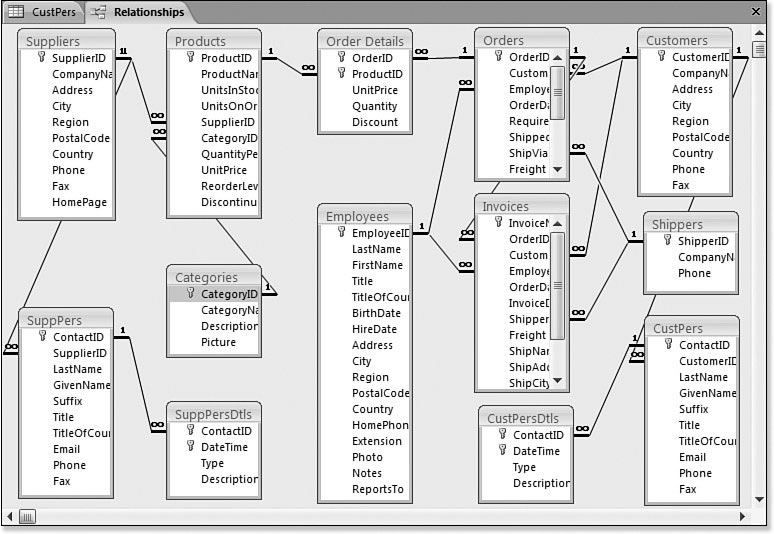
\includegraphics{figures/SampleRetailDatabase.png}

We will cover a few details of data merges that will help you avoid
common and very subtle mistakes that can lead to incorrect inferences.

\hypertarget{set-theory}{%
\section{Set Theory}\label{set-theory}}

In order to merge data \textbf{correctly} you need to understand some
very basic principles of set theory.

\hypertarget{set-theory-functions}{%
\subsection{Set Theory Functions}\label{set-theory-functions}}

Let's assume we have two sets: set1=\emph{{[}A,B{]}},
set2=\emph{{[}B,C{]}}. Each element in this set represents a group of
observations that occurs in the dataset. So B represents people that
occur in both datasets, A represents people that occur only in the first
dataset, and C represents people that only occur in the second dataset.

We can then describe membership through three operations:

\begin{figure}

{\centering 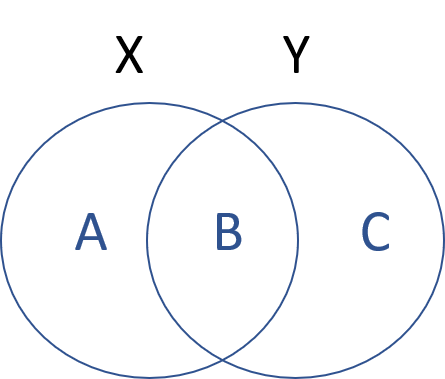
\includegraphics[width=0.7\linewidth]{figures/xy} 

}

\caption{Membership defined by two sets}\label{fig:unnamed-chunk-108}
\end{figure}

\begin{longtable}[]{@{}ll@{}}
\toprule
\begin{minipage}[b]{0.53\columnwidth}\raggedright
Operation\strut
\end{minipage} & \begin{minipage}[b]{0.41\columnwidth}\raggedright
Description\strut
\end{minipage}\tabularnewline
\midrule
\endhead
\begin{minipage}[t]{0.53\columnwidth}\raggedright
union: X\strut
\end{minipage} & \begin{minipage}[t]{0.41\columnwidth}\raggedright
Y\strut
\end{minipage}\tabularnewline
\begin{minipage}[t]{0.53\columnwidth}\raggedright
intersection: X \& Y\strut
\end{minipage} & \begin{minipage}[t]{0.41\columnwidth}\raggedright
The elements shared by both sets: {[}B{]}\strut
\end{minipage}\tabularnewline
\begin{minipage}[t]{0.53\columnwidth}\raggedright
difference: X \& ! Y\strut
\end{minipage} & \begin{minipage}[t]{0.41\columnwidth}\raggedright
The elements in my first set, not in my second {[}A{]} or {[}C{]}\strut
\end{minipage}\tabularnewline
\bottomrule
\end{longtable}

Let's see how this might work in practice with an example of members of
a study:

\begin{Shaded}
\begin{Highlighting}[]
\NormalTok{name <-}\StringTok{ }\KeywordTok{c}\NormalTok{(}\StringTok{"frank"}\NormalTok{,}\StringTok{"wanda"}\NormalTok{,}\StringTok{"sanjay"}\NormalTok{,}\StringTok{"nancy"}\NormalTok{)}
\NormalTok{group <-}\StringTok{ }\KeywordTok{c}\NormalTok{(}\StringTok{"treat"}\NormalTok{,}\StringTok{"treat"}\NormalTok{,}\StringTok{"control"}\NormalTok{,}\StringTok{"control"}\NormalTok{)}
\NormalTok{gender <-}\StringTok{ }\KeywordTok{c}\NormalTok{(}\StringTok{"male"}\NormalTok{,}\StringTok{"female"}\NormalTok{,}\StringTok{"male"}\NormalTok{,}\StringTok{"female"}\NormalTok{)}
\end{Highlighting}
\end{Shaded}

\begin{longtable}[]{@{}ccc@{}}
\toprule
\begin{minipage}[b]{0.11\columnwidth}\centering
name\strut
\end{minipage} & \begin{minipage}[b]{0.13\columnwidth}\centering
group\strut
\end{minipage} & \begin{minipage}[b]{0.13\columnwidth}\centering
gender\strut
\end{minipage}\tabularnewline
\midrule
\endhead
\begin{minipage}[t]{0.11\columnwidth}\centering
frank\strut
\end{minipage} & \begin{minipage}[t]{0.13\columnwidth}\centering
treat\strut
\end{minipage} & \begin{minipage}[t]{0.13\columnwidth}\centering
male\strut
\end{minipage}\tabularnewline
\begin{minipage}[t]{0.11\columnwidth}\centering
wanda\strut
\end{minipage} & \begin{minipage}[t]{0.13\columnwidth}\centering
treat\strut
\end{minipage} & \begin{minipage}[t]{0.13\columnwidth}\centering
female\strut
\end{minipage}\tabularnewline
\begin{minipage}[t]{0.11\columnwidth}\centering
sanjay\strut
\end{minipage} & \begin{minipage}[t]{0.13\columnwidth}\centering
control\strut
\end{minipage} & \begin{minipage}[t]{0.13\columnwidth}\centering
male\strut
\end{minipage}\tabularnewline
\begin{minipage}[t]{0.11\columnwidth}\centering
nancy\strut
\end{minipage} & \begin{minipage}[t]{0.13\columnwidth}\centering
control\strut
\end{minipage} & \begin{minipage}[t]{0.13\columnwidth}\centering
female\strut
\end{minipage}\tabularnewline
\bottomrule
\end{longtable}

For this example let's define set 1 as the treatment group, and set 2 as
all women in the study. Note that set membership is always defined as
binary (you are in the set or out), but it can include multiple criteria
(the set of animals can contains cats, dogs, and mice).

\begin{Shaded}
\begin{Highlighting}[]
\NormalTok{treated <-}\StringTok{ }\NormalTok{name[ group }\OperatorTok{==}\StringTok{ "treat"}\NormalTok{ ]}

\NormalTok{treated }
\CommentTok{### [1] "frank" "wanda"}

\NormalTok{females <-}\StringTok{ }\NormalTok{name[ gender }\OperatorTok{==}\StringTok{ "female"}\NormalTok{ ]}

\NormalTok{females }
\CommentTok{### [1] "wanda" "nancy"}
\end{Highlighting}
\end{Shaded}

Now we can specify group belonging using some convenient set theory
functions: \textbf{union()}, \textbf{setdiff()}, and
\textbf{intersect()}.

\begin{Shaded}
\begin{Highlighting}[]
\KeywordTok{union}\NormalTok{( treated, females )}
\CommentTok{### [1] "frank" "wanda" "nancy"}

\KeywordTok{intersect}\NormalTok{( treated, females )}
\CommentTok{### [1] "wanda"}

\KeywordTok{setdiff}\NormalTok{( treated, females )}
\CommentTok{### [1] "frank"}

\KeywordTok{setdiff}\NormalTok{( females, treated )}
\CommentTok{### [1] "nancy"}
\end{Highlighting}
\end{Shaded}

It is very important to note that \textbf{union()} and
\textbf{intersect()} are symmetric functions, meaning
\emph{intersect(x,y)} will give you the same result as
\emph{intersect(y,x)}. The \textbf{setdiff()} function is not symmetric,
however.

\hypertarget{set-theory-using-logical-operators}{%
\subsection{Set Theory Using Logical
Operators}\label{set-theory-using-logical-operators}}

Typically you will define your groups using logical operators, which
perform the exact same funciton as set theory functions but are a little
more expressive and flexible.

Let's use the same example above where x=``treatment'' and y=``female'',
then consider these cases:

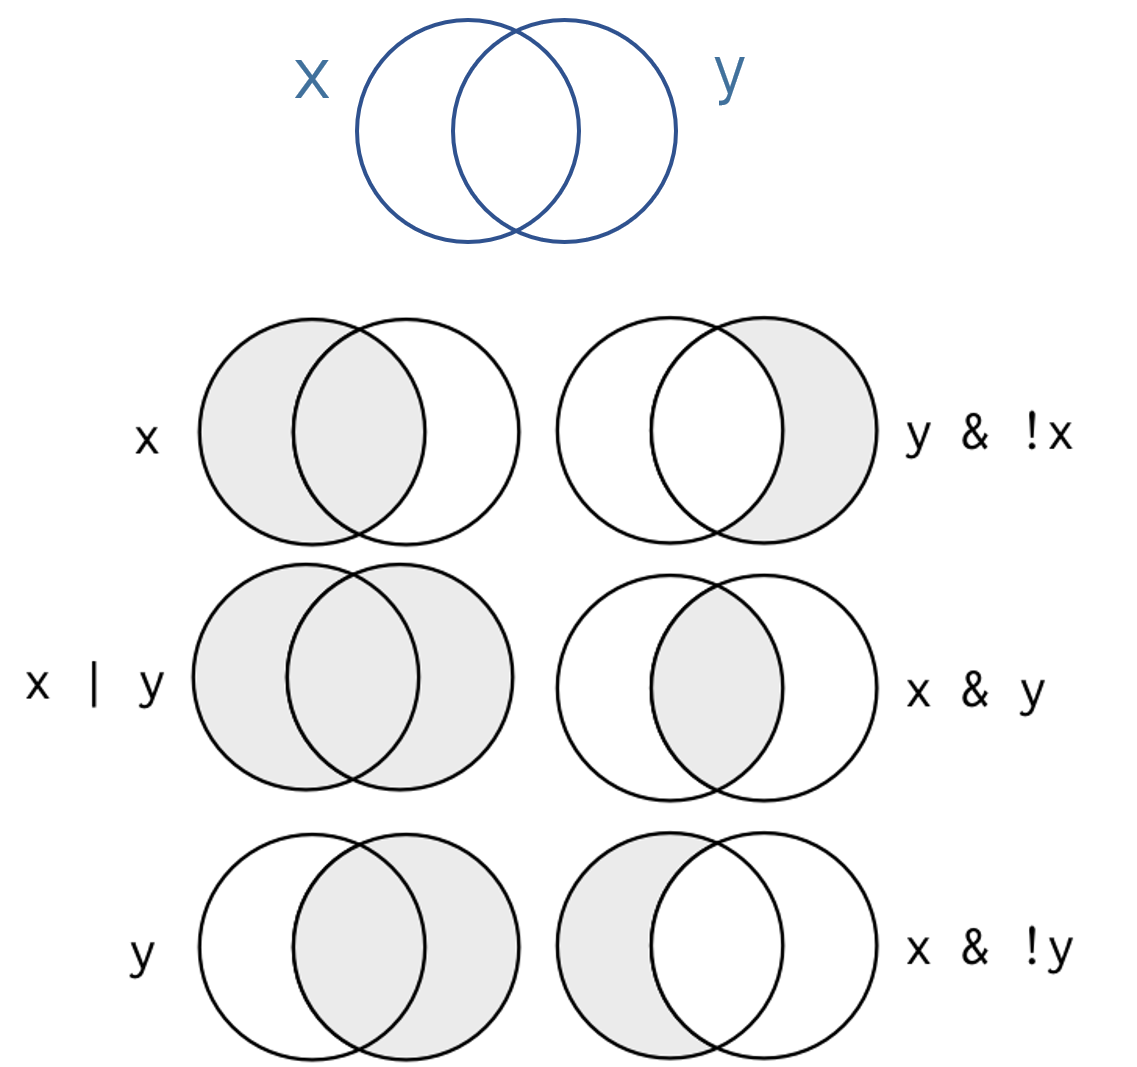
\includegraphics{figures/set_theory.png}

Who belongs in each group?

\begin{longtable}[]{@{}ccc@{}}
\toprule
\begin{minipage}[b]{0.11\columnwidth}\centering
name\strut
\end{minipage} & \begin{minipage}[b]{0.13\columnwidth}\centering
group\strut
\end{minipage} & \begin{minipage}[b]{0.13\columnwidth}\centering
gender\strut
\end{minipage}\tabularnewline
\midrule
\endhead
\begin{minipage}[t]{0.11\columnwidth}\centering
frank\strut
\end{minipage} & \begin{minipage}[t]{0.13\columnwidth}\centering
treat\strut
\end{minipage} & \begin{minipage}[t]{0.13\columnwidth}\centering
male\strut
\end{minipage}\tabularnewline
\begin{minipage}[t]{0.11\columnwidth}\centering
wanda\strut
\end{minipage} & \begin{minipage}[t]{0.13\columnwidth}\centering
treat\strut
\end{minipage} & \begin{minipage}[t]{0.13\columnwidth}\centering
female\strut
\end{minipage}\tabularnewline
\begin{minipage}[t]{0.11\columnwidth}\centering
sanjay\strut
\end{minipage} & \begin{minipage}[t]{0.13\columnwidth}\centering
control\strut
\end{minipage} & \begin{minipage}[t]{0.13\columnwidth}\centering
male\strut
\end{minipage}\tabularnewline
\begin{minipage}[t]{0.11\columnwidth}\centering
nancy\strut
\end{minipage} & \begin{minipage}[t]{0.13\columnwidth}\centering
control\strut
\end{minipage} & \begin{minipage}[t]{0.13\columnwidth}\centering
female\strut
\end{minipage}\tabularnewline
\bottomrule
\end{longtable}

\begin{Shaded}
\begin{Highlighting}[]
\CommentTok{#   x}

\NormalTok{name[ group }\OperatorTok{==}\StringTok{ "treat"}\NormalTok{ ]}
\CommentTok{### [1] "frank" "wanda"}

\CommentTok{#   x & y}

\NormalTok{name[ group }\OperatorTok{==}\StringTok{ "treat"} \OperatorTok{&}\StringTok{ }\NormalTok{gender }\OperatorTok{==}\StringTok{ "female"}\NormalTok{ ]}
\CommentTok{### [1] "wanda"}

\CommentTok{#   x & ! y}

\NormalTok{name[ group }\OperatorTok{==}\StringTok{ "treat"} \OperatorTok{&}\StringTok{ }\NormalTok{gender }\OperatorTok{!=}\StringTok{ "female"}\NormalTok{ ]}
\CommentTok{### [1] "frank"}

\CommentTok{#  x | y}

\NormalTok{name[ group }\OperatorTok{==}\StringTok{ "treat"} \OperatorTok{|}\StringTok{ }\NormalTok{gender }\OperatorTok{==}\StringTok{ "female"}\NormalTok{ ]}
\CommentTok{### [1] "frank" "wanda" "nancy"}
\end{Highlighting}
\end{Shaded}

Who belongs in these groups?

\begin{itemize}
\tightlist
\item
  !x \& !y
\item
  x \& ! ( x \& y )
\item
  ( x \textbar{} y ) \& ! ( x \& y )
\end{itemize}

\hypertarget{merging-data-1}{%
\section{Merging Data}\label{merging-data-1}}

\textbf{The Merge Function}

The merge function joins two datasets. The function requires two
datasets as the arguments, and they need to share a unique ID variable.
Recall the example from above:

\begin{Shaded}
\begin{Highlighting}[]
\KeywordTok{merge}\NormalTok{( customer.info, purchases )}
\CommentTok{###   CUSTOMER.ID FIRST.NAME LAST.NAME       ADDRESS ZIP.CODE PRODUCT PRICE}
\CommentTok{### 1         178     Alvaro    Jaurez  123 Park Ave    57701   video  5.38}
\CommentTok{### 2         178     Alvaro    Jaurez  123 Park Ave    57701  shovel 12.00}
\CommentTok{### 3         269    Latisha     Shane 1600 Penn Ave    20500    book  3.99}
\CommentTok{### 4         269    Latisha     Shane 1600 Penn Ave    20500   purse  8.00}
\CommentTok{### 5         934    Janette   Johnson  456 Candy Ln    57701  mirror  7.64}
\end{Highlighting}
\end{Shaded}

The important thing to keep in mind is that the default merge operation
uses the \textbf{intersection} of the two datasets. It will drop all
elements that don't occur in both datasets. We may want to fine-tune
this as to not lose valuable data and potentially bias our analysis. As
an example, no illegal immigrants will have social security numbers, so
if you are merging using the SSN, you will drop this group from the
data, which could impact your results.

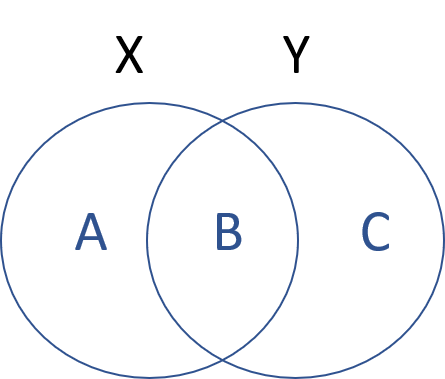
\includegraphics{figures/xy.png}

With a little help from the set theory examples above, we can think
about which portions of the data we wish to drop and which portions we
wish to keep.

\begin{longtable}[]{@{}ll@{}}
\toprule
Argument & Usage\tabularnewline
\midrule
\endhead
all=F & DEFAULT - new dataset contains intersection of X and Y (B
only)\tabularnewline
all=T & New dataset contains union of X and Y (A, B \& C)\tabularnewline
all.x=T & New dataset contains A and B, not C\tabularnewline
all.y=T & New dataset contains B and C, not A\tabularnewline
\bottomrule
\end{longtable}

Here is some demonstrations with examples adapted from the R help file.

\begin{Shaded}
\begin{Highlighting}[]
\NormalTok{authors   }
\CommentTok{###       surname nationality deceased}
\CommentTok{### 1       Tukey          US      yes}
\CommentTok{### 2     Tierney          US       no}
\CommentTok{### 3      Ripley          UK       no}
\CommentTok{### 4      McNeil   Australia       no}
\CommentTok{### 5 Shakespeare     England      yes}

\NormalTok{books    }
\CommentTok{###          name                     title}
\CommentTok{### 1       Tukey Exploratory Data Analysis}
\CommentTok{### 2    Venables Modern Applied Statistics}
\CommentTok{### 3      Ripley        Spatial Statistics}
\CommentTok{### 4      Ripley     Stochastic Simulation}
\CommentTok{### 5      McNeil Interactive Data Analysis}
\CommentTok{### 6 R Core Team      An Introduction to R}


\CommentTok{# adding books to the author bios dataset  ( set B only )}

\KeywordTok{merge}\NormalTok{(authors, books, }\DataTypeTok{by.x =} \StringTok{"surname"}\NormalTok{, }\DataTypeTok{by.y =} \StringTok{"name"}\NormalTok{)    }
\CommentTok{###   surname nationality deceased                     title}
\CommentTok{### 1  McNeil   Australia       no Interactive Data Analysis}
\CommentTok{### 2  Ripley          UK       no        Spatial Statistics}
\CommentTok{### 3  Ripley          UK       no     Stochastic Simulation}
\CommentTok{### 4   Tukey          US      yes Exploratory Data Analysis}



\CommentTok{# adding author bios to the books dataset  ( set B only )}

\KeywordTok{merge}\NormalTok{(books, authors, }\DataTypeTok{by.x =} \StringTok{"name"}\NormalTok{, }\DataTypeTok{by.y =} \StringTok{"surname"}\NormalTok{)    }
\CommentTok{###     name                     title nationality deceased}
\CommentTok{### 1 McNeil Interactive Data Analysis   Australia       no}
\CommentTok{### 2 Ripley        Spatial Statistics          UK       no}
\CommentTok{### 3 Ripley     Stochastic Simulation          UK       no}
\CommentTok{### 4  Tukey Exploratory Data Analysis          US      yes}



\CommentTok{# keep books without author bios, lose authors without books  ( sets A and B )}

\KeywordTok{merge}\NormalTok{( books, authors, }\DataTypeTok{by.x =} \StringTok{"name"}\NormalTok{, }\DataTypeTok{by.y =} \StringTok{"surname"}\NormalTok{, }\DataTypeTok{all.x=}\NormalTok{T )     }
\CommentTok{###          name                     title nationality deceased}
\CommentTok{### 1      McNeil Interactive Data Analysis   Australia       no}
\CommentTok{### 2 R Core Team      An Introduction to R        <NA>     <NA>}
\CommentTok{### 3      Ripley        Spatial Statistics          UK       no}
\CommentTok{### 4      Ripley     Stochastic Simulation          UK       no}
\CommentTok{### 5       Tukey Exploratory Data Analysis          US      yes}
\CommentTok{### 6    Venables Modern Applied Statistics        <NA>     <NA>}



\CommentTok{# keep authors without book listed, lose books without author bios   ( sets B and C )}

\KeywordTok{merge}\NormalTok{( books, authors, }\DataTypeTok{by.x =} \StringTok{"name"}\NormalTok{, }\DataTypeTok{by.y =} \StringTok{"surname"}\NormalTok{, }\DataTypeTok{all.y=}\NormalTok{T )    }
\CommentTok{###          name                     title nationality deceased}
\CommentTok{### 1      McNeil Interactive Data Analysis   Australia       no}
\CommentTok{### 2      Ripley        Spatial Statistics          UK       no}
\CommentTok{### 3      Ripley     Stochastic Simulation          UK       no}
\CommentTok{### 4 Shakespeare                      <NA>     England      yes}
\CommentTok{### 5     Tierney                      <NA>          US       no}
\CommentTok{### 6       Tukey Exploratory Data Analysis          US      yes}



\CommentTok{# dont' throw out any data   ( sets A and B and C )}

\KeywordTok{merge}\NormalTok{( books, authors, }\DataTypeTok{by.x =} \StringTok{"name"}\NormalTok{, }\DataTypeTok{by.y =} \StringTok{"surname"}\NormalTok{, }\DataTypeTok{all=}\NormalTok{T )   }
\CommentTok{###          name                     title nationality deceased}
\CommentTok{### 1      McNeil Interactive Data Analysis   Australia       no}
\CommentTok{### 2 R Core Team      An Introduction to R        <NA>     <NA>}
\CommentTok{### 3      Ripley        Spatial Statistics          UK       no}
\CommentTok{### 4      Ripley     Stochastic Simulation          UK       no}
\CommentTok{### 5 Shakespeare                      <NA>     England      yes}
\CommentTok{### 6     Tierney                      <NA>          US       no}
\CommentTok{### 7       Tukey Exploratory Data Analysis          US      yes}
\CommentTok{### 8    Venables Modern Applied Statistics        <NA>     <NA>}
\end{Highlighting}
\end{Shaded}

Also note that the order of your datasets in the argument list will
impact the inclusion or exclusion of elements.

merge( x, y, all=F ) EQUALS merge( y, x, all=F )

merge( x, y, all.x=T ) DOES NOT EQUAL merge( y, x, all.x=T )

\hypertarget{the-by.x-and-by.y-arguments}{%
\subsection{The by.x and by.y
Arguments}\label{the-by.x-and-by.y-arguments}}

When you use the default \textbf{merge()} function without specifying
the variables to merge upon, the function will check for common variable
names across the two datasets. If there are multiple, it will join the
shared variables to create a new unique key. This might be problematic
if that was not the intent.

Take the example of combining fielding and salary data in the Lahman
package. If we are not explicit about the merge variable, we may get odd
results. Note that they two datasets share four ID variables.

\begin{Shaded}
\begin{Highlighting}[]
\KeywordTok{library}\NormalTok{( Lahman )}
\KeywordTok{data}\NormalTok{( Fielding )}
\KeywordTok{data}\NormalTok{( Salaries )}
\end{Highlighting}
\end{Shaded}

\begin{Shaded}
\begin{Highlighting}[]
\KeywordTok{intersect}\NormalTok{( }\KeywordTok{names}\NormalTok{(Fielding), }\KeywordTok{names}\NormalTok{(Salaries) )}
\CommentTok{### [1] "playerID" "yearID"   "teamID"   "lgID"}

\CommentTok{# merge id}

\NormalTok{int <-}\StringTok{ }\KeywordTok{intersect}\NormalTok{( }\KeywordTok{names}\NormalTok{(Fielding), }\KeywordTok{names}\NormalTok{(Salaries) )}

\KeywordTok{paste}\NormalTok{( int[}\DecValTok{1}\NormalTok{],int[}\DecValTok{2}\NormalTok{],int[}\DecValTok{3}\NormalTok{],int[}\DecValTok{4}\NormalTok{], }\DataTypeTok{sep=}\StringTok{"."}\NormalTok{ )}
\CommentTok{### [1] "playerID.yearID.teamID.lgID"}
\end{Highlighting}
\end{Shaded}

To avoid problems, be explicit using the \emph{by.x} and \emph{by.x}
arguments to control which variable is used for the merge.

\begin{Shaded}
\begin{Highlighting}[]
\KeywordTok{head}\NormalTok{( }\KeywordTok{merge}\NormalTok{( Salaries, Fielding ) )}
\CommentTok{###   yearID teamID lgID  playerID salary stint POS  G GS InnOuts  PO  A E DP}
\CommentTok{### 1   1985    ATL   NL barkele01 870000     1   P 20 18     221   2  9 1  0}
\CommentTok{### 2   1985    ATL   NL bedrost01 550000     1   P 37 37     620  13 23 4  3}
\CommentTok{### 3   1985    ATL   NL benedbr01 545000     1   C 70 67    1698 314 35 4  1}
\CommentTok{### 4   1985    ATL   NL  campri01 633333     1   P 66  2     383   7 13 4  3}
\CommentTok{### 5   1985    ATL   NL ceronri01 625000     1   C 91 76    2097 384 48 6  4}
\CommentTok{### 6   1985    ATL   NL chambch01 800000     1  1B 39 27     814 299 25 1 31}
\CommentTok{###   PB WP SB CS ZR}
\CommentTok{### 1 NA NA NA NA NA}
\CommentTok{### 2 NA NA NA NA NA}
\CommentTok{### 3  1  9 65 24  1}
\CommentTok{### 4 NA NA NA NA NA}
\CommentTok{### 5  6 20 69 29  1}
\CommentTok{### 6 NA NA NA NA NA}
\KeywordTok{head}\NormalTok{( }\KeywordTok{merge}\NormalTok{( Salaries, Fielding, }\DataTypeTok{by.x=}\StringTok{"playerID"}\NormalTok{, }\DataTypeTok{by.y=}\StringTok{"playerID"}\NormalTok{ ) )}
\CommentTok{###    playerID yearID.x teamID.x lgID.x  salary yearID.y stint teamID.y}
\CommentTok{### 1 aardsda01     2010      SEA     AL 2750000     2009     1      SEA}
\CommentTok{### 2 aardsda01     2010      SEA     AL 2750000     2015     1      ATL}
\CommentTok{### 3 aardsda01     2010      SEA     AL 2750000     2006     1      CHN}
\CommentTok{### 4 aardsda01     2010      SEA     AL 2750000     2008     1      BOS}
\CommentTok{### 5 aardsda01     2010      SEA     AL 2750000     2013     1      NYN}
\CommentTok{### 6 aardsda01     2010      SEA     AL 2750000     2012     1      NYA}
\CommentTok{###   lgID.y POS  G GS InnOuts PO A E DP PB WP SB CS ZR}
\CommentTok{### 1     AL   P 73  0     214  2 5 0  1 NA NA NA NA NA}
\CommentTok{### 2     NL   P 33  0      92  0 1 1  0 NA NA NA NA NA}
\CommentTok{### 3     NL   P 45  0     159  1 5 0  1 NA NA NA NA NA}
\CommentTok{### 4     AL   P 47  0     146  3 6 0  0 NA NA NA NA NA}
\CommentTok{### 5     NL   P 43  0     119  1 5 0  0 NA NA NA NA NA}
\CommentTok{### 6     AL   P  1  0       3  0 0 0  0 NA NA NA NA NA}
\end{Highlighting}
\end{Shaded}

\hypertarget{non-unique-observations-in-id-variables}{%
\section{Non-Unique Observations in ID
Variables}\label{non-unique-observations-in-id-variables}}

In some rare instances, you will need to merge to datasets that have
non-singular elements in the unique key ID variables, meaning each
observation / individual appears more than one time in the data. Note
that in this case, for each occurance of an observation / individual in
your X dataset, you will merge once with each occurance of the same
observation / individual in the Y dataset. The result will be a
multiplicative expansion of the size of your dataset.

For example, if John appears on four separate rows of X, and three
seperate rows of Y, the new dataset will contain 12 rows of John (4 x 3
= 12).

dataset X contains four separate instances of an individual {[} X1, X2,
X3, X4 {]}

dataset Y contains three separate instances of an individual {[} Y1, Y2,
Y3 {]}

After the merge we have one row for each pair:

X1-Y1\\
X1-Y2\\
X1-Y3\\
X2-Y1\\
X2-Y2\\
X2-Y3\\
X3-Y1\\
X3-Y2\\
X3-Y3\\
X4-Y1\\
X4-Y2\\
X4-Y3

For example, perhaps a sales company has a database that keeps track of
biographical data, and sales performance. Perhaps we want to see if
there is peak age for sales performance. We need to merge these
datasets.

\begin{Shaded}
\begin{Highlighting}[]
\NormalTok{bio <-}\StringTok{ }\KeywordTok{data.frame}\NormalTok{( }\DataTypeTok{name=}\KeywordTok{c}\NormalTok{(}\StringTok{"John"}\NormalTok{,}\StringTok{"John"}\NormalTok{,}\StringTok{"John"}\NormalTok{),}
                   \DataTypeTok{year=}\KeywordTok{c}\NormalTok{(}\DecValTok{2000}\NormalTok{,}\DecValTok{2001}\NormalTok{,}\DecValTok{2002}\NormalTok{),}
                   \DataTypeTok{age=}\KeywordTok{c}\NormalTok{(}\DecValTok{43}\NormalTok{,}\DecValTok{44}\NormalTok{,}\DecValTok{45}\NormalTok{) )}

\NormalTok{performance <-}\StringTok{ }\KeywordTok{data.frame}\NormalTok{( }\DataTypeTok{name=}\KeywordTok{c}\NormalTok{(}\StringTok{"John"}\NormalTok{,}\StringTok{"John"}\NormalTok{,}\StringTok{"John"}\NormalTok{),}
                           \DataTypeTok{year=}\KeywordTok{c}\NormalTok{(}\DecValTok{2000}\NormalTok{,}\DecValTok{2001}\NormalTok{,}\DecValTok{2002}\NormalTok{),}
                           \DataTypeTok{sales=}\KeywordTok{c}\NormalTok{(}\StringTok{"15k"}\NormalTok{,}\StringTok{"20k"}\NormalTok{,}\StringTok{"17k"}\NormalTok{) )}

\CommentTok{# correct merge}

\KeywordTok{merge}\NormalTok{( bio, performance, }\DataTypeTok{by.x=}\KeywordTok{c}\NormalTok{(}\StringTok{"name"}\NormalTok{,}\StringTok{"year"}\NormalTok{), }\DataTypeTok{by.y=}\KeywordTok{c}\NormalTok{(}\StringTok{"name"}\NormalTok{,}\StringTok{"year"}\NormalTok{) ) }
\CommentTok{###   name year age sales}
\CommentTok{### 1 John 2000  43   15k}
\CommentTok{### 2 John 2001  44   20k}
\CommentTok{### 3 John 2002  45   17k}


\CommentTok{# incorrect merge}

\KeywordTok{merge}\NormalTok{( bio, performance, }\DataTypeTok{by.x=}\KeywordTok{c}\NormalTok{(}\StringTok{"name"}\NormalTok{), }\DataTypeTok{by.y=}\KeywordTok{c}\NormalTok{(}\StringTok{"name"}\NormalTok{) )  }
\CommentTok{###   name year.x age year.y sales}
\CommentTok{### 1 John   2000  43   2000   15k}
\CommentTok{### 2 John   2000  43   2001   20k}
\CommentTok{### 3 John   2000  43   2002   17k}
\CommentTok{### 4 John   2001  44   2000   15k}
\CommentTok{### 5 John   2001  44   2001   20k}
\CommentTok{### 6 John   2001  44   2002   17k}
\CommentTok{### 7 John   2002  45   2000   15k}
\CommentTok{### 8 John   2002  45   2001   20k}
\CommentTok{### 9 John   2002  45   2002   17k}
\end{Highlighting}
\end{Shaded}

\textbf{It is good practice to check the size (number of rows) of your
dataset before and after a merge. If it has expanded, chances are you
either used the wrong unique IDs, or your dataset contains duplicates.}

\hypertarget{example-of-incorrect-merge}{%
\subsection{Example of Incorrect
Merge}\label{example-of-incorrect-merge}}

Here is a tangible example using the Lahman baseball dataset. Perhaps we
want to examine the relationship between fielding position and salary.
The \emph{Fielding} dataset contains fielding position information, and
the \emph{Salaries} dataset contains salary information. We can merge
these two datasets using the \emph{playerID} field.

If we are not thoughtful about this, however, we will end up causing
problems. Let's look at an example using Kirby Pucket.

\begin{Shaded}
\begin{Highlighting}[]
\NormalTok{kirby.fielding <-}\StringTok{ }\NormalTok{Fielding[ Fielding}\OperatorTok{$}\NormalTok{playerID }\OperatorTok{==}\StringTok{ "puckeki01"}\NormalTok{ , ]}

\KeywordTok{head}\NormalTok{( kirby.fielding )}
\CommentTok{###        playerID yearID stint teamID lgID POS   G  GS InnOuts  PO  A E DP}
\CommentTok{### 83848 puckeki01   1984     1    MIN   AL  OF 128 128    3377 438 16 3  4}
\CommentTok{### 85157 puckeki01   1985     1    MIN   AL  OF 161 160    4213 465 19 8  5}
\CommentTok{### 86489 puckeki01   1986     1    MIN   AL  OF 160 157    4155 429  8 6  3}
\CommentTok{### 87896 puckeki01   1987     1    MIN   AL  OF 147 147    3820 341  8 5  2}
\CommentTok{### 89264 puckeki01   1988     1    MIN   AL  OF 158 157    4049 450 12 3  4}
\CommentTok{### 90685 puckeki01   1989     1    MIN   AL  OF 157 154    3985 438 13 4  3}
\CommentTok{###       PB WP SB CS ZR}
\CommentTok{### 83848 NA NA NA NA NA}
\CommentTok{### 85157 NA NA NA NA NA}
\CommentTok{### 86489 NA NA NA NA NA}
\CommentTok{### 87896 NA NA NA NA NA}
\CommentTok{### 89264 NA NA NA NA NA}
\CommentTok{### 90685 NA NA NA NA NA}

\KeywordTok{nrow}\NormalTok{( kirby.fielding )}
\CommentTok{### [1] 21}

\NormalTok{kirby.salary <-}\StringTok{ }\NormalTok{Salaries[ Salaries}\OperatorTok{$}\NormalTok{playerID }\OperatorTok{==}\StringTok{ "puckeki01"}\NormalTok{ , ]}

\KeywordTok{head}\NormalTok{( kirby.salary )}
\CommentTok{###      yearID teamID lgID  playerID  salary}
\CommentTok{### 280    1985    MIN   AL puckeki01  130000}
\CommentTok{### 917    1986    MIN   AL puckeki01  255000}
\CommentTok{### 1610   1987    MIN   AL puckeki01  465000}
\CommentTok{### 2244   1988    MIN   AL puckeki01 1090000}
\CommentTok{### 2922   1989    MIN   AL puckeki01 2000000}
\CommentTok{### 3717   1990    MIN   AL puckeki01 2816667}

\KeywordTok{nrow}\NormalTok{( kirby.salary )}
\CommentTok{### [1] 13}

\NormalTok{kirby.field.salary <-}\StringTok{ }\KeywordTok{merge}\NormalTok{( kirby.fielding, kirby.salary, }\DataTypeTok{by.x=}\StringTok{"playerID"}\NormalTok{, }\DataTypeTok{by.y=}\StringTok{"playerID"}\NormalTok{ )}

\KeywordTok{head}\NormalTok{( }\KeywordTok{select}\NormalTok{( kirby.field.salary, yearID.x, yearID.y,   POS,    G,  GS, salary ) )}
\CommentTok{###   yearID.x yearID.y POS   G  GS  salary}
\CommentTok{### 1     1984     1985  OF 128 128  130000}
\CommentTok{### 2     1984     1986  OF 128 128  255000}
\CommentTok{### 3     1984     1987  OF 128 128  465000}
\CommentTok{### 4     1984     1988  OF 128 128 1090000}
\CommentTok{### 5     1984     1989  OF 128 128 2000000}
\CommentTok{### 6     1984     1990  OF 128 128 2816667}

\KeywordTok{nrow}\NormalTok{( kirby.field.salary )}
\CommentTok{### [1] 273}

\DecValTok{21}\OperatorTok{*}\DecValTok{13}
\CommentTok{### [1] 273}
\end{Highlighting}
\end{Shaded}

What we have done here is taken each year of fielding data, and matched
it to \textbf{every} year of salary data. We can see that we have 21
fielding observations and 13 years of salary data, so our resulting
dataset is 273 observation pairs.

This merge also makes it difficult to answer the question of the
relationship between fielding position and salary if players change
positions over time.

The correct merge in this case would be a merge on a playerID-yearID
pair. We can create a unique key by combining playerID and yearID using
\textbf{paste()}:

\begin{Shaded}
\begin{Highlighting}[]

\KeywordTok{head}\NormalTok{( }\KeywordTok{paste}\NormalTok{( kirby.fielding}\OperatorTok{$}\NormalTok{playerID, kirby.fielding}\OperatorTok{$}\NormalTok{yearID, }\DataTypeTok{sep=}\StringTok{"."}\NormalTok{) )}
\CommentTok{### [1] "puckeki01.1984" "puckeki01.1985" "puckeki01.1986" "puckeki01.1987"}
\CommentTok{### [5] "puckeki01.1988" "puckeki01.1989"}
\end{Highlighting}
\end{Shaded}

But there is a simple solution as the merge function also allows for
multiple variables to be used for a \textbf{merge()} command.

\begin{Shaded}
\begin{Highlighting}[]
\NormalTok{kirby.field.salary <-}\StringTok{ }\KeywordTok{merge}\NormalTok{( kirby.fielding, kirby.salary, }
                            \DataTypeTok{by.x=}\KeywordTok{c}\NormalTok{(}\StringTok{"playerID"}\NormalTok{,}\StringTok{"yearID"}\NormalTok{), }
                            \DataTypeTok{by.y=}\KeywordTok{c}\NormalTok{(}\StringTok{"playerID"}\NormalTok{,}\StringTok{"yearID"}\NormalTok{)   )}

\KeywordTok{nrow}\NormalTok{( kirby.field.salary )}
\CommentTok{### [1] 20}
\end{Highlighting}
\end{Shaded}

\hypertarget{the-in-function}{%
\section{The \%in\% function}\label{the-in-function}}

Since we are talking about intersections and matches, I want to briefly
introduce the \textbf{\%in\%} function. It is a combination of the two.

The \textbf{intersect()} function returns a list of unique matches
between two vectors.

\begin{Shaded}
\begin{Highlighting}[]
\KeywordTok{data}\NormalTok{(Salaries)}
\KeywordTok{data}\NormalTok{(Fielding)}
\KeywordTok{intersect}\NormalTok{( }\KeywordTok{names}\NormalTok{(Salaries), }\KeywordTok{names}\NormalTok{(Fielding) )}
\CommentTok{### [1] "yearID"   "teamID"   "lgID"     "playerID"}
\end{Highlighting}
\end{Shaded}

The \textbf{match()} function returns the position of matched elements.

\begin{Shaded}
\begin{Highlighting}[]
\NormalTok{x <-}\StringTok{ }\KeywordTok{c}\NormalTok{(}\StringTok{"A"}\NormalTok{,}\StringTok{"B"}\NormalTok{,}\StringTok{"C"}\NormalTok{,}\StringTok{"B"}\NormalTok{)}

\NormalTok{y <-}\StringTok{ }\KeywordTok{c}\NormalTok{(}\StringTok{"B"}\NormalTok{,}\StringTok{"D"}\NormalTok{,}\StringTok{"A"}\NormalTok{,}\StringTok{"F"}\NormalTok{)}

\KeywordTok{match}\NormalTok{( x, y )}
\CommentTok{### [1]  3  1 NA  1}
\end{Highlighting}
\end{Shaded}

The \textbf{\%in\%} function returns a logical vector, where TRUE
signifies that the element in \emph{y} also occurs in \emph{x}. In other
words, does a specific element in \emph{y} belong to the intersection of
\emph{x},\emph{y}.

This is very useful for creating subsets of data that belong to both
sets.

\begin{Shaded}
\begin{Highlighting}[]
\NormalTok{x <-}\StringTok{ }\KeywordTok{c}\NormalTok{(}\StringTok{"A"}\NormalTok{,}\StringTok{"B"}\NormalTok{,}\StringTok{"C"}\NormalTok{)}

\NormalTok{y <-}\StringTok{ }\KeywordTok{c}\NormalTok{(}\StringTok{"B"}\NormalTok{,}\StringTok{"D"}\NormalTok{,}\StringTok{"A"}\NormalTok{,}\StringTok{"B"}\NormalTok{,}\StringTok{"F"}\NormalTok{,}\StringTok{"B"}\NormalTok{)}

\NormalTok{y }\OperatorTok\StringTok{ }\NormalTok{x }\CommentTok{# does each element of y occur anywhere in x?}
\CommentTok{### [1]  TRUE FALSE  TRUE  TRUE FALSE  TRUE}

\NormalTok{y[ y }\OperatorTok\StringTok{ }\NormalTok{x] }\CommentTok{# keep only data that occurs in both}
\CommentTok{### [1] "B" "A" "B" "B"}
\end{Highlighting}
\end{Shaded}

\hypertarget{the-match-function}{%
\section{The Match Function}\label{the-match-function}}

Often times we do not need to merge data, we may just need sort data in
one dataset so that it matches the order of another dataset. This is
accomplished using the \textbf{match()} function.

Note that we can rearrange the order of a dataset by referencing the
desired position.

\begin{Shaded}
\begin{Highlighting}[]

\NormalTok{x <-}\StringTok{ }\KeywordTok{c}\NormalTok{(}\StringTok{"Second"}\NormalTok{,}\StringTok{"Third"}\NormalTok{,}\StringTok{"First"}\NormalTok{)}

\NormalTok{x}
\CommentTok{### [1] "Second" "Third"  "First"}

\NormalTok{x[ }\KeywordTok{c}\NormalTok{(}\DecValTok{3}\NormalTok{,}\DecValTok{1}\NormalTok{,}\DecValTok{2}\NormalTok{) ]}
\CommentTok{### [1] "First"  "Second" "Third"}
\end{Highlighting}
\end{Shaded}

The \textbf{match()} function returns the \emph{positions} of matches of
its \emph{first} vector to the \emph{second} vector listed in the
arguments. Or in other words, the \emph{order} that vector 2 would need
to follow to match vector 1.

\begin{Shaded}
\begin{Highlighting}[]

\NormalTok{x <-}\StringTok{ }\KeywordTok{c}\NormalTok{(}\StringTok{"A"}\NormalTok{,}\StringTok{"B"}\NormalTok{,}\StringTok{"C"}\NormalTok{)}

\NormalTok{y <-}\StringTok{ }\KeywordTok{c}\NormalTok{(}\StringTok{"B"}\NormalTok{,}\StringTok{"D"}\NormalTok{,}\StringTok{"A"}\NormalTok{)}

\KeywordTok{cbind}\NormalTok{( x, y )}
\CommentTok{###      x   y  }
\CommentTok{### [1,] "A" "B"}
\CommentTok{### [2,] "B" "D"}
\CommentTok{### [3,] "C" "A"}

\KeywordTok{match}\NormalTok{( x, y )}
\CommentTok{### [1]  3  1 NA}

\KeywordTok{match}\NormalTok{( y, x) }\CommentTok{# not a symmetric operation!}
\CommentTok{### [1]  2 NA  1}

\CommentTok{# In the y vector:}
\CommentTok{#}
\CommentTok{#  [3]=A}
\CommentTok{#  [1]=B}
\CommentTok{# [NA]=D (no match)}

\NormalTok{order.y <-}\StringTok{ }\KeywordTok{match}\NormalTok{( x, y )}

\NormalTok{y[ order.y ]}
\CommentTok{### [1] "A" "B" NA}
\end{Highlighting}
\end{Shaded}

We can see that \textbf{match()} returns the correct order to put
\emph{y} in so that it matches the order of \emph{x}. In the re-ordered
vector, the first element is the original third element \emph{A}, the
second element is the original first element \emph{B}, and there is no
third element because \emph{D} did not match anything in \emph{x}.

Note the order of arguments in the function:

\begin{quote}
match( data I want to match to , data I need to re-order )
\end{quote}

We can use this position information to re-order \emph{y} as follows:

\begin{Shaded}
\begin{Highlighting}[]

\NormalTok{x <-}\StringTok{ }\KeywordTok{sample}\NormalTok{( LETTERS[}\DecValTok{1}\OperatorTok{:}\DecValTok{15}\NormalTok{], }\DataTypeTok{size=}\DecValTok{10}\NormalTok{ )}

\NormalTok{y <-}\StringTok{ }\KeywordTok{sample}\NormalTok{( LETTERS[}\DecValTok{1}\OperatorTok{:}\DecValTok{15}\NormalTok{], }\DataTypeTok{size=}\DecValTok{10}\NormalTok{ )}

\KeywordTok{cbind}\NormalTok{( x, y )}
\CommentTok{###       x   y  }
\CommentTok{###  [1,] "C" "G"}
\CommentTok{###  [2,] "K" "A"}
\CommentTok{###  [3,] "E" "E"}
\CommentTok{###  [4,] "A" "F"}
\CommentTok{###  [5,] "N" "I"}
\CommentTok{###  [6,] "O" "H"}
\CommentTok{###  [7,] "M" "B"}
\CommentTok{###  [8,] "F" "N"}
\CommentTok{###  [9,] "B" "L"}
\CommentTok{### [10,] "G" "C"}

\NormalTok{order.y <-}\StringTok{ }\KeywordTok{match}\NormalTok{( x, y )}

\NormalTok{y.new <-}\StringTok{ }\NormalTok{y[ order.y ]}

\KeywordTok{cbind}\NormalTok{( x, y.new )}
\CommentTok{###       x   y.new}
\CommentTok{###  [1,] "C" "C"  }
\CommentTok{###  [2,] "K" NA   }
\CommentTok{###  [3,] "E" "E"  }
\CommentTok{###  [4,] "A" "A"  }
\CommentTok{###  [5,] "N" "N"  }
\CommentTok{###  [6,] "O" NA   }
\CommentTok{###  [7,] "M" NA   }
\CommentTok{###  [8,] "F" "F"  }
\CommentTok{###  [9,] "B" "B"  }
\CommentTok{### [10,] "G" "G"}


\CommentTok{# Note the result if you confuse the order or arguments}

\NormalTok{order.y <-}\StringTok{ }\KeywordTok{match}\NormalTok{( y, x )}

\NormalTok{y.new <-}\StringTok{ }\NormalTok{y[ order.y ]}

\KeywordTok{cbind}\NormalTok{( x, y.new )}
\CommentTok{###       x   y.new}
\CommentTok{###  [1,] "C" "C"  }
\CommentTok{###  [2,] "K" "F"  }
\CommentTok{###  [3,] "E" "E"  }
\CommentTok{###  [4,] "A" "N"  }
\CommentTok{###  [5,] "N" NA   }
\CommentTok{###  [6,] "O" NA   }
\CommentTok{###  [7,] "M" "L"  }
\CommentTok{###  [8,] "F" "I"  }
\CommentTok{###  [9,] "B" NA   }
\CommentTok{### [10,] "G" "G"}
\end{Highlighting}
\end{Shaded}

This comes in handy when we are matching information between two tables.
For example, in GIS the map regions follow a specific order but your
data does not. Create a color scheme for levels of your data, and then
re-order the colors so they match the correct region on the map. In this
example, we will look at unemployment levels by county.

\begin{Shaded}
\begin{Highlighting}[]

\KeywordTok{library}\NormalTok{( maps )}
\KeywordTok{data}\NormalTok{( county.fips )}
\KeywordTok{data}\NormalTok{( unemp )}

\KeywordTok{map}\NormalTok{( }\DataTypeTok{database=}\StringTok{"county"}\NormalTok{ )}

\CommentTok{# assign a color to each level of unemployment, red = high, gray = medium, blue = low}

\NormalTok{color.function <-}\StringTok{ }\KeywordTok{colorRampPalette}\NormalTok{( }\KeywordTok{c}\NormalTok{(}\StringTok{"steelblue"}\NormalTok{, }\StringTok{"gray70"}\NormalTok{, }\StringTok{"firebrick"}\NormalTok{) )}


\NormalTok{color.vector <-}\StringTok{ }\KeywordTok{cut}\NormalTok{( }\KeywordTok{rank}\NormalTok{(unemp}\OperatorTok{$}\NormalTok{unemp), }\DataTypeTok{breaks=}\DecValTok{7}\NormalTok{, }\DataTypeTok{labels=}\KeywordTok{color.function}\NormalTok{( }\DecValTok{7}\NormalTok{ ) )}

\NormalTok{color.vector <-}\StringTok{ }\KeywordTok{as.character}\NormalTok{( color.vector )}

\KeywordTok{head}\NormalTok{( color.vector )}
\CommentTok{### [1] "#B28282" "#B28282" "#B22222" "#B25252" "#B28282" "#B22222"}

\CommentTok{# doesn't look quite right}

\KeywordTok{map}\NormalTok{( }\DataTypeTok{database=}\StringTok{"county"}\NormalTok{, }\DataTypeTok{col=}\NormalTok{color.vector, }\DataTypeTok{fill=}\NormalTok{T, }\DataTypeTok{lty=}\DecValTok{0}\NormalTok{ )}


\CommentTok{# what went wrong here? }

\CommentTok{# our unemployment data (and thus the color vector) follows a different order}

\KeywordTok{cbind}\NormalTok{( }\DataTypeTok{map.id=}\NormalTok{county.fips}\OperatorTok{$}\NormalTok{fips, }\DataTypeTok{data.id=}\NormalTok{unemp}\OperatorTok{$}\NormalTok{fips, color.vector )[ }\DecValTok{2500}\OperatorTok{:}\DecValTok{2510}\NormalTok{ , ]}
\CommentTok{###       map.id  data.id color.vector}
\CommentTok{###  [1,] "48011" "47149" "#B28282"   }
\CommentTok{###  [2,] "48013" "47151" "#B22222"   }
\CommentTok{###  [3,] "48015" "47153" "#B22222"   }
\CommentTok{###  [4,] "48017" "47155" "#B28282"   }
\CommentTok{###  [5,] "48019" "47157" "#B28282"   }
\CommentTok{###  [6,] "48021" "47159" "#B22222"   }
\CommentTok{###  [7,] "48023" "47161" "#B25252"   }
\CommentTok{###  [8,] "48025" "47163" "#B3B3B3"   }
\CommentTok{###  [9,] "48027" "47165" "#B28282"   }
\CommentTok{### [10,] "48029" "47167" "#B25252"   }
\CommentTok{### [11,] "48031" "47169" "#B25252"}

\CommentTok{# place the color vector in the correct order}

\NormalTok{this.order <-}\StringTok{ }\KeywordTok{match}\NormalTok{( county.fips}\OperatorTok{$}\NormalTok{fips, unemp}\OperatorTok{$}\NormalTok{fips )}

\NormalTok{color.vec.ordered <-}\StringTok{ }\NormalTok{color.vector[ this.order ]}

\CommentTok{# colors now match their correct counties}

\KeywordTok{map}\NormalTok{( }\DataTypeTok{database=}\StringTok{"county"}\NormalTok{, }\DataTypeTok{col=}\NormalTok{color.vec.ordered, }\DataTypeTok{fill=}\NormalTok{T, }\DataTypeTok{lty=}\DecValTok{0}\NormalTok{ )}
\KeywordTok{title}\NormalTok{( }\DataTypeTok{main=}\StringTok{"Unemployment Levels by County in 2009"}\NormalTok{)}
\end{Highlighting}
\end{Shaded}

\begin{center}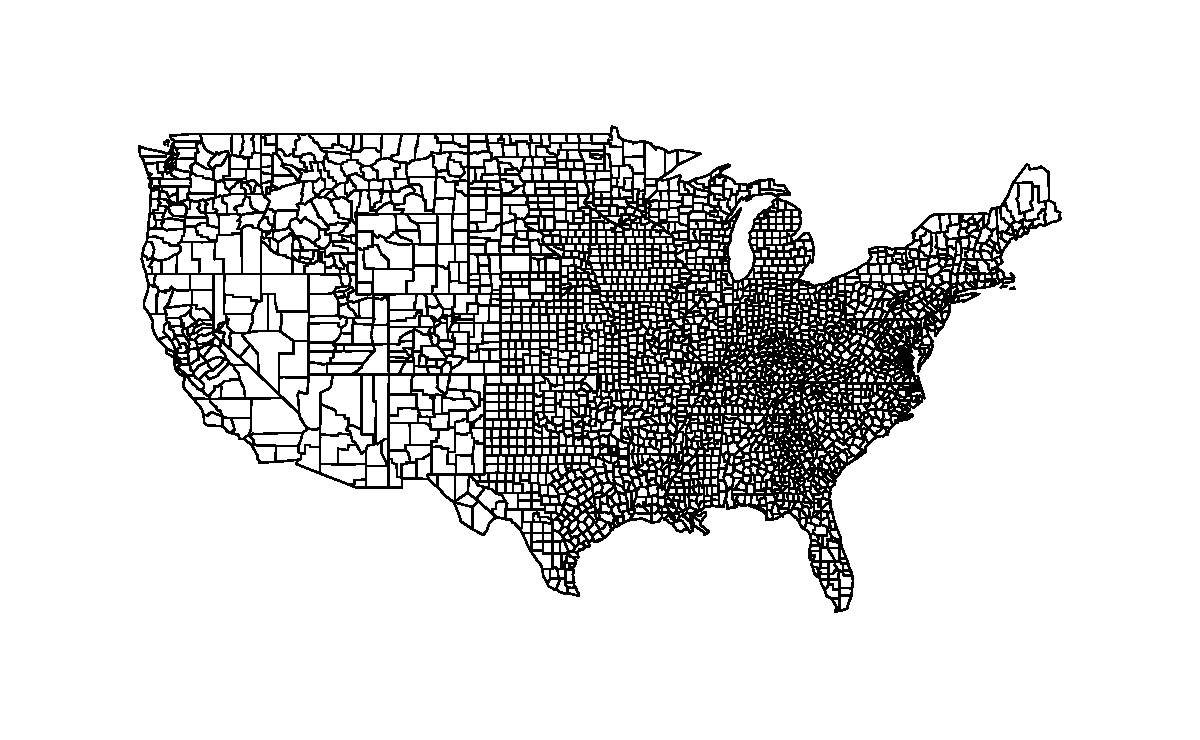
\includegraphics[width=0.7\linewidth]{DS4PS-I_files/figure-latex/unnamed-chunk-131-1} 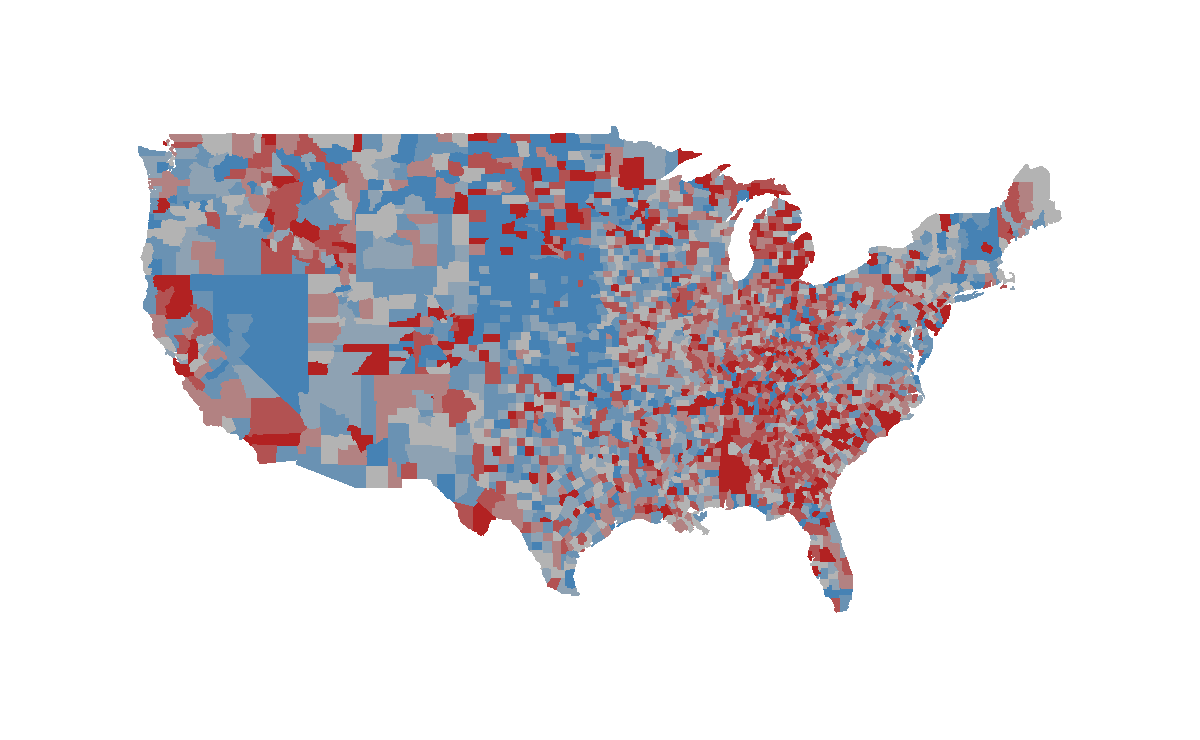
\includegraphics[width=0.7\linewidth]{DS4PS-I_files/figure-latex/unnamed-chunk-131-2} 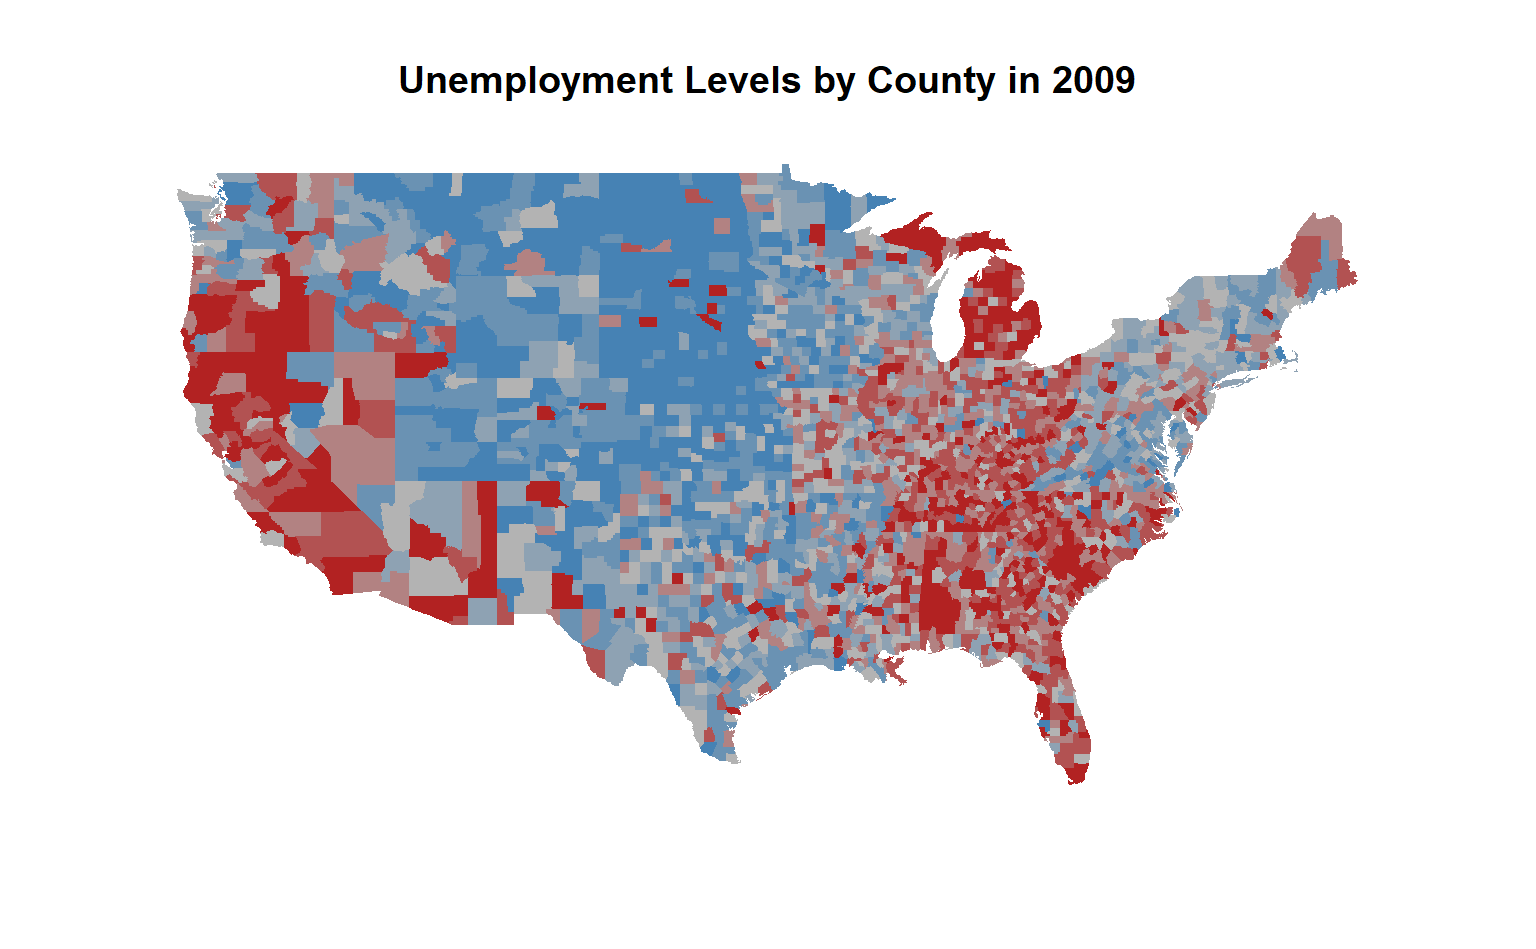
\includegraphics[width=0.7\linewidth]{DS4PS-I_files/figure-latex/unnamed-chunk-131-3} \end{center}

Note that elements can be recycled from your \emph{y} vector:

\begin{Shaded}
\begin{Highlighting}[]

\NormalTok{x <-}\StringTok{ }\KeywordTok{c}\NormalTok{(}\StringTok{"A"}\NormalTok{,}\StringTok{"B"}\NormalTok{,}\StringTok{"C"}\NormalTok{,}\StringTok{"B"}\NormalTok{)}

\NormalTok{y <-}\StringTok{ }\KeywordTok{c}\NormalTok{(}\StringTok{"B"}\NormalTok{,}\StringTok{"D"}\NormalTok{,}\StringTok{"A"}\NormalTok{,}\StringTok{"F"}\NormalTok{)}

\KeywordTok{cbind}\NormalTok{( x, y )}
\CommentTok{###      x   y  }
\CommentTok{### [1,] "A" "B"}
\CommentTok{### [2,] "B" "D"}
\CommentTok{### [3,] "C" "A"}
\CommentTok{### [4,] "B" "F"}

\KeywordTok{match}\NormalTok{( x, y )}
\CommentTok{### [1]  3  1 NA  1}

\NormalTok{order.y <-}\StringTok{ }\KeywordTok{match}\NormalTok{( x, y )}

\NormalTok{y.new <-}\StringTok{ }\NormalTok{y[ order.y ]}

\KeywordTok{cbind}\NormalTok{( x, y.new )}
\CommentTok{###      x   y.new}
\CommentTok{### [1,] "A" "A"  }
\CommentTok{### [2,] "B" "B"  }
\CommentTok{### [3,] "C" NA   }
\CommentTok{### [4,] "B" "B"}
\end{Highlighting}
\end{Shaded}

\hypertarget{analysis-with-groups-in-r}{%
\chapter{Analysis with Groups in R}\label{analysis-with-groups-in-r}}

\hypertarget{packages-used-in-this-chapter-1}{%
\subsection{Packages Used in this
Chapter}\label{packages-used-in-this-chapter-1}}

\begin{Shaded}
\begin{Highlighting}[]

\KeywordTok{library}\NormalTok{( pander )}
\KeywordTok{library}\NormalTok{( dplyr )}
\KeywordTok{library}\NormalTok{( tidyr )}
\KeywordTok{library}\NormalTok{( reshape2 )}
\KeywordTok{library}\NormalTok{( scales )}
\KeywordTok{library}\NormalTok{( ggplot2 )}
\KeywordTok{library}\NormalTok{( Lahman )}
\end{Highlighting}
\end{Shaded}

\hypertarget{hypothetical-experimental-data}{%
\subsection{Hypothetical Experimental
Data}\label{hypothetical-experimental-data}}

We will demonstrate some functions using this hypothetical dataset:

\begin{Shaded}
\begin{Highlighting}[]
\KeywordTok{head}\NormalTok{( d ) }\OperatorTok\StringTok{ }\NormalTok{pander}
\end{Highlighting}
\end{Shaded}

\begin{longtable}[]{@{}ccccccc@{}}
\toprule
\begin{minipage}[b]{0.06\columnwidth}\centering
id\strut
\end{minipage} & \begin{minipage}[b]{0.09\columnwidth}\centering
race\strut
\end{minipage} & \begin{minipage}[b]{0.15\columnwidth}\centering
blood.type\strut
\end{minipage} & \begin{minipage}[b]{0.10\columnwidth}\centering
gender\strut
\end{minipage} & \begin{minipage}[b]{0.07\columnwidth}\centering
age\strut
\end{minipage} & \begin{minipage}[b]{0.16\columnwidth}\centering
study.group\strut
\end{minipage} & \begin{minipage}[b]{0.09\columnwidth}\centering
speed\strut
\end{minipage}\tabularnewline
\midrule
\endhead
\begin{minipage}[t]{0.06\columnwidth}\centering
1\strut
\end{minipage} & \begin{minipage}[t]{0.09\columnwidth}\centering
white\strut
\end{minipage} & \begin{minipage}[t]{0.15\columnwidth}\centering
B\strut
\end{minipage} & \begin{minipage}[t]{0.10\columnwidth}\centering
female\strut
\end{minipage} & \begin{minipage}[t]{0.07\columnwidth}\centering
34\strut
\end{minipage} & \begin{minipage}[t]{0.16\columnwidth}\centering
treatment\strut
\end{minipage} & \begin{minipage}[t]{0.09\columnwidth}\centering
628\strut
\end{minipage}\tabularnewline
\begin{minipage}[t]{0.06\columnwidth}\centering
2\strut
\end{minipage} & \begin{minipage}[t]{0.09\columnwidth}\centering
black\strut
\end{minipage} & \begin{minipage}[t]{0.15\columnwidth}\centering
B\strut
\end{minipage} & \begin{minipage}[t]{0.10\columnwidth}\centering
female\strut
\end{minipage} & \begin{minipage}[t]{0.07\columnwidth}\centering
44\strut
\end{minipage} & \begin{minipage}[t]{0.16\columnwidth}\centering
treatment\strut
\end{minipage} & \begin{minipage}[t]{0.09\columnwidth}\centering
654.2\strut
\end{minipage}\tabularnewline
\begin{minipage}[t]{0.06\columnwidth}\centering
3\strut
\end{minipage} & \begin{minipage}[t]{0.09\columnwidth}\centering
black\strut
\end{minipage} & \begin{minipage}[t]{0.15\columnwidth}\centering
A\strut
\end{minipage} & \begin{minipage}[t]{0.10\columnwidth}\centering
female\strut
\end{minipage} & \begin{minipage}[t]{0.07\columnwidth}\centering
55\strut
\end{minipage} & \begin{minipage}[t]{0.16\columnwidth}\centering
treatment\strut
\end{minipage} & \begin{minipage}[t]{0.09\columnwidth}\centering
566.2\strut
\end{minipage}\tabularnewline
\begin{minipage}[t]{0.06\columnwidth}\centering
4\strut
\end{minipage} & \begin{minipage}[t]{0.09\columnwidth}\centering
white\strut
\end{minipage} & \begin{minipage}[t]{0.15\columnwidth}\centering
A\strut
\end{minipage} & \begin{minipage}[t]{0.10\columnwidth}\centering
female\strut
\end{minipage} & \begin{minipage}[t]{0.07\columnwidth}\centering
46\strut
\end{minipage} & \begin{minipage}[t]{0.16\columnwidth}\centering
treatment\strut
\end{minipage} & \begin{minipage}[t]{0.09\columnwidth}\centering
701.3\strut
\end{minipage}\tabularnewline
\begin{minipage}[t]{0.06\columnwidth}\centering
5\strut
\end{minipage} & \begin{minipage}[t]{0.09\columnwidth}\centering
black\strut
\end{minipage} & \begin{minipage}[t]{0.15\columnwidth}\centering
A\strut
\end{minipage} & \begin{minipage}[t]{0.10\columnwidth}\centering
male\strut
\end{minipage} & \begin{minipage}[t]{0.07\columnwidth}\centering
43\strut
\end{minipage} & \begin{minipage}[t]{0.16\columnwidth}\centering
treatment\strut
\end{minipage} & \begin{minipage}[t]{0.09\columnwidth}\centering
596.8\strut
\end{minipage}\tabularnewline
\begin{minipage}[t]{0.06\columnwidth}\centering
6\strut
\end{minipage} & \begin{minipage}[t]{0.09\columnwidth}\centering
black\strut
\end{minipage} & \begin{minipage}[t]{0.15\columnwidth}\centering
A\strut
\end{minipage} & \begin{minipage}[t]{0.10\columnwidth}\centering
male\strut
\end{minipage} & \begin{minipage}[t]{0.07\columnwidth}\centering
32\strut
\end{minipage} & \begin{minipage}[t]{0.16\columnwidth}\centering
treatment\strut
\end{minipage} & \begin{minipage}[t]{0.09\columnwidth}\centering
549.6\strut
\end{minipage}\tabularnewline
\bottomrule
\end{longtable}

\hypertarget{group-structure}{%
\section{Group Structure}\label{group-structure}}

The two most important skills as you first learn a data programming
language are:

\begin{enumerate}
\def\labelenumi{\arabic{enumi}.}
\tightlist
\item
  Translating English phrases into computer code using logical
  statements\\
\item
  Organizing your data into groups
\end{enumerate}

This lecture focuses on efficienty splitting your data into groups, and
then analyzing your data by group.

\hypertarget{what-are-groups}{%
\subsection{What Are Groups?}\label{what-are-groups}}

A group represents a set of elements with identical characteristics -
mice all belong to one group and elephants belong to another. Easy
enough, right?

In data analysis, it is a little more complicated because a group is
defined by a set of features. Each group still represents a set of
elements with identical characteristics, but when we have multiple
features there is a unique group for each combination of features.

The simple way to think about this is that the cross-tab of features
generates a grid (table), and each cell represents a unique group:

\begin{center}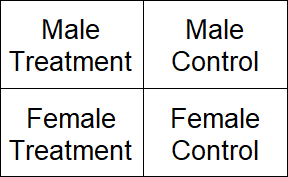
\includegraphics[width=0.7\linewidth]{DS4PS-I_files/figure-latex/unnamed-chunk-138-1} \end{center}

We might be interested in simple groups (treatment cases versus control
cases), or complex groups (does the treatment effect women and men
differently?).

In previous lectures you have learned to identify a group with a logical
statement, and analyze that group discretely.

\begin{Shaded}
\begin{Highlighting}[]

\KeywordTok{mean}\NormalTok{( speed[ study.group }\OperatorTok{==}\StringTok{ "treatment"} \OperatorTok{&}\StringTok{ }\NormalTok{gender}\OperatorTok{==}\StringTok{"female"}\NormalTok{ ] )}
\CommentTok{### [1] 612.6091}
\end{Highlighting}
\end{Shaded}

In this lecture you will learn to define a group structure, then analyze
all of your data using that structure.

\begin{Shaded}
\begin{Highlighting}[]

\KeywordTok{tapply}\NormalTok{( speed, }\DataTypeTok{INDEX =} \KeywordTok{list}\NormalTok{( study.group, gender ), }\DataTypeTok{FUN =}\NormalTok{ mean )}
\end{Highlighting}
\end{Shaded}

\begin{longtable}[]{@{}ccc@{}}
\toprule
\begin{minipage}[b]{0.20\columnwidth}\centering
~\strut
\end{minipage} & \begin{minipage}[b]{0.11\columnwidth}\centering
female\strut
\end{minipage} & \begin{minipage}[b]{0.11\columnwidth}\centering
male\strut
\end{minipage}\tabularnewline
\midrule
\endhead
\begin{minipage}[t]{0.20\columnwidth}\centering
\textbf{control}\strut
\end{minipage} & \begin{minipage}[t]{0.11\columnwidth}\centering
453.8\strut
\end{minipage} & \begin{minipage}[t]{0.11\columnwidth}\centering
363.7\strut
\end{minipage}\tabularnewline
\begin{minipage}[t]{0.20\columnwidth}\centering
\textbf{treatment}\strut
\end{minipage} & \begin{minipage}[t]{0.11\columnwidth}\centering
612.6\strut
\end{minipage} & \begin{minipage}[t]{0.11\columnwidth}\centering
515.4\strut
\end{minipage}\tabularnewline
\bottomrule
\end{longtable}

\hypertarget{main-take-away}{%
\subsection{Main Take-Away}\label{main-take-away}}

R has been designed to do efficient data analysis by defining a group
structure, then quickly applying a function to all unique members.

The base R packages do this with a set of functions in the
\textbf{apply()} family. The \textbf{tapply()} function allows you to
specify an outcome to analyze and a group, then ask for results from a
function.

\begin{Shaded}
\begin{Highlighting}[]

\KeywordTok{tapply}\NormalTok{( }\DataTypeTok{X=}\NormalTok{speed, }\DataTypeTok{INDEX=}\KeywordTok{list}\NormalTok{( study.group, gender ), }\DataTypeTok{FUN=}\NormalTok{mean ) }
\end{Highlighting}
\end{Shaded}

\begin{longtable}[]{@{}ccc@{}}
\toprule
\begin{minipage}[b]{0.20\columnwidth}\centering
~\strut
\end{minipage} & \begin{minipage}[b]{0.11\columnwidth}\centering
female\strut
\end{minipage} & \begin{minipage}[b]{0.11\columnwidth}\centering
male\strut
\end{minipage}\tabularnewline
\midrule
\endhead
\begin{minipage}[t]{0.20\columnwidth}\centering
\textbf{control}\strut
\end{minipage} & \begin{minipage}[t]{0.11\columnwidth}\centering
453.8\strut
\end{minipage} & \begin{minipage}[t]{0.11\columnwidth}\centering
363.7\strut
\end{minipage}\tabularnewline
\begin{minipage}[t]{0.20\columnwidth}\centering
\textbf{treatment}\strut
\end{minipage} & \begin{minipage}[t]{0.11\columnwidth}\centering
612.6\strut
\end{minipage} & \begin{minipage}[t]{0.11\columnwidth}\centering
515.4\strut
\end{minipage}\tabularnewline
\bottomrule
\end{longtable}

The \textbf{dplyr} package makes this process easier using some simple
verbs and the ``pipe'' operator.

\begin{Shaded}
\begin{Highlighting}[]

\NormalTok{dat  }\OperatorTok\StringTok{  }\KeywordTok{group_by}\NormalTok{( study.group, gender )  }\OperatorTok\StringTok{  }\KeywordTok{summarize}\NormalTok{( }\DataTypeTok{ave.speed =} \KeywordTok{mean}\NormalTok{(speed) )}
\end{Highlighting}
\end{Shaded}

\begin{longtable}[]{@{}ccc@{}}
\toprule
\begin{minipage}[b]{0.18\columnwidth}\centering
study.group\strut
\end{minipage} & \begin{minipage}[b]{0.11\columnwidth}\centering
gender\strut
\end{minipage} & \begin{minipage}[b]{0.15\columnwidth}\centering
ave.speed\strut
\end{minipage}\tabularnewline
\midrule
\endhead
\begin{minipage}[t]{0.18\columnwidth}\centering
control\strut
\end{minipage} & \begin{minipage}[t]{0.11\columnwidth}\centering
male\strut
\end{minipage} & \begin{minipage}[t]{0.15\columnwidth}\centering
363.7\strut
\end{minipage}\tabularnewline
\begin{minipage}[t]{0.18\columnwidth}\centering
control\strut
\end{minipage} & \begin{minipage}[t]{0.11\columnwidth}\centering
female\strut
\end{minipage} & \begin{minipage}[t]{0.15\columnwidth}\centering
453.8\strut
\end{minipage}\tabularnewline
\begin{minipage}[t]{0.18\columnwidth}\centering
treatment\strut
\end{minipage} & \begin{minipage}[t]{0.11\columnwidth}\centering
male\strut
\end{minipage} & \begin{minipage}[t]{0.15\columnwidth}\centering
515.4\strut
\end{minipage}\tabularnewline
\begin{minipage}[t]{0.18\columnwidth}\centering
treatment\strut
\end{minipage} & \begin{minipage}[t]{0.11\columnwidth}\centering
female\strut
\end{minipage} & \begin{minipage}[t]{0.15\columnwidth}\centering
612.6\strut
\end{minipage}\tabularnewline
\bottomrule
\end{longtable}

\hypertarget{example}{%
\subsection{Example}\label{example}}

Let's think about a study looking at reading speed. The treatment is a
workshop that teaches some speed-reading techniques. In this study we
have data on:

\begin{itemize}
\tightlist
\item
  gender (male,female)
\item
  race (black,white,asian)
\item
  blood.type (A,B)
\item
  age (from 18 to 93)
\end{itemize}

Examining descriptive statistics we can see that reading speed varies by
gender and the treatment group, but not by race or blood type:

\begin{center}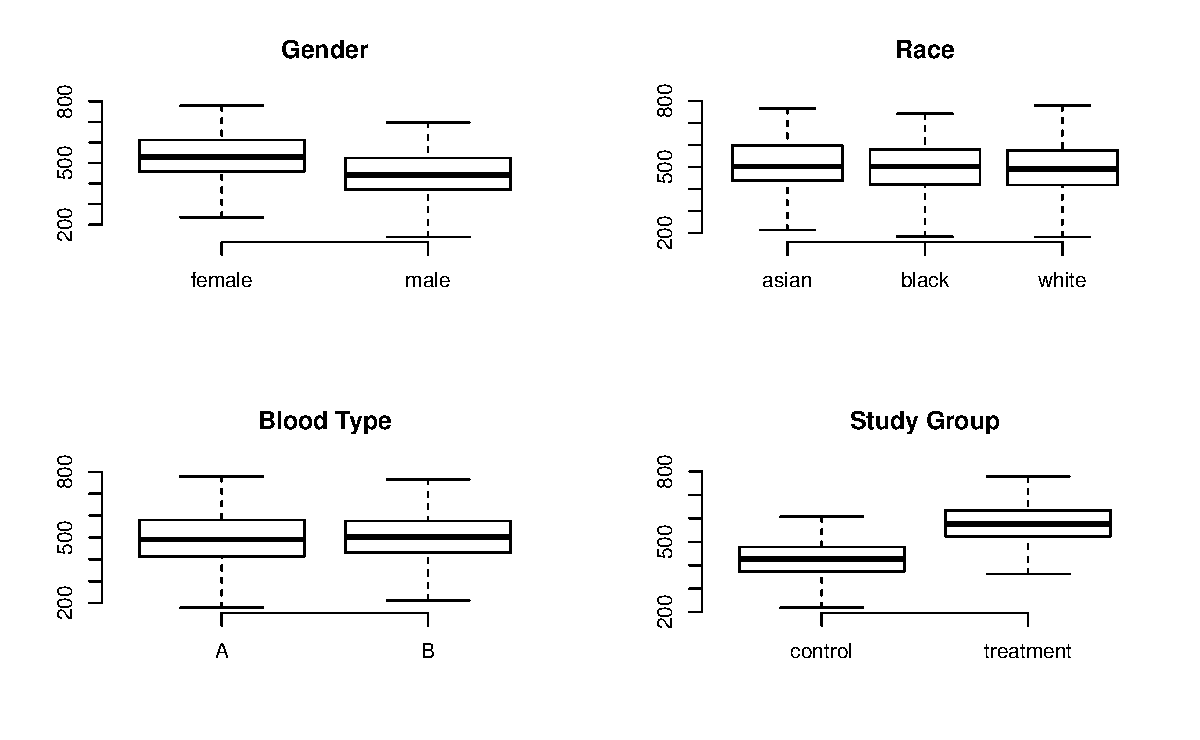
\includegraphics[width=0.7\linewidth]{DS4PS-I_files/figure-latex/unnamed-chunk-147-1} \end{center}

The question is, how many unique groups can we create with these four
factors?

Each individual factor contains a small number of levels (only 2 or 3 in
this case), which makes the group structure look deceptively simple at
first glance. When we start to examine combinations of factors we see
that group structure can get complicated pretty quickly.

If we look at gender alone, we have two levels: male and female. So we
have two groups. If we look at our study groups alone we have two
groups: treatment and control.

If we look at gender and the study groups together, we now have a 2 x 2
grid, or four unique groups.

If the race factor has three levels, how many unique groups will we have
considering the study design, gender, and race together?

\begin{center}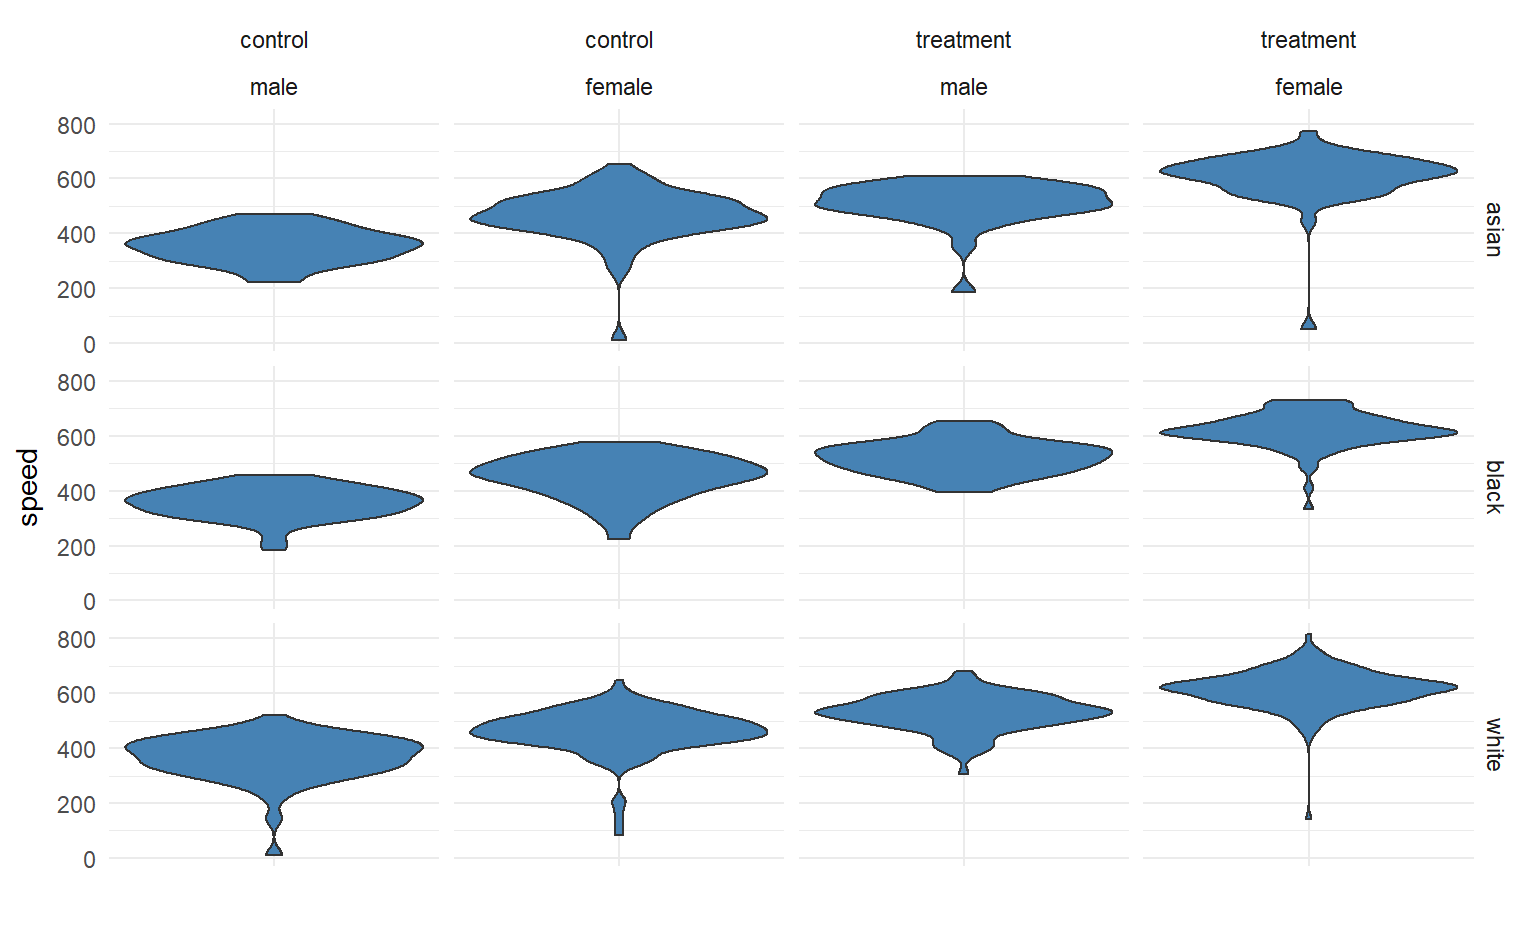
\includegraphics[width=0.7\linewidth]{DS4PS-I_files/figure-latex/unnamed-chunk-148-1} \end{center}

We can calculate the size of the grid by multiplying number of levels
for each factor. We see here we have 12 unique groups:

\begin{Shaded}
\begin{Highlighting}[]

\KeywordTok{nlevels}\NormalTok{( gender ) }\OperatorTok{*}\StringTok{ }\KeywordTok{nlevels}\NormalTok{( study.group ) }\OperatorTok{*}\StringTok{ }\KeywordTok{nlevels}\NormalTok{( race )}
\CommentTok{### [1] 12}
\end{Highlighting}
\end{Shaded}

If we add blood type, a factor with two levels (A and B), we now have 24
unique groups:

\begin{Shaded}
\begin{Highlighting}[]

\NormalTok{p }\OperatorTok{+}\StringTok{ }\KeywordTok{facet_grid}\NormalTok{( race }\OperatorTok{+}\StringTok{ }\NormalTok{study.group }\OperatorTok{~}\StringTok{ }\NormalTok{gender }\OperatorTok{+}\StringTok{ }\NormalTok{blood.type) }
\end{Highlighting}
\end{Shaded}

\begin{center}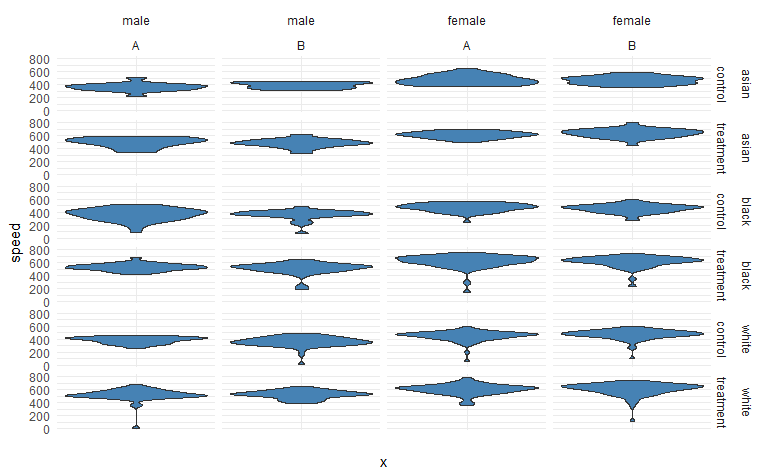
\includegraphics[width=0.7\linewidth]{DS4PS-I_files/figure-latex/unnamed-chunk-150-1} \end{center}

What about age? It is a continuous variable, so it's a little more
tricky.

We can certainly analyze the relationship between age and speed using
correlation tools.

\begin{Shaded}
\begin{Highlighting}[]
\KeywordTok{plot}\NormalTok{( age, speed, }\DataTypeTok{bty=}\StringTok{"n"}\NormalTok{, }\DataTypeTok{main=}\StringTok{"Age"}\NormalTok{ )}
\end{Highlighting}
\end{Shaded}

\begin{center}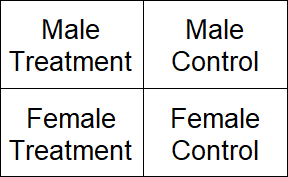
\includegraphics[width=0.7\linewidth]{DS4PS-I_files/figure-latex/unnamed-chunk-151-1} \end{center}

But we can also incorporate this independent variable into a group
structure. We can treat each distinct age as a separate group. The ages
in this study range from 18 to 93, so we have 65 distinct ages
represented.

\begin{Shaded}
\begin{Highlighting}[]

\KeywordTok{plot}\NormalTok{( }\KeywordTok{factor}\NormalTok{(age), speed, }\DataTypeTok{las=}\DecValTok{2}\NormalTok{, }\DataTypeTok{frame.plot=}\NormalTok{F, }\DataTypeTok{outline=}\NormalTok{F, }\DataTypeTok{main=}\StringTok{"Age"}\NormalTok{, }\DataTypeTok{xaxt=}\StringTok{"n"}\NormalTok{  )}
\end{Highlighting}
\end{Shaded}

\begin{center}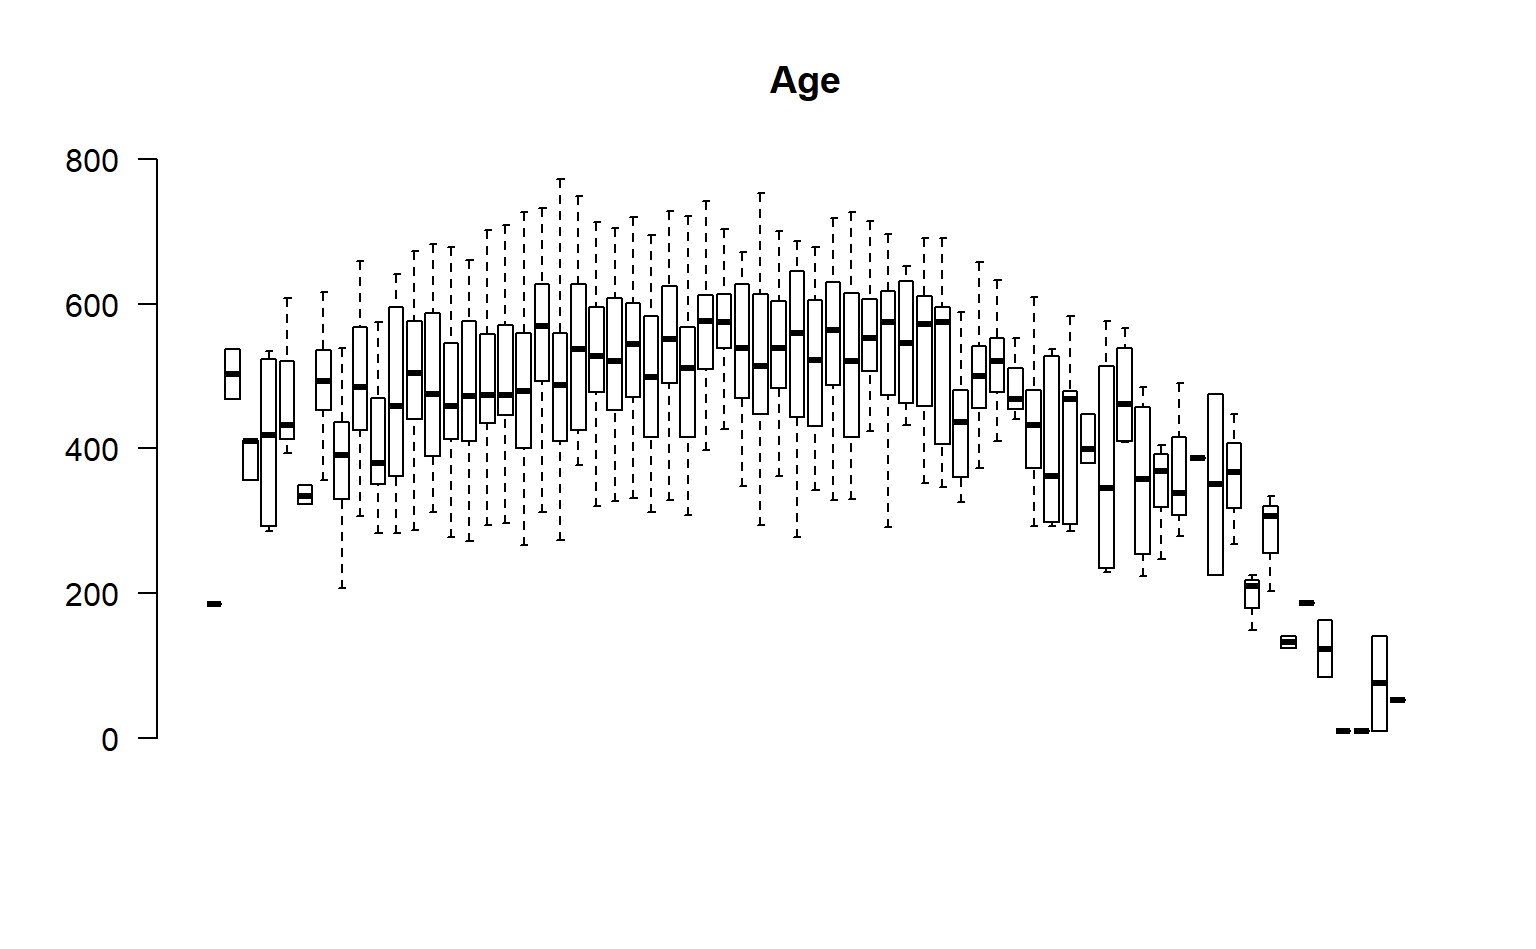
\includegraphics[width=0.7\linewidth]{DS4PS-I_files/figure-latex/unnamed-chunk-152-1} \end{center}

If we think about the overall group structure, then, we have unique
groups defined by gender, race, blood type, and study design, and
another 65 age groups. So in total we now have 24 x 65 = 1,560 groups!
That is getting complicated.

This group design is problematic for two reasons. From a pragmatic
standpoint, we can't report results from 1,500 groups in a table. From a
more substantive perspective, we although we have 1,500 distinct cells
in our grid, many may not include observations that represent the unique
combination of all factors. So this group design is not very practical.

A similar problem arises if our data includes time. If our data includes
the time of events recorded by hours, days of the week, months, and
years, we can have generate complicated group structures if we try to
analyze every unique combination.

We can simplify our analysis by thinking about age ranges instead of
ages, or in other words by binning our continuous data. If we split it
into five-year ranges, for example, we have gone from 65 distinct ages
to 12 distinct age groups.

\begin{Shaded}
\begin{Highlighting}[]

\NormalTok{age.group <-}\StringTok{ }\KeywordTok{cut}\NormalTok{( age, }
                  \DataTypeTok{breaks=}\KeywordTok{seq}\NormalTok{(}\DataTypeTok{from=}\DecValTok{20}\NormalTok{,}\DataTypeTok{to=}\DecValTok{80}\NormalTok{,}\DataTypeTok{by=}\DecValTok{5}\NormalTok{),}
                  \DataTypeTok{labels=}\KeywordTok{paste}\NormalTok{( }\KeywordTok{seq}\NormalTok{(}\DataTypeTok{from=}\DecValTok{20}\NormalTok{,}\DataTypeTok{to=}\DecValTok{75}\NormalTok{,}\DataTypeTok{by=}\DecValTok{5}\NormalTok{), }\StringTok{"to"}\NormalTok{, }\KeywordTok{seq}\NormalTok{(}\DataTypeTok{from=}\DecValTok{25}\NormalTok{,}\DataTypeTok{to=}\DecValTok{80}\NormalTok{,}\DataTypeTok{by=}\DecValTok{5}\NormalTok{) ) )}

\NormalTok{group.structure <-}\StringTok{ }\KeywordTok{formula}\NormalTok{( speed }\OperatorTok{~}\StringTok{ }\NormalTok{age.group )}

\KeywordTok{boxplot}\NormalTok{( group.structure, }\DataTypeTok{las=}\DecValTok{2}\NormalTok{, }\DataTypeTok{frame.plot=}\NormalTok{F, }\DataTypeTok{outline=}\NormalTok{F, }\DataTypeTok{main=}\StringTok{"Age Group"}\NormalTok{  )}
\end{Highlighting}
\end{Shaded}

\begin{center}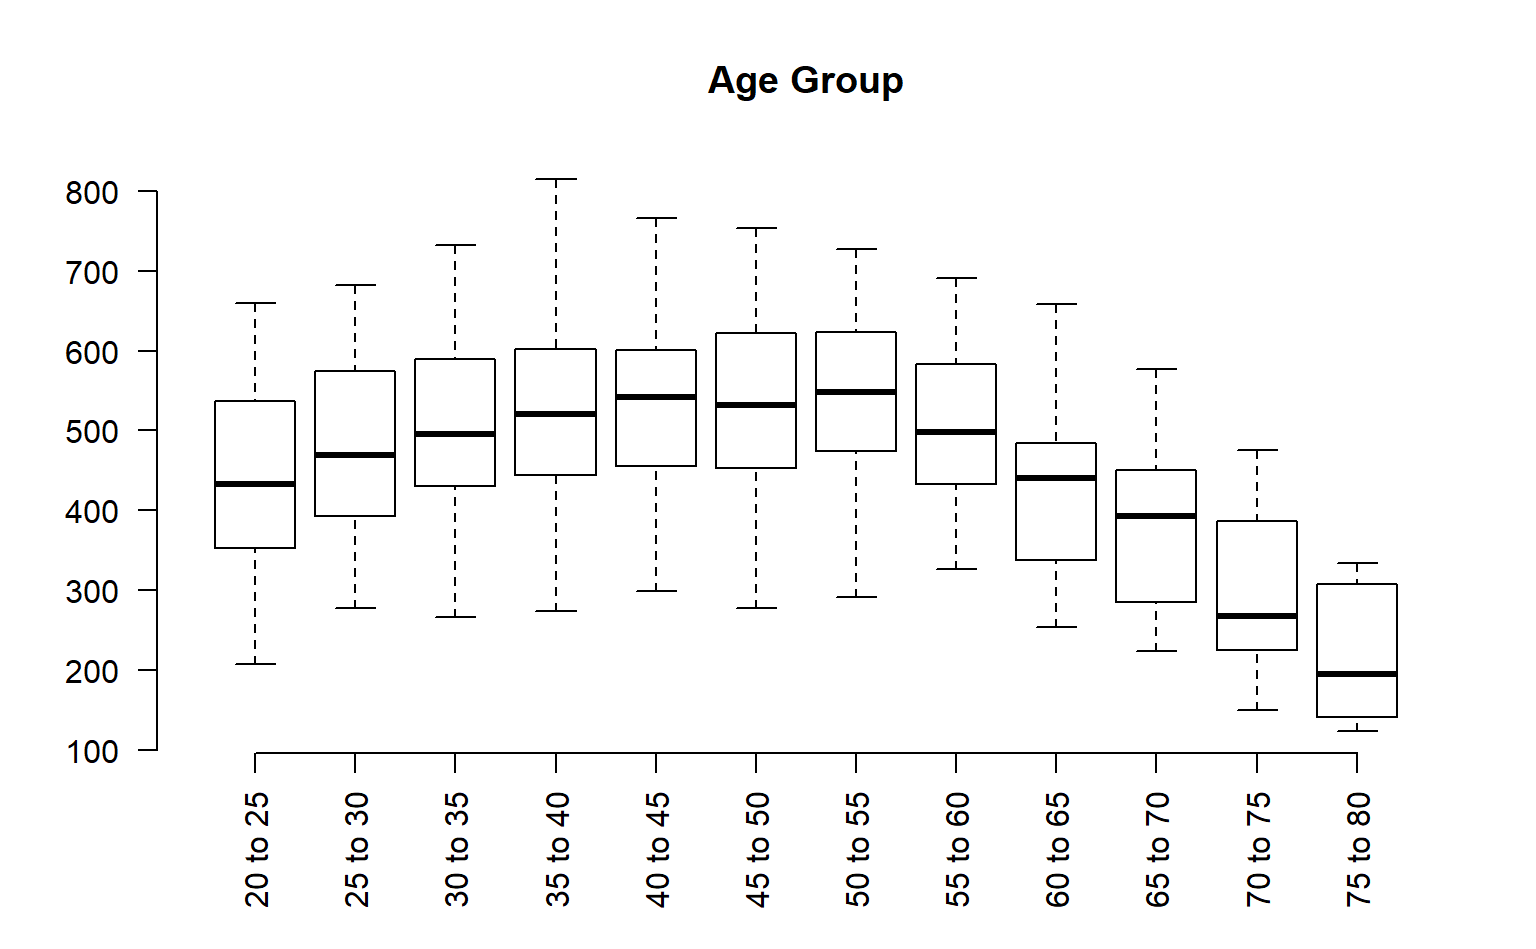
\includegraphics[width=0.7\linewidth]{DS4PS-I_files/figure-latex/unnamed-chunk-153-1} \end{center}

We have now simplified our analysis from 1,560 to 288 possible groups.
Combinations of groups will also be easier:

\begin{Shaded}
\begin{Highlighting}[]

\NormalTok{group.structure <-}\StringTok{ }\KeywordTok{formula}\NormalTok{( speed }\OperatorTok{~}\StringTok{ }\NormalTok{gender }\OperatorTok{*}\StringTok{ }\NormalTok{age.group )}

\KeywordTok{boxplot}\NormalTok{( group.structure, }
         \DataTypeTok{las=}\DecValTok{2}\NormalTok{, }\DataTypeTok{frame.plot=}\NormalTok{F, }\DataTypeTok{outline=}\NormalTok{F, }\DataTypeTok{main=}\StringTok{"Age Group by Gender"}\NormalTok{,}
         \DataTypeTok{col=}\KeywordTok{c}\NormalTok{(}\StringTok{"firebrick"}\NormalTok{,}\StringTok{"steelblue"}\NormalTok{), }\DataTypeTok{xaxt=}\StringTok{"n"}\NormalTok{ )}
\end{Highlighting}
\end{Shaded}

\begin{center}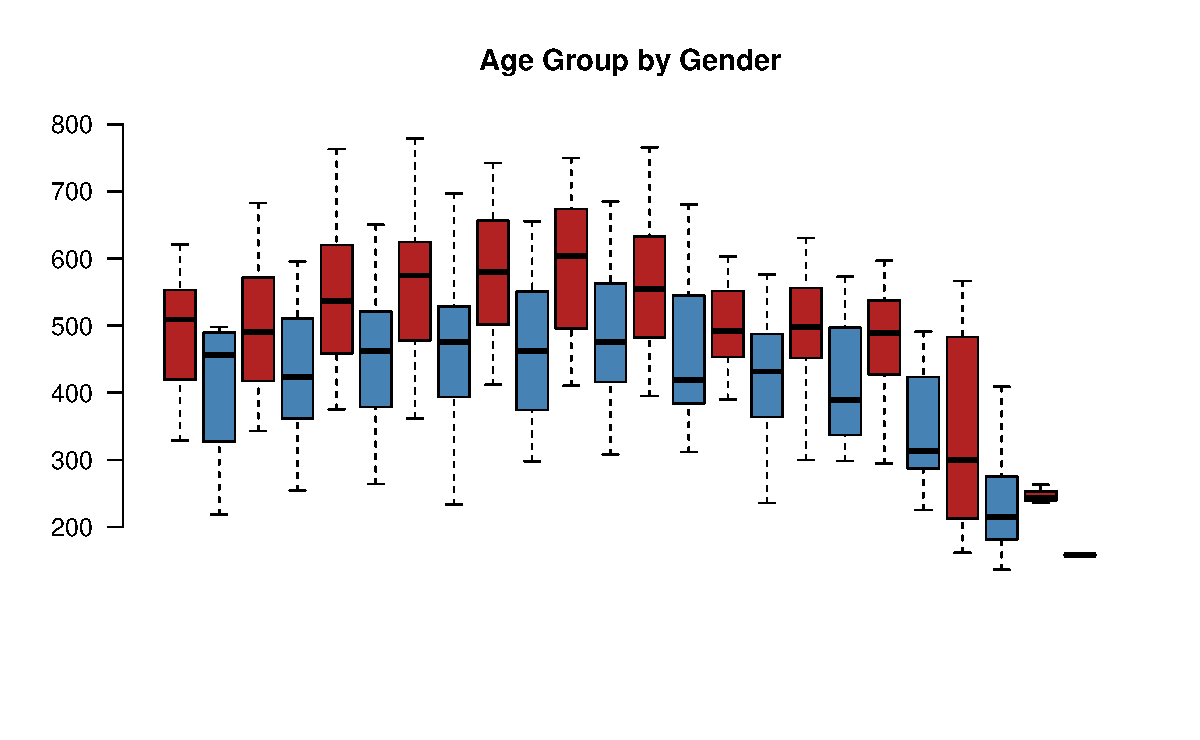
\includegraphics[width=0.7\linewidth]{DS4PS-I_files/figure-latex/unnamed-chunk-154-1} \end{center}

\hypertarget{analysis-by-group}{%
\section{Analysis by Group}\label{analysis-by-group}}

Let's demonstrate some analysis of groups using the Lahman package and
some \textbf{dplyr} verbs. Let's do some analysis of player salaries
(\emph{Salaries} dataset), and start with a simple group structure -
teams in the National League and time.

\begin{enumerate}
\def\labelenumi{\arabic{enumi}.}
\tightlist
\item
  Which team has the highest average player salary?
\item
  Which team has the most players paid over \$5 million a season?
\item
  Which team has raised it's pay the most over the past decade?
\end{enumerate}

Let's start by thinking about group structure. We have teams, and we
have seasons. Teams is stored as a factor, and seasons as a numeric
value, so we can consider group for each by counting levels and unique
values:

\begin{Shaded}
\begin{Highlighting}[]
\KeywordTok{nlevels}\NormalTok{( Salaries}\OperatorTok{$}\NormalTok{teamID )}
\CommentTok{### [1] 46}
\KeywordTok{length}\NormalTok{( }\KeywordTok{unique}\NormalTok{( Salaries}\OperatorTok{$}\NormalTok{yearID ) )}
\CommentTok{### [1] 32}
\end{Highlighting}
\end{Shaded}

So we can potentially calculate 32 x 46 = 1,472 average player salaries.

\hypertarget{highest-ave-player-salary}{%
\subsection{Highest Ave Player Salary}\label{highest-ave-player-salary}}

For our first question, we will select only teams from the National
League. Let's use the most recent year of data to calculate average pay.

\begin{Shaded}
\begin{Highlighting}[]

\NormalTok{Salaries }\OperatorTok\StringTok{ }\KeywordTok{filter}\NormalTok{( lgID }\OperatorTok{==}\StringTok{ "NL"}\NormalTok{, yearID }\OperatorTok{==}\StringTok{ }\DecValTok{2016}\NormalTok{ ) }\OperatorTok\StringTok{ }
\StringTok{             }\KeywordTok{group_by}\NormalTok{( teamID) }\OperatorTok\StringTok{ }
\StringTok{             }\KeywordTok{summarize}\NormalTok{( }\DataTypeTok{Ave_Salary =} \KeywordTok{mean}\NormalTok{(salary) )}
\CommentTok{### # A tibble: 15 x 2}
\CommentTok{###   teamID Ave_Salary}
\CommentTok{###   <fct>       <dbl>}
\CommentTok{### 1 ARI      3363041.}
\CommentTok{### 2 ATL      2362010.}
\CommentTok{### 3 CHC      5312678.}
\CommentTok{### 4 CIN      3066899.}
\CommentTok{### 5 COL      3413487 }
\CommentTok{### 6 LAD      6322525.}
\CommentTok{### # ... with 9 more rows}
\end{Highlighting}
\end{Shaded}

Since the salaries are large, they are a little hard to read. Let's
clean up the table a bit.

\begin{Shaded}
\begin{Highlighting}[]


\NormalTok{Salaries  }\OperatorTok\StringTok{ }
\StringTok{             }\KeywordTok{filter}\NormalTok{( lgID }\OperatorTok{==}\StringTok{ "NL"}\NormalTok{, yearID }\OperatorTok{==}\StringTok{ }\DecValTok{2016}\NormalTok{ ) }\OperatorTok\StringTok{ }
\StringTok{             }\KeywordTok{group_by}\NormalTok{( teamID ) }\OperatorTok\StringTok{ }
\StringTok{             }\KeywordTok{summarize}\NormalTok{( }\DataTypeTok{Ave_Salary=}\KeywordTok{dollar}\NormalTok{( }\KeywordTok{mean}\NormalTok{(salary,}\DataTypeTok{na.rm=}\NormalTok{T) ) ) }\OperatorTok
\StringTok{             }\KeywordTok{arrange}\NormalTok{( }\KeywordTok{desc}\NormalTok{(Ave_Salary) ) }\OperatorTok
\StringTok{             }\KeywordTok{pander}\NormalTok{()}
\end{Highlighting}
\end{Shaded}

\begin{longtable}[]{@{}cc@{}}
\toprule
\begin{minipage}[b]{0.12\columnwidth}\centering
teamID\strut
\end{minipage} & \begin{minipage}[b]{0.17\columnwidth}\centering
Ave\_Salary\strut
\end{minipage}\tabularnewline
\midrule
\endhead
\begin{minipage}[t]{0.12\columnwidth}\centering
SFG\strut
\end{minipage} & \begin{minipage}[t]{0.17\columnwidth}\centering
\$6,890,151\strut
\end{minipage}\tabularnewline
\begin{minipage}[t]{0.12\columnwidth}\centering
LAD\strut
\end{minipage} & \begin{minipage}[t]{0.17\columnwidth}\centering
\$6,322,525\strut
\end{minipage}\tabularnewline
\begin{minipage}[t]{0.12\columnwidth}\centering
WSN\strut
\end{minipage} & \begin{minipage}[t]{0.17\columnwidth}\centering
\$5,448,179\strut
\end{minipage}\tabularnewline
\begin{minipage}[t]{0.12\columnwidth}\centering
CHC\strut
\end{minipage} & \begin{minipage}[t]{0.17\columnwidth}\centering
\$5,312,678\strut
\end{minipage}\tabularnewline
\begin{minipage}[t]{0.12\columnwidth}\centering
NYM\strut
\end{minipage} & \begin{minipage}[t]{0.17\columnwidth}\centering
\$4,958,857\strut
\end{minipage}\tabularnewline
\begin{minipage}[t]{0.12\columnwidth}\centering
STL\strut
\end{minipage} & \begin{minipage}[t]{0.17\columnwidth}\centering
\$4,614,629\strut
\end{minipage}\tabularnewline
\begin{minipage}[t]{0.12\columnwidth}\centering
SDP\strut
\end{minipage} & \begin{minipage}[t]{0.17\columnwidth}\centering
\$3,756,475\strut
\end{minipage}\tabularnewline
\begin{minipage}[t]{0.12\columnwidth}\centering
PIT\strut
\end{minipage} & \begin{minipage}[t]{0.17\columnwidth}\centering
\$3,706,387\strut
\end{minipage}\tabularnewline
\begin{minipage}[t]{0.12\columnwidth}\centering
COL\strut
\end{minipage} & \begin{minipage}[t]{0.17\columnwidth}\centering
\$3,413,487\strut
\end{minipage}\tabularnewline
\begin{minipage}[t]{0.12\columnwidth}\centering
ARI\strut
\end{minipage} & \begin{minipage}[t]{0.17\columnwidth}\centering
\$3,363,041\strut
\end{minipage}\tabularnewline
\begin{minipage}[t]{0.12\columnwidth}\centering
CIN\strut
\end{minipage} & \begin{minipage}[t]{0.17\columnwidth}\centering
\$3,066,899\strut
\end{minipage}\tabularnewline
\begin{minipage}[t]{0.12\columnwidth}\centering
MIA\strut
\end{minipage} & \begin{minipage}[t]{0.17\columnwidth}\centering
\$2,761,222\strut
\end{minipage}\tabularnewline
\begin{minipage}[t]{0.12\columnwidth}\centering
ATL\strut
\end{minipage} & \begin{minipage}[t]{0.17\columnwidth}\centering
\$2,362,010\strut
\end{minipage}\tabularnewline
\begin{minipage}[t]{0.12\columnwidth}\centering
MIL\strut
\end{minipage} & \begin{minipage}[t]{0.17\columnwidth}\centering
\$2,292,508\strut
\end{minipage}\tabularnewline
\begin{minipage}[t]{0.12\columnwidth}\centering
PHI\strut
\end{minipage} & \begin{minipage}[t]{0.17\columnwidth}\centering
\$2,033,793\strut
\end{minipage}\tabularnewline
\bottomrule
\end{longtable}

\hypertarget{most-players-paid-over-5-million}{%
\subsection{Most Players Paid Over \$5
Million}\label{most-players-paid-over-5-million}}

This question requires you to utilize a logical statement in order to
translate from the question to code. We need to inspect each salary,
determine whether it is over the \$5m threshold, then count all of the
cases. The operation will look something like this:

\begin{Shaded}
\begin{Highlighting}[]
\KeywordTok{sum}\NormalTok{( Salaries}\OperatorTok{$}\NormalTok{salary }\OperatorTok{>}\StringTok{ }\DecValTok{5000000}\NormalTok{ )}
\CommentTok{### [1] 3175}
\end{Highlighting}
\end{Shaded}

It gets a little trickier when we want to do the operation
simultaneously across groups. Our team group structure is already
defined, so let's define our logical vector and count cases that match:

\begin{Shaded}
\begin{Highlighting}[]

\NormalTok{dat.NL <-}\StringTok{ }\KeywordTok{filter}\NormalTok{( Salaries, yearID }\OperatorTok{==}\StringTok{ }\DecValTok{2010} \OperatorTok{&}\StringTok{ }\NormalTok{lgID }\OperatorTok{==}\StringTok{ "NL"}\NormalTok{ ) }\OperatorTok\StringTok{ }\KeywordTok{droplevels}\NormalTok{()}

\NormalTok{gt}\FloatTok{.5}\NormalTok{m <-}\StringTok{ }\NormalTok{dat.NL}\OperatorTok{$}\NormalTok{salary }\OperatorTok{>}\StringTok{ }\DecValTok{5000000}

\KeywordTok{table}\NormalTok{( dat.NL}\OperatorTok{$}\NormalTok{teamID, gt}\FloatTok{.5}\NormalTok{m )}
\CommentTok{###      gt.5m}
\CommentTok{###       FALSE TRUE}
\CommentTok{###   ARI    23    3}
\CommentTok{###   ATL    21    6}
\CommentTok{###   CHN    19    8}
\CommentTok{###   CIN    21    5}
\CommentTok{###   COL    23    6}
\CommentTok{###   FLO    23    4}
\CommentTok{###   HOU    24    4}
\CommentTok{###   LAN    20    7}
\CommentTok{###   MIL    25    4}
\CommentTok{###   NYN    19    9}
\CommentTok{###   PHI    18   10}
\CommentTok{###   PIT    27    0}
\CommentTok{###   SDN    25    1}
\CommentTok{###   SFN    21    7}
\CommentTok{###   SLN    19    6}
\CommentTok{###   WAS    26    4}
\end{Highlighting}
\end{Shaded}

This solution works, but the table provides too much information. We can
use dply to simplify and format the table nicely for our report:

\begin{Shaded}
\begin{Highlighting}[]

\NormalTok{Salaries }\OperatorTok\StringTok{ }
\StringTok{   }\KeywordTok{filter}\NormalTok{( yearID }\OperatorTok{==}\StringTok{ }\DecValTok{2010} \OperatorTok{&}\StringTok{ }\NormalTok{lgID }\OperatorTok{==}\StringTok{ "NL"}\NormalTok{ ) }\OperatorTok
\StringTok{   }\KeywordTok{group_by}\NormalTok{( teamID ) }\OperatorTok\StringTok{ }
\StringTok{   }\KeywordTok{summarise}\NormalTok{( }\DataTypeTok{gt_five_million =} \KeywordTok{sum}\NormalTok{( salary }\OperatorTok{>}\StringTok{ }\DecValTok{5000000}\NormalTok{ ) ) }\OperatorTok\StringTok{ }
\StringTok{   }\KeywordTok{arrange}\NormalTok{( }\KeywordTok{desc}\NormalTok{(gt_five_million) ) }\OperatorTok
\StringTok{   }\NormalTok{pander}
\end{Highlighting}
\end{Shaded}

\begin{longtable}[]{@{}cc@{}}
\toprule
\begin{minipage}[b]{0.12\columnwidth}\centering
teamID\strut
\end{minipage} & \begin{minipage}[b]{0.24\columnwidth}\centering
gt\_five\_million\strut
\end{minipage}\tabularnewline
\midrule
\endhead
\begin{minipage}[t]{0.12\columnwidth}\centering
PHI\strut
\end{minipage} & \begin{minipage}[t]{0.24\columnwidth}\centering
10\strut
\end{minipage}\tabularnewline
\begin{minipage}[t]{0.12\columnwidth}\centering
NYN\strut
\end{minipage} & \begin{minipage}[t]{0.24\columnwidth}\centering
9\strut
\end{minipage}\tabularnewline
\begin{minipage}[t]{0.12\columnwidth}\centering
CHN\strut
\end{minipage} & \begin{minipage}[t]{0.24\columnwidth}\centering
8\strut
\end{minipage}\tabularnewline
\begin{minipage}[t]{0.12\columnwidth}\centering
LAN\strut
\end{minipage} & \begin{minipage}[t]{0.24\columnwidth}\centering
7\strut
\end{minipage}\tabularnewline
\begin{minipage}[t]{0.12\columnwidth}\centering
SFN\strut
\end{minipage} & \begin{minipage}[t]{0.24\columnwidth}\centering
7\strut
\end{minipage}\tabularnewline
\begin{minipage}[t]{0.12\columnwidth}\centering
ATL\strut
\end{minipage} & \begin{minipage}[t]{0.24\columnwidth}\centering
6\strut
\end{minipage}\tabularnewline
\begin{minipage}[t]{0.12\columnwidth}\centering
COL\strut
\end{minipage} & \begin{minipage}[t]{0.24\columnwidth}\centering
6\strut
\end{minipage}\tabularnewline
\begin{minipage}[t]{0.12\columnwidth}\centering
SLN\strut
\end{minipage} & \begin{minipage}[t]{0.24\columnwidth}\centering
6\strut
\end{minipage}\tabularnewline
\begin{minipage}[t]{0.12\columnwidth}\centering
CIN\strut
\end{minipage} & \begin{minipage}[t]{0.24\columnwidth}\centering
5\strut
\end{minipage}\tabularnewline
\begin{minipage}[t]{0.12\columnwidth}\centering
FLO\strut
\end{minipage} & \begin{minipage}[t]{0.24\columnwidth}\centering
4\strut
\end{minipage}\tabularnewline
\begin{minipage}[t]{0.12\columnwidth}\centering
HOU\strut
\end{minipage} & \begin{minipage}[t]{0.24\columnwidth}\centering
4\strut
\end{minipage}\tabularnewline
\begin{minipage}[t]{0.12\columnwidth}\centering
MIL\strut
\end{minipage} & \begin{minipage}[t]{0.24\columnwidth}\centering
4\strut
\end{minipage}\tabularnewline
\begin{minipage}[t]{0.12\columnwidth}\centering
WAS\strut
\end{minipage} & \begin{minipage}[t]{0.24\columnwidth}\centering
4\strut
\end{minipage}\tabularnewline
\begin{minipage}[t]{0.12\columnwidth}\centering
ARI\strut
\end{minipage} & \begin{minipage}[t]{0.24\columnwidth}\centering
3\strut
\end{minipage}\tabularnewline
\begin{minipage}[t]{0.12\columnwidth}\centering
SDN\strut
\end{minipage} & \begin{minipage}[t]{0.24\columnwidth}\centering
1\strut
\end{minipage}\tabularnewline
\begin{minipage}[t]{0.12\columnwidth}\centering
PIT\strut
\end{minipage} & \begin{minipage}[t]{0.24\columnwidth}\centering
0\strut
\end{minipage}\tabularnewline
\bottomrule
\end{longtable}

\hypertarget{fielding-positions}{%
\subsection{Fielding Positions}\label{fielding-positions}}

Which fielding position is the highest paid?

\begin{Shaded}
\begin{Highlighting}[]

\KeywordTok{merge}\NormalTok{( Salaries, Fielding ) }\OperatorTok
\StringTok{  }\KeywordTok{filter}\NormalTok{( yearID }\OperatorTok{==}\StringTok{ }\DecValTok{2016}\NormalTok{ ) }\OperatorTok
\StringTok{  }\KeywordTok{group_by}\NormalTok{( POS ) }\OperatorTok
\StringTok{  }\KeywordTok{summarize}\NormalTok{( }\DataTypeTok{Mean_Salary =} \KeywordTok{dollar}\NormalTok{( }\KeywordTok{mean}\NormalTok{(salary) ) ) }\OperatorTok
\StringTok{  }\NormalTok{pander}
\end{Highlighting}
\end{Shaded}

\begin{longtable}[]{@{}cc@{}}
\toprule
\begin{minipage}[b]{0.08\columnwidth}\centering
POS\strut
\end{minipage} & \begin{minipage}[b]{0.18\columnwidth}\centering
Mean\_Salary\strut
\end{minipage}\tabularnewline
\midrule
\endhead
\begin{minipage}[t]{0.08\columnwidth}\centering
1B\strut
\end{minipage} & \begin{minipage}[t]{0.18\columnwidth}\centering
\$5,570,032\strut
\end{minipage}\tabularnewline
\begin{minipage}[t]{0.08\columnwidth}\centering
2B\strut
\end{minipage} & \begin{minipage}[t]{0.18\columnwidth}\centering
\$3,162,075\strut
\end{minipage}\tabularnewline
\begin{minipage}[t]{0.08\columnwidth}\centering
3B\strut
\end{minipage} & \begin{minipage}[t]{0.18\columnwidth}\centering
\$3,579,088\strut
\end{minipage}\tabularnewline
\begin{minipage}[t]{0.08\columnwidth}\centering
C\strut
\end{minipage} & \begin{minipage}[t]{0.18\columnwidth}\centering
\$2,521,903\strut
\end{minipage}\tabularnewline
\begin{minipage}[t]{0.08\columnwidth}\centering
OF\strut
\end{minipage} & \begin{minipage}[t]{0.18\columnwidth}\centering
\$3,546,115\strut
\end{minipage}\tabularnewline
\begin{minipage}[t]{0.08\columnwidth}\centering
P\strut
\end{minipage} & \begin{minipage}[t]{0.18\columnwidth}\centering
\$3,401,676\strut
\end{minipage}\tabularnewline
\begin{minipage}[t]{0.08\columnwidth}\centering
SS\strut
\end{minipage} & \begin{minipage}[t]{0.18\columnwidth}\centering
\$2,510,833\strut
\end{minipage}\tabularnewline
\bottomrule
\end{longtable}

\hypertarget{country-of-birth}{%
\subsection{Country of Birth}\label{country-of-birth}}

Which country has produced the highest paid baseball players?

\begin{Shaded}
\begin{Highlighting}[]

\KeywordTok{merge}\NormalTok{( Salaries, Master ) }\OperatorTok
\StringTok{  }\KeywordTok{filter}\NormalTok{( yearID }\OperatorTok{==}\StringTok{ }\DecValTok{2016}\NormalTok{ ) }\OperatorTok
\StringTok{  }\KeywordTok{group_by}\NormalTok{( birthCountry ) }\OperatorTok
\StringTok{  }\KeywordTok{summarize}\NormalTok{( }\DataTypeTok{Mean_Salary =} \KeywordTok{dollar}\NormalTok{( }\KeywordTok{mean}\NormalTok{(salary) ) ) }\OperatorTok\StringTok{ }
\StringTok{  }\NormalTok{pander}
\end{Highlighting}
\end{Shaded}

\begin{longtable}[]{@{}cc@{}}
\toprule
\begin{minipage}[b]{0.20\columnwidth}\centering
birthCountry\strut
\end{minipage} & \begin{minipage}[b]{0.20\columnwidth}\centering
Mean\_Salary\strut
\end{minipage}\tabularnewline
\midrule
\endhead
\begin{minipage}[t]{0.20\columnwidth}\centering
Aruba\strut
\end{minipage} & \begin{minipage}[t]{0.20\columnwidth}\centering
\$650,000\strut
\end{minipage}\tabularnewline
\begin{minipage}[t]{0.20\columnwidth}\centering
Australia\strut
\end{minipage} & \begin{minipage}[t]{0.20\columnwidth}\centering
\$523,400\strut
\end{minipage}\tabularnewline
\begin{minipage}[t]{0.20\columnwidth}\centering
Brazil\strut
\end{minipage} & \begin{minipage}[t]{0.20\columnwidth}\centering
\$1,548,792\strut
\end{minipage}\tabularnewline
\begin{minipage}[t]{0.20\columnwidth}\centering
CAN\strut
\end{minipage} & \begin{minipage}[t]{0.20\columnwidth}\centering
\$7,854,167\strut
\end{minipage}\tabularnewline
\begin{minipage}[t]{0.20\columnwidth}\centering
Colombia\strut
\end{minipage} & \begin{minipage}[t]{0.20\columnwidth}\centering
\$3,125,289\strut
\end{minipage}\tabularnewline
\begin{minipage}[t]{0.20\columnwidth}\centering
Cuba\strut
\end{minipage} & \begin{minipage}[t]{0.20\columnwidth}\centering
\$5,532,484\strut
\end{minipage}\tabularnewline
\begin{minipage}[t]{0.20\columnwidth}\centering
Curacao\strut
\end{minipage} & \begin{minipage}[t]{0.20\columnwidth}\centering
\$5,724,167\strut
\end{minipage}\tabularnewline
\begin{minipage}[t]{0.20\columnwidth}\centering
D.R.\strut
\end{minipage} & \begin{minipage}[t]{0.20\columnwidth}\centering
\$5,102,318\strut
\end{minipage}\tabularnewline
\begin{minipage}[t]{0.20\columnwidth}\centering
Germany\strut
\end{minipage} & \begin{minipage}[t]{0.20\columnwidth}\centering
\$511,500\strut
\end{minipage}\tabularnewline
\begin{minipage}[t]{0.20\columnwidth}\centering
Japan\strut
\end{minipage} & \begin{minipage}[t]{0.20\columnwidth}\centering
\$8,247,012\strut
\end{minipage}\tabularnewline
\begin{minipage}[t]{0.20\columnwidth}\centering
Mexico\strut
\end{minipage} & \begin{minipage}[t]{0.20\columnwidth}\centering
\$4,617,038\strut
\end{minipage}\tabularnewline
\begin{minipage}[t]{0.20\columnwidth}\centering
Netherlands\strut
\end{minipage} & \begin{minipage}[t]{0.20\columnwidth}\centering
\$2,425,000\strut
\end{minipage}\tabularnewline
\begin{minipage}[t]{0.20\columnwidth}\centering
Nicaragua\strut
\end{minipage} & \begin{minipage}[t]{0.20\columnwidth}\centering
\$2,375,000\strut
\end{minipage}\tabularnewline
\begin{minipage}[t]{0.20\columnwidth}\centering
P.R.\strut
\end{minipage} & \begin{minipage}[t]{0.20\columnwidth}\centering
\$3,241,378\strut
\end{minipage}\tabularnewline
\begin{minipage}[t]{0.20\columnwidth}\centering
Panama\strut
\end{minipage} & \begin{minipage}[t]{0.20\columnwidth}\centering
\$2,946,550\strut
\end{minipage}\tabularnewline
\begin{minipage}[t]{0.20\columnwidth}\centering
Saudi Arabia\strut
\end{minipage} & \begin{minipage}[t]{0.20\columnwidth}\centering
\$522,500\strut
\end{minipage}\tabularnewline
\begin{minipage}[t]{0.20\columnwidth}\centering
South Korea\strut
\end{minipage} & \begin{minipage}[t]{0.20\columnwidth}\centering
\$5,326,190\strut
\end{minipage}\tabularnewline
\begin{minipage}[t]{0.20\columnwidth}\centering
Taiwan\strut
\end{minipage} & \begin{minipage}[t]{0.20\columnwidth}\centering
\$6,750,000\strut
\end{minipage}\tabularnewline
\begin{minipage}[t]{0.20\columnwidth}\centering
USA\strut
\end{minipage} & \begin{minipage}[t]{0.20\columnwidth}\centering
\$4,189,640\strut
\end{minipage}\tabularnewline
\begin{minipage}[t]{0.20\columnwidth}\centering
V.I.\strut
\end{minipage} & \begin{minipage}[t]{0.20\columnwidth}\centering
\$507,500\strut
\end{minipage}\tabularnewline
\begin{minipage}[t]{0.20\columnwidth}\centering
Venezuela\strut
\end{minipage} & \begin{minipage}[t]{0.20\columnwidth}\centering
\$4,521,051\strut
\end{minipage}\tabularnewline
\bottomrule
\end{longtable}

\hypertarget{pay-raises}{%
\subsection{Pay Raises}\label{pay-raises}}

To examine pay raises, we will now use more than one year of data. Since
the question asks about pay raises over the past decade, we will filter
the last ten years of data.

And how since we are looking at patterns over teams and over time, we
need to define a group structure with two variables:

\begin{Shaded}
\begin{Highlighting}[]

\NormalTok{Salaries }\OperatorTok\StringTok{ }\KeywordTok{filter}\NormalTok{( yearID }\OperatorTok{>}\StringTok{ }\DecValTok{2006} \OperatorTok{&}\StringTok{ }\NormalTok{lgID }\OperatorTok{==}\StringTok{ "NL"}\NormalTok{ ) }\OperatorTok\StringTok{ }
\StringTok{             }\KeywordTok{group_by}\NormalTok{( teamID, yearID ) }\OperatorTok\StringTok{ }
\StringTok{             }\KeywordTok{summarize}\NormalTok{( }\DataTypeTok{mean=} \KeywordTok{dollar}\NormalTok{(}\KeywordTok{mean}\NormalTok{(salary)) ) }\OperatorTok
\StringTok{             }\KeywordTok{head}\NormalTok{( }\DecValTok{20}\NormalTok{ ) }\OperatorTok\StringTok{ }\NormalTok{pander}
\end{Highlighting}
\end{Shaded}

\begin{longtable}[]{@{}ccc@{}}
\toprule
\begin{minipage}[b]{0.11\columnwidth}\centering
teamID\strut
\end{minipage} & \begin{minipage}[b]{0.11\columnwidth}\centering
yearID\strut
\end{minipage} & \begin{minipage}[b]{0.16\columnwidth}\centering
mean\strut
\end{minipage}\tabularnewline
\midrule
\endhead
\begin{minipage}[t]{0.11\columnwidth}\centering
ARI\strut
\end{minipage} & \begin{minipage}[t]{0.11\columnwidth}\centering
2007\strut
\end{minipage} & \begin{minipage}[t]{0.16\columnwidth}\centering
\$1,859,555\strut
\end{minipage}\tabularnewline
\begin{minipage}[t]{0.11\columnwidth}\centering
ARI\strut
\end{minipage} & \begin{minipage}[t]{0.11\columnwidth}\centering
2008\strut
\end{minipage} & \begin{minipage}[t]{0.16\columnwidth}\centering
\$2,364,383\strut
\end{minipage}\tabularnewline
\begin{minipage}[t]{0.11\columnwidth}\centering
ARI\strut
\end{minipage} & \begin{minipage}[t]{0.11\columnwidth}\centering
2009\strut
\end{minipage} & \begin{minipage}[t]{0.16\columnwidth}\centering
\$2,812,141\strut
\end{minipage}\tabularnewline
\begin{minipage}[t]{0.11\columnwidth}\centering
ARI\strut
\end{minipage} & \begin{minipage}[t]{0.11\columnwidth}\centering
2010\strut
\end{minipage} & \begin{minipage}[t]{0.16\columnwidth}\centering
\$2,335,314\strut
\end{minipage}\tabularnewline
\begin{minipage}[t]{0.11\columnwidth}\centering
ARI\strut
\end{minipage} & \begin{minipage}[t]{0.11\columnwidth}\centering
2011\strut
\end{minipage} & \begin{minipage}[t]{0.16\columnwidth}\centering
\$1,986,660\strut
\end{minipage}\tabularnewline
\begin{minipage}[t]{0.11\columnwidth}\centering
ARI\strut
\end{minipage} & \begin{minipage}[t]{0.11\columnwidth}\centering
2012\strut
\end{minipage} & \begin{minipage}[t]{0.16\columnwidth}\centering
\$2,733,512\strut
\end{minipage}\tabularnewline
\begin{minipage}[t]{0.11\columnwidth}\centering
ARI\strut
\end{minipage} & \begin{minipage}[t]{0.11\columnwidth}\centering
2013\strut
\end{minipage} & \begin{minipage}[t]{0.16\columnwidth}\centering
\$3,004,400\strut
\end{minipage}\tabularnewline
\begin{minipage}[t]{0.11\columnwidth}\centering
ARI\strut
\end{minipage} & \begin{minipage}[t]{0.11\columnwidth}\centering
2014\strut
\end{minipage} & \begin{minipage}[t]{0.16\columnwidth}\centering
\$3,763,904\strut
\end{minipage}\tabularnewline
\begin{minipage}[t]{0.11\columnwidth}\centering
ARI\strut
\end{minipage} & \begin{minipage}[t]{0.11\columnwidth}\centering
2015\strut
\end{minipage} & \begin{minipage}[t]{0.16\columnwidth}\centering
\$2,034,250\strut
\end{minipage}\tabularnewline
\begin{minipage}[t]{0.11\columnwidth}\centering
ARI\strut
\end{minipage} & \begin{minipage}[t]{0.11\columnwidth}\centering
2016\strut
\end{minipage} & \begin{minipage}[t]{0.16\columnwidth}\centering
\$3,363,041\strut
\end{minipage}\tabularnewline
\begin{minipage}[t]{0.11\columnwidth}\centering
ATL\strut
\end{minipage} & \begin{minipage}[t]{0.11\columnwidth}\centering
2007\strut
\end{minipage} & \begin{minipage}[t]{0.16\columnwidth}\centering
\$3,117,530\strut
\end{minipage}\tabularnewline
\begin{minipage}[t]{0.11\columnwidth}\centering
ATL\strut
\end{minipage} & \begin{minipage}[t]{0.11\columnwidth}\centering
2008\strut
\end{minipage} & \begin{minipage}[t]{0.16\columnwidth}\centering
\$3,412,189\strut
\end{minipage}\tabularnewline
\begin{minipage}[t]{0.11\columnwidth}\centering
ATL\strut
\end{minipage} & \begin{minipage}[t]{0.11\columnwidth}\centering
2009\strut
\end{minipage} & \begin{minipage}[t]{0.16\columnwidth}\centering
\$3,335,385\strut
\end{minipage}\tabularnewline
\begin{minipage}[t]{0.11\columnwidth}\centering
ATL\strut
\end{minipage} & \begin{minipage}[t]{0.11\columnwidth}\centering
2010\strut
\end{minipage} & \begin{minipage}[t]{0.16\columnwidth}\centering
\$3,126,802\strut
\end{minipage}\tabularnewline
\begin{minipage}[t]{0.11\columnwidth}\centering
ATL\strut
\end{minipage} & \begin{minipage}[t]{0.11\columnwidth}\centering
2011\strut
\end{minipage} & \begin{minipage}[t]{0.16\columnwidth}\centering
\$3,346,257\strut
\end{minipage}\tabularnewline
\begin{minipage}[t]{0.11\columnwidth}\centering
ATL\strut
\end{minipage} & \begin{minipage}[t]{0.11\columnwidth}\centering
2012\strut
\end{minipage} & \begin{minipage}[t]{0.16\columnwidth}\centering
\$2,856,205\strut
\end{minipage}\tabularnewline
\begin{minipage}[t]{0.11\columnwidth}\centering
ATL\strut
\end{minipage} & \begin{minipage}[t]{0.11\columnwidth}\centering
2013\strut
\end{minipage} & \begin{minipage}[t]{0.16\columnwidth}\centering
\$3,254,501\strut
\end{minipage}\tabularnewline
\begin{minipage}[t]{0.11\columnwidth}\centering
ATL\strut
\end{minipage} & \begin{minipage}[t]{0.11\columnwidth}\centering
2014\strut
\end{minipage} & \begin{minipage}[t]{0.16\columnwidth}\centering
\$4,067,042\strut
\end{minipage}\tabularnewline
\begin{minipage}[t]{0.11\columnwidth}\centering
ATL\strut
\end{minipage} & \begin{minipage}[t]{0.11\columnwidth}\centering
2015\strut
\end{minipage} & \begin{minipage}[t]{0.16\columnwidth}\centering
\$2,990,885\strut
\end{minipage}\tabularnewline
\begin{minipage}[t]{0.11\columnwidth}\centering
ATL\strut
\end{minipage} & \begin{minipage}[t]{0.11\columnwidth}\centering
2016\strut
\end{minipage} & \begin{minipage}[t]{0.16\columnwidth}\centering
\$2,362,010\strut
\end{minipage}\tabularnewline
\bottomrule
\end{longtable}

This might seem like an odd format. We might expect something that looks
more like our grid structure:

\begin{Shaded}
\begin{Highlighting}[]

\NormalTok{dat.NL <-}\StringTok{ }\KeywordTok{filter}\NormalTok{( Salaries, yearID }\OperatorTok{>}\StringTok{ }\DecValTok{2010} \OperatorTok{&}\StringTok{ }\NormalTok{lgID }\OperatorTok{==}\StringTok{ "NL"}\NormalTok{ ) }\OperatorTok\StringTok{ }\KeywordTok{droplevels}\NormalTok{()}

\KeywordTok{tapply}\NormalTok{( dat.NL}\OperatorTok{$}\NormalTok{salary, }\DataTypeTok{INDEX=}\KeywordTok{list}\NormalTok{(dat.NL}\OperatorTok{$}\NormalTok{teamID, dat.NL}\OperatorTok{$}\NormalTok{yearID), }\DataTypeTok{FUN=}\NormalTok{mean, }\DataTypeTok{na.rm=}\NormalTok{T ) }\OperatorTok\StringTok{ }\NormalTok{pander}
\end{Highlighting}
\end{Shaded}

\begin{longtable}[]{@{}ccccccc@{}}
\toprule
\begin{minipage}[b]{0.11\columnwidth}\centering
~\strut
\end{minipage} & \begin{minipage}[b]{0.11\columnwidth}\centering
2011\strut
\end{minipage} & \begin{minipage}[b]{0.11\columnwidth}\centering
2012\strut
\end{minipage} & \begin{minipage}[b]{0.11\columnwidth}\centering
2013\strut
\end{minipage} & \begin{minipage}[b]{0.11\columnwidth}\centering
2014\strut
\end{minipage} & \begin{minipage}[b]{0.11\columnwidth}\centering
2015\strut
\end{minipage} & \begin{minipage}[b]{0.11\columnwidth}\centering
2016\strut
\end{minipage}\tabularnewline
\midrule
\endhead
\begin{minipage}[t]{0.11\columnwidth}\centering
\textbf{ARI}\strut
\end{minipage} & \begin{minipage}[t]{0.11\columnwidth}\centering
1986660\strut
\end{minipage} & \begin{minipage}[t]{0.11\columnwidth}\centering
2733512\strut
\end{minipage} & \begin{minipage}[t]{0.11\columnwidth}\centering
3004400\strut
\end{minipage} & \begin{minipage}[t]{0.11\columnwidth}\centering
3763904\strut
\end{minipage} & \begin{minipage}[t]{0.11\columnwidth}\centering
2034250\strut
\end{minipage} & \begin{minipage}[t]{0.11\columnwidth}\centering
3363041\strut
\end{minipage}\tabularnewline
\begin{minipage}[t]{0.11\columnwidth}\centering
\textbf{ATL}\strut
\end{minipage} & \begin{minipage}[t]{0.11\columnwidth}\centering
3346257\strut
\end{minipage} & \begin{minipage}[t]{0.11\columnwidth}\centering
2856205\strut
\end{minipage} & \begin{minipage}[t]{0.11\columnwidth}\centering
3254501\strut
\end{minipage} & \begin{minipage}[t]{0.11\columnwidth}\centering
4067042\strut
\end{minipage} & \begin{minipage}[t]{0.11\columnwidth}\centering
2990885\strut
\end{minipage} & \begin{minipage}[t]{0.11\columnwidth}\centering
2362010\strut
\end{minipage}\tabularnewline
\begin{minipage}[t]{0.11\columnwidth}\centering
\textbf{CHC}\strut
\end{minipage} & \begin{minipage}[t]{0.11\columnwidth}\centering
NA\strut
\end{minipage} & \begin{minipage}[t]{0.11\columnwidth}\centering
NA\strut
\end{minipage} & \begin{minipage}[t]{0.11\columnwidth}\centering
NA\strut
\end{minipage} & \begin{minipage}[t]{0.11\columnwidth}\centering
NA\strut
\end{minipage} & \begin{minipage}[t]{0.11\columnwidth}\centering
NA\strut
\end{minipage} & \begin{minipage}[t]{0.11\columnwidth}\centering
5312678\strut
\end{minipage}\tabularnewline
\begin{minipage}[t]{0.11\columnwidth}\centering
\textbf{CHN}\strut
\end{minipage} & \begin{minipage}[t]{0.11\columnwidth}\centering
5001893\strut
\end{minipage} & \begin{minipage}[t]{0.11\columnwidth}\centering
3392194\strut
\end{minipage} & \begin{minipage}[t]{0.11\columnwidth}\centering
3867989\strut
\end{minipage} & \begin{minipage}[t]{0.11\columnwidth}\centering
2426759\strut
\end{minipage} & \begin{minipage}[t]{0.11\columnwidth}\centering
4138547\strut
\end{minipage} & \begin{minipage}[t]{0.11\columnwidth}\centering
NA\strut
\end{minipage}\tabularnewline
\begin{minipage}[t]{0.11\columnwidth}\centering
\textbf{CIN}\strut
\end{minipage} & \begin{minipage}[t]{0.11\columnwidth}\centering
2531571\strut
\end{minipage} & \begin{minipage}[t]{0.11\columnwidth}\centering
2935843\strut
\end{minipage} & \begin{minipage}[t]{0.11\columnwidth}\centering
4256178\strut
\end{minipage} & \begin{minipage}[t]{0.11\columnwidth}\centering
3864911\strut
\end{minipage} & \begin{minipage}[t]{0.11\columnwidth}\centering
4187862\strut
\end{minipage} & \begin{minipage}[t]{0.11\columnwidth}\centering
3066899\strut
\end{minipage}\tabularnewline
\begin{minipage}[t]{0.11\columnwidth}\centering
\textbf{CLE}\strut
\end{minipage} & \begin{minipage}[t]{0.11\columnwidth}\centering
NA\strut
\end{minipage} & \begin{minipage}[t]{0.11\columnwidth}\centering
NA\strut
\end{minipage} & \begin{minipage}[t]{0.11\columnwidth}\centering
NA\strut
\end{minipage} & \begin{minipage}[t]{0.11\columnwidth}\centering
4500000\strut
\end{minipage} & \begin{minipage}[t]{0.11\columnwidth}\centering
NA\strut
\end{minipage} & \begin{minipage}[t]{0.11\columnwidth}\centering
NA\strut
\end{minipage}\tabularnewline
\begin{minipage}[t]{0.11\columnwidth}\centering
\textbf{COL}\strut
\end{minipage} & \begin{minipage}[t]{0.11\columnwidth}\centering
3390310\strut
\end{minipage} & \begin{minipage}[t]{0.11\columnwidth}\centering
2692054\strut
\end{minipage} & \begin{minipage}[t]{0.11\columnwidth}\centering
2976363\strut
\end{minipage} & \begin{minipage}[t]{0.11\columnwidth}\centering
3180117\strut
\end{minipage} & \begin{minipage}[t]{0.11\columnwidth}\centering
3827544\strut
\end{minipage} & \begin{minipage}[t]{0.11\columnwidth}\centering
3413487\strut
\end{minipage}\tabularnewline
\begin{minipage}[t]{0.11\columnwidth}\centering
\textbf{FLO}\strut
\end{minipage} & \begin{minipage}[t]{0.11\columnwidth}\centering
2190154\strut
\end{minipage} & \begin{minipage}[t]{0.11\columnwidth}\centering
NA\strut
\end{minipage} & \begin{minipage}[t]{0.11\columnwidth}\centering
NA\strut
\end{minipage} & \begin{minipage}[t]{0.11\columnwidth}\centering
NA\strut
\end{minipage} & \begin{minipage}[t]{0.11\columnwidth}\centering
NA\strut
\end{minipage} & \begin{minipage}[t]{0.11\columnwidth}\centering
NA\strut
\end{minipage}\tabularnewline
\begin{minipage}[t]{0.11\columnwidth}\centering
\textbf{HOU}\strut
\end{minipage} & \begin{minipage}[t]{0.11\columnwidth}\centering
2437724\strut
\end{minipage} & \begin{minipage}[t]{0.11\columnwidth}\centering
2332731\strut
\end{minipage} & \begin{minipage}[t]{0.11\columnwidth}\centering
NA\strut
\end{minipage} & \begin{minipage}[t]{0.11\columnwidth}\centering
NA\strut
\end{minipage} & \begin{minipage}[t]{0.11\columnwidth}\centering
NA\strut
\end{minipage} & \begin{minipage}[t]{0.11\columnwidth}\centering
NA\strut
\end{minipage}\tabularnewline
\begin{minipage}[t]{0.11\columnwidth}\centering
\textbf{LAD}\strut
\end{minipage} & \begin{minipage}[t]{0.11\columnwidth}\centering
NA\strut
\end{minipage} & \begin{minipage}[t]{0.11\columnwidth}\centering
NA\strut
\end{minipage} & \begin{minipage}[t]{0.11\columnwidth}\centering
NA\strut
\end{minipage} & \begin{minipage}[t]{0.11\columnwidth}\centering
NA\strut
\end{minipage} & \begin{minipage}[t]{0.11\columnwidth}\centering
NA\strut
\end{minipage} & \begin{minipage}[t]{0.11\columnwidth}\centering
6322525\strut
\end{minipage}\tabularnewline
\begin{minipage}[t]{0.11\columnwidth}\centering
\textbf{LAN}\strut
\end{minipage} & \begin{minipage}[t]{0.11\columnwidth}\centering
3472967\strut
\end{minipage} & \begin{minipage}[t]{0.11\columnwidth}\centering
3171453\strut
\end{minipage} & \begin{minipage}[t]{0.11\columnwidth}\centering
6980069\strut
\end{minipage} & \begin{minipage}[t]{0.11\columnwidth}\centering
6781706\strut
\end{minipage} & \begin{minipage}[t]{0.11\columnwidth}\centering
7441103\strut
\end{minipage} & \begin{minipage}[t]{0.11\columnwidth}\centering
NA\strut
\end{minipage}\tabularnewline
\begin{minipage}[t]{0.11\columnwidth}\centering
\textbf{MIA}\strut
\end{minipage} & \begin{minipage}[t]{0.11\columnwidth}\centering
NA\strut
\end{minipage} & \begin{minipage}[t]{0.11\columnwidth}\centering
4373259\strut
\end{minipage} & \begin{minipage}[t]{0.11\columnwidth}\centering
1400079\strut
\end{minipage} & \begin{minipage}[t]{0.11\columnwidth}\centering
1549515\strut
\end{minipage} & \begin{minipage}[t]{0.11\columnwidth}\centering
2835688\strut
\end{minipage} & \begin{minipage}[t]{0.11\columnwidth}\centering
2761222\strut
\end{minipage}\tabularnewline
\begin{minipage}[t]{0.11\columnwidth}\centering
\textbf{MIL}\strut
\end{minipage} & \begin{minipage}[t]{0.11\columnwidth}\centering
2849911\strut
\end{minipage} & \begin{minipage}[t]{0.11\columnwidth}\centering
3755921\strut
\end{minipage} & \begin{minipage}[t]{0.11\columnwidth}\centering
3077881\strut
\end{minipage} & \begin{minipage}[t]{0.11\columnwidth}\centering
3748778\strut
\end{minipage} & \begin{minipage}[t]{0.11\columnwidth}\centering
3477586\strut
\end{minipage} & \begin{minipage}[t]{0.11\columnwidth}\centering
2292508\strut
\end{minipage}\tabularnewline
\begin{minipage}[t]{0.11\columnwidth}\centering
\textbf{NYM}\strut
\end{minipage} & \begin{minipage}[t]{0.11\columnwidth}\centering
NA\strut
\end{minipage} & \begin{minipage}[t]{0.11\columnwidth}\centering
NA\strut
\end{minipage} & \begin{minipage}[t]{0.11\columnwidth}\centering
NA\strut
\end{minipage} & \begin{minipage}[t]{0.11\columnwidth}\centering
NA\strut
\end{minipage} & \begin{minipage}[t]{0.11\columnwidth}\centering
NA\strut
\end{minipage} & \begin{minipage}[t]{0.11\columnwidth}\centering
4958857\strut
\end{minipage}\tabularnewline
\begin{minipage}[t]{0.11\columnwidth}\centering
\textbf{NYN}\strut
\end{minipage} & \begin{minipage}[t]{0.11\columnwidth}\centering
4401752\strut
\end{minipage} & \begin{minipage}[t]{0.11\columnwidth}\centering
3457555\strut
\end{minipage} & \begin{minipage}[t]{0.11\columnwidth}\centering
1648278\strut
\end{minipage} & \begin{minipage}[t]{0.11\columnwidth}\centering
3168777\strut
\end{minipage} & \begin{minipage}[t]{0.11\columnwidth}\centering
3870667\strut
\end{minipage} & \begin{minipage}[t]{0.11\columnwidth}\centering
NA\strut
\end{minipage}\tabularnewline
\begin{minipage}[t]{0.11\columnwidth}\centering
\textbf{PHI}\strut
\end{minipage} & \begin{minipage}[t]{0.11\columnwidth}\centering
5765879\strut
\end{minipage} & \begin{minipage}[t]{0.11\columnwidth}\centering
5817965\strut
\end{minipage} & \begin{minipage}[t]{0.11\columnwidth}\centering
6533200\strut
\end{minipage} & \begin{minipage}[t]{0.11\columnwidth}\centering
5654530\strut
\end{minipage} & \begin{minipage}[t]{0.11\columnwidth}\centering
4295885\strut
\end{minipage} & \begin{minipage}[t]{0.11\columnwidth}\centering
2033793\strut
\end{minipage}\tabularnewline
\begin{minipage}[t]{0.11\columnwidth}\centering
\textbf{PIT}\strut
\end{minipage} & \begin{minipage}[t]{0.11\columnwidth}\centering
1553345\strut
\end{minipage} & \begin{minipage}[t]{0.11\columnwidth}\centering
2248286\strut
\end{minipage} & \begin{minipage}[t]{0.11\columnwidth}\centering
2752214\strut
\end{minipage} & \begin{minipage}[t]{0.11\columnwidth}\centering
2756357\strut
\end{minipage} & \begin{minipage}[t]{0.11\columnwidth}\centering
3065259\strut
\end{minipage} & \begin{minipage}[t]{0.11\columnwidth}\centering
3706387\strut
\end{minipage}\tabularnewline
\begin{minipage}[t]{0.11\columnwidth}\centering
\textbf{SDN}\strut
\end{minipage} & \begin{minipage}[t]{0.11\columnwidth}\centering
1479650\strut
\end{minipage} & \begin{minipage}[t]{0.11\columnwidth}\centering
1973025\strut
\end{minipage} & \begin{minipage}[t]{0.11\columnwidth}\centering
2342339\strut
\end{minipage} & \begin{minipage}[t]{0.11\columnwidth}\centering
2703061\strut
\end{minipage} & \begin{minipage}[t]{0.11\columnwidth}\centering
4555435\strut
\end{minipage} & \begin{minipage}[t]{0.11\columnwidth}\centering
NA\strut
\end{minipage}\tabularnewline
\begin{minipage}[t]{0.11\columnwidth}\centering
\textbf{SDP}\strut
\end{minipage} & \begin{minipage}[t]{0.11\columnwidth}\centering
NA\strut
\end{minipage} & \begin{minipage}[t]{0.11\columnwidth}\centering
NA\strut
\end{minipage} & \begin{minipage}[t]{0.11\columnwidth}\centering
NA\strut
\end{minipage} & \begin{minipage}[t]{0.11\columnwidth}\centering
NA\strut
\end{minipage} & \begin{minipage}[t]{0.11\columnwidth}\centering
NA\strut
\end{minipage} & \begin{minipage}[t]{0.11\columnwidth}\centering
3756475\strut
\end{minipage}\tabularnewline
\begin{minipage}[t]{0.11\columnwidth}\centering
\textbf{SFG}\strut
\end{minipage} & \begin{minipage}[t]{0.11\columnwidth}\centering
NA\strut
\end{minipage} & \begin{minipage}[t]{0.11\columnwidth}\centering
NA\strut
\end{minipage} & \begin{minipage}[t]{0.11\columnwidth}\centering
NA\strut
\end{minipage} & \begin{minipage}[t]{0.11\columnwidth}\centering
NA\strut
\end{minipage} & \begin{minipage}[t]{0.11\columnwidth}\centering
NA\strut
\end{minipage} & \begin{minipage}[t]{0.11\columnwidth}\centering
6890151\strut
\end{minipage}\tabularnewline
\begin{minipage}[t]{0.11\columnwidth}\centering
\textbf{SFN}\strut
\end{minipage} & \begin{minipage}[t]{0.11\columnwidth}\centering
4377716\strut
\end{minipage} & \begin{minipage}[t]{0.11\columnwidth}\centering
3920689\strut
\end{minipage} & \begin{minipage}[t]{0.11\columnwidth}\centering
5006441\strut
\end{minipage} & \begin{minipage}[t]{0.11\columnwidth}\centering
5839649\strut
\end{minipage} & \begin{minipage}[t]{0.11\columnwidth}\centering
6100056\strut
\end{minipage} & \begin{minipage}[t]{0.11\columnwidth}\centering
NA\strut
\end{minipage}\tabularnewline
\begin{minipage}[t]{0.11\columnwidth}\centering
\textbf{SLN}\strut
\end{minipage} & \begin{minipage}[t]{0.11\columnwidth}\centering
3904947\strut
\end{minipage} & \begin{minipage}[t]{0.11\columnwidth}\centering
3939317\strut
\end{minipage} & \begin{minipage}[t]{0.11\columnwidth}\centering
3295004\strut
\end{minipage} & \begin{minipage}[t]{0.11\columnwidth}\centering
4310464\strut
\end{minipage} & \begin{minipage}[t]{0.11\columnwidth}\centering
4586212\strut
\end{minipage} & \begin{minipage}[t]{0.11\columnwidth}\centering
NA\strut
\end{minipage}\tabularnewline
\begin{minipage}[t]{0.11\columnwidth}\centering
\textbf{STL}\strut
\end{minipage} & \begin{minipage}[t]{0.11\columnwidth}\centering
NA\strut
\end{minipage} & \begin{minipage}[t]{0.11\columnwidth}\centering
NA\strut
\end{minipage} & \begin{minipage}[t]{0.11\columnwidth}\centering
NA\strut
\end{minipage} & \begin{minipage}[t]{0.11\columnwidth}\centering
NA\strut
\end{minipage} & \begin{minipage}[t]{0.11\columnwidth}\centering
NA\strut
\end{minipage} & \begin{minipage}[t]{0.11\columnwidth}\centering
4614629\strut
\end{minipage}\tabularnewline
\begin{minipage}[t]{0.11\columnwidth}\centering
\textbf{WAS}\strut
\end{minipage} & \begin{minipage}[t]{0.11\columnwidth}\centering
2201963\strut
\end{minipage} & \begin{minipage}[t]{0.11\columnwidth}\centering
2695171\strut
\end{minipage} & \begin{minipage}[t]{0.11\columnwidth}\centering
4548131\strut
\end{minipage} & \begin{minipage}[t]{0.11\columnwidth}\centering
4399456\strut
\end{minipage} & \begin{minipage}[t]{0.11\columnwidth}\centering
5365085\strut
\end{minipage} & \begin{minipage}[t]{0.11\columnwidth}\centering
NA\strut
\end{minipage}\tabularnewline
\begin{minipage}[t]{0.11\columnwidth}\centering
\textbf{WSN}\strut
\end{minipage} & \begin{minipage}[t]{0.11\columnwidth}\centering
NA\strut
\end{minipage} & \begin{minipage}[t]{0.11\columnwidth}\centering
NA\strut
\end{minipage} & \begin{minipage}[t]{0.11\columnwidth}\centering
NA\strut
\end{minipage} & \begin{minipage}[t]{0.11\columnwidth}\centering
NA\strut
\end{minipage} & \begin{minipage}[t]{0.11\columnwidth}\centering
NA\strut
\end{minipage} & \begin{minipage}[t]{0.11\columnwidth}\centering
5448179\strut
\end{minipage}\tabularnewline
\bottomrule
\end{longtable}

Later on we will look at the benefits of ``tidy data'', but the basic
idea is that you can ``facet'' your analysis easily when your groups are
represented as factors instead of arranged as a table. For example, here
is a time series graph that is faceted by teams:

\begin{Shaded}
\begin{Highlighting}[]

\NormalTok{Salaries }\OperatorTok\StringTok{ }\KeywordTok{filter}\NormalTok{( yearID }\OperatorTok{>}\StringTok{ }\DecValTok{2000} \OperatorTok{&}\StringTok{ }\NormalTok{lgID }\OperatorTok{==}\StringTok{ "AL"}\NormalTok{ ) }\OperatorTok\StringTok{ }
\StringTok{             }\KeywordTok{group_by}\NormalTok{( teamID, yearID ) }\OperatorTok\StringTok{ }
\StringTok{             }\KeywordTok{summarize}\NormalTok{( }\DataTypeTok{Mean_Player_Salary=}\KeywordTok{mean}\NormalTok{(salary) ) ->}\StringTok{ }\NormalTok{t1}

\KeywordTok{qplot}\NormalTok{( }\DataTypeTok{data=}\NormalTok{t1, }\DataTypeTok{x=}\NormalTok{yearID, }\DataTypeTok{y=}\NormalTok{Mean_Player_Salary, }\DataTypeTok{geom=}\KeywordTok{c}\NormalTok{(}\StringTok{"point"}\NormalTok{, }\StringTok{"smooth"}\NormalTok{)  ) }\OperatorTok{+}\StringTok{ }\KeywordTok{facet_wrap}\NormalTok{( }\OperatorTok{~}\StringTok{ }\NormalTok{teamID, }\DataTypeTok{ncol=}\DecValTok{5}\NormalTok{ )}
\end{Highlighting}
\end{Shaded}

\begin{center}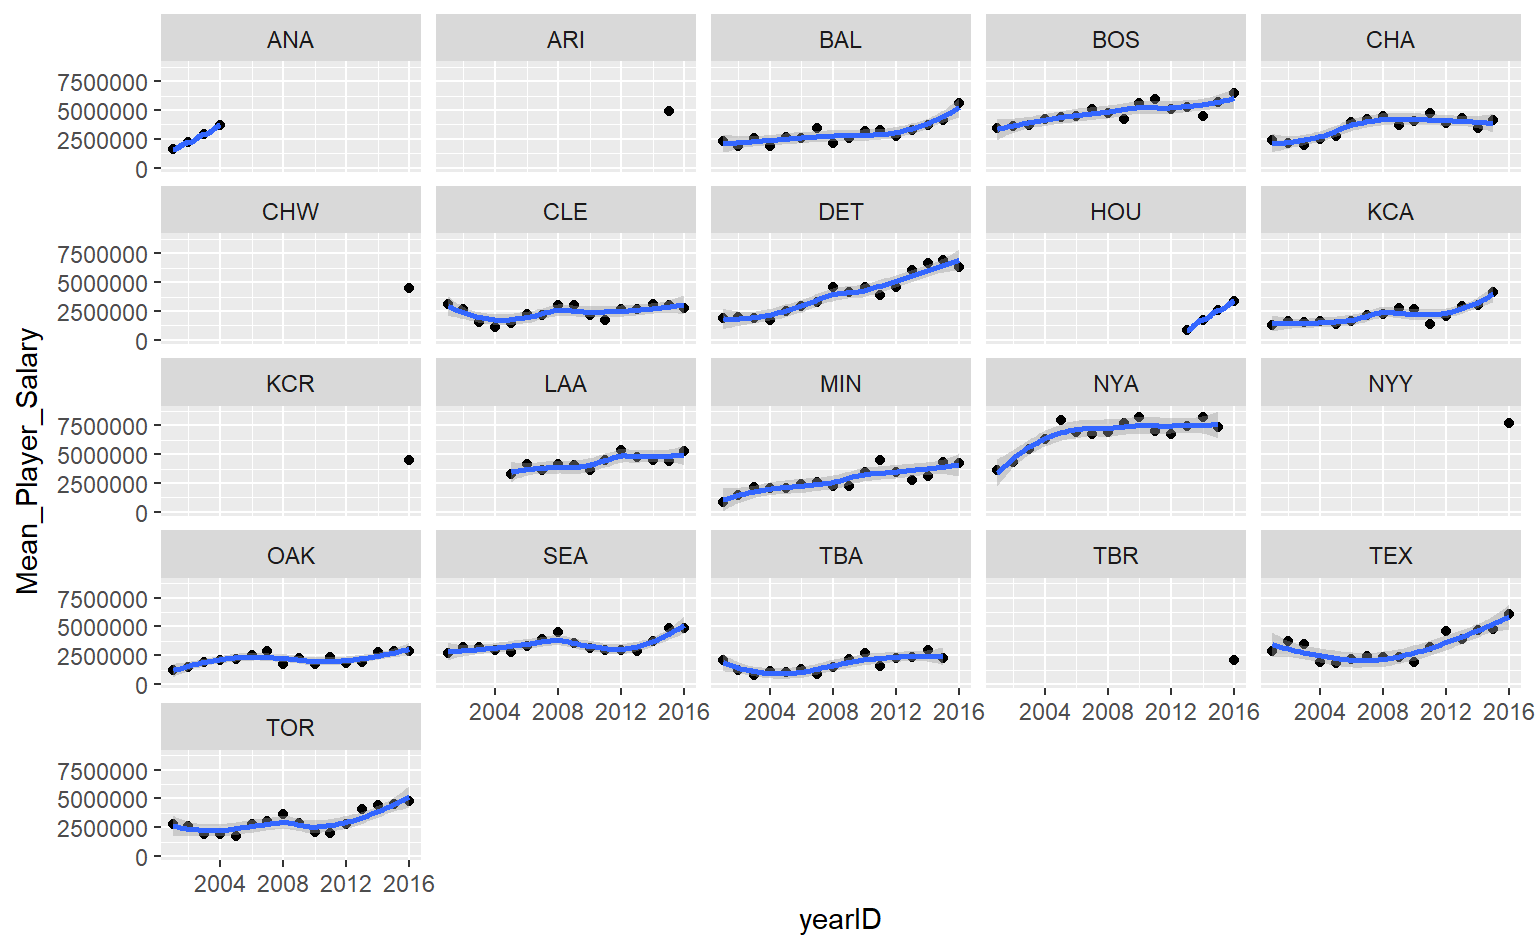
\includegraphics[width=0.7\linewidth]{DS4PS-I_files/figure-latex/unnamed-chunk-165-1} \end{center}

Now you can quickly see that Detroit is the team that has raised
salaries most aggressively.

If we need to, we can easily convert a tidy dataset into something that
looks like a table using the \textbf{spread()} function:

\begin{Shaded}
\begin{Highlighting}[]

\NormalTok{Salaries }\OperatorTok\StringTok{ }\KeywordTok{filter}\NormalTok{( yearID }\OperatorTok{>}\StringTok{ }\DecValTok{2006} \OperatorTok{&}\StringTok{ }\NormalTok{lgID }\OperatorTok{==}\StringTok{ "NL"}\NormalTok{ ) }\OperatorTok\StringTok{ }
\StringTok{             }\KeywordTok{group_by}\NormalTok{( teamID, yearID ) }\OperatorTok\StringTok{ }
\StringTok{             }\KeywordTok{summarize}\NormalTok{( }\DataTypeTok{mean =} \KeywordTok{dollar}\NormalTok{(}\KeywordTok{mean}\NormalTok{(salary)) ) }\OperatorTok
\StringTok{             }\KeywordTok{spread}\NormalTok{( }\DataTypeTok{key=}\NormalTok{yearID, }\DataTypeTok{value=}\NormalTok{mean, }\DataTypeTok{sep=}\StringTok{"_"}\NormalTok{ ) }\OperatorTok\StringTok{ }
\StringTok{             }\KeywordTok{select}\NormalTok{( }\DecValTok{1}\OperatorTok{:}\DecValTok{6}\NormalTok{ ) }\OperatorTok\StringTok{ }\KeywordTok{na.omit}\NormalTok{() }\OperatorTok
\StringTok{             }\NormalTok{pander}
\end{Highlighting}
\end{Shaded}

\begin{longtable}[]{@{}cccccc@{}}
\toprule
\begin{minipage}[b]{0.09\columnwidth}\centering
teamID\strut
\end{minipage} & \begin{minipage}[b]{0.15\columnwidth}\centering
yearID\_2007\strut
\end{minipage} & \begin{minipage}[b]{0.15\columnwidth}\centering
yearID\_2008\strut
\end{minipage} & \begin{minipage}[b]{0.15\columnwidth}\centering
yearID\_2009\strut
\end{minipage} & \begin{minipage}[b]{0.15\columnwidth}\centering
yearID\_2010\strut
\end{minipage} & \begin{minipage}[b]{0.15\columnwidth}\centering
yearID\_2011\strut
\end{minipage}\tabularnewline
\midrule
\endhead
\begin{minipage}[t]{0.09\columnwidth}\centering
ARI\strut
\end{minipage} & \begin{minipage}[t]{0.15\columnwidth}\centering
\$1,859,555\strut
\end{minipage} & \begin{minipage}[t]{0.15\columnwidth}\centering
\$2,364,383\strut
\end{minipage} & \begin{minipage}[t]{0.15\columnwidth}\centering
\$2,812,141\strut
\end{minipage} & \begin{minipage}[t]{0.15\columnwidth}\centering
\$2,335,314\strut
\end{minipage} & \begin{minipage}[t]{0.15\columnwidth}\centering
\$1,986,660\strut
\end{minipage}\tabularnewline
\begin{minipage}[t]{0.09\columnwidth}\centering
ATL\strut
\end{minipage} & \begin{minipage}[t]{0.15\columnwidth}\centering
\$3,117,530\strut
\end{minipage} & \begin{minipage}[t]{0.15\columnwidth}\centering
\$3,412,189\strut
\end{minipage} & \begin{minipage}[t]{0.15\columnwidth}\centering
\$3,335,385\strut
\end{minipage} & \begin{minipage}[t]{0.15\columnwidth}\centering
\$3,126,802\strut
\end{minipage} & \begin{minipage}[t]{0.15\columnwidth}\centering
\$3,346,257\strut
\end{minipage}\tabularnewline
\begin{minipage}[t]{0.09\columnwidth}\centering
CHN\strut
\end{minipage} & \begin{minipage}[t]{0.15\columnwidth}\centering
\$3,691,494\strut
\end{minipage} & \begin{minipage}[t]{0.15\columnwidth}\centering
\$4,383,179\strut
\end{minipage} & \begin{minipage}[t]{0.15\columnwidth}\centering
\$5,392,360\strut
\end{minipage} & \begin{minipage}[t]{0.15\columnwidth}\centering
\$5,429,963\strut
\end{minipage} & \begin{minipage}[t]{0.15\columnwidth}\centering
\$5,001,893\strut
\end{minipage}\tabularnewline
\begin{minipage}[t]{0.09\columnwidth}\centering
CIN\strut
\end{minipage} & \begin{minipage}[t]{0.15\columnwidth}\centering
\$2,210,483\strut
\end{minipage} & \begin{minipage}[t]{0.15\columnwidth}\centering
\$2,647,061\strut
\end{minipage} & \begin{minipage}[t]{0.15\columnwidth}\centering
\$3,198,196\strut
\end{minipage} & \begin{minipage}[t]{0.15\columnwidth}\centering
\$2,760,059\strut
\end{minipage} & \begin{minipage}[t]{0.15\columnwidth}\centering
\$2,531,571\strut
\end{minipage}\tabularnewline
\begin{minipage}[t]{0.09\columnwidth}\centering
COL\strut
\end{minipage} & \begin{minipage}[t]{0.15\columnwidth}\centering
\$2,078,500\strut
\end{minipage} & \begin{minipage}[t]{0.15\columnwidth}\centering
\$2,640,596\strut
\end{minipage} & \begin{minipage}[t]{0.15\columnwidth}\centering
\$2,785,222\strut
\end{minipage} & \begin{minipage}[t]{0.15\columnwidth}\centering
\$2,904,379\strut
\end{minipage} & \begin{minipage}[t]{0.15\columnwidth}\centering
\$3,390,310\strut
\end{minipage}\tabularnewline
\begin{minipage}[t]{0.09\columnwidth}\centering
FLO\strut
\end{minipage} & \begin{minipage}[t]{0.15\columnwidth}\centering
\$984,097\strut
\end{minipage} & \begin{minipage}[t]{0.15\columnwidth}\centering
\$660,955\strut
\end{minipage} & \begin{minipage}[t]{0.15\columnwidth}\centering
\$1,315,500\strut
\end{minipage} & \begin{minipage}[t]{0.15\columnwidth}\centering
\$2,112,212\strut
\end{minipage} & \begin{minipage}[t]{0.15\columnwidth}\centering
\$2,190,154\strut
\end{minipage}\tabularnewline
\begin{minipage}[t]{0.09\columnwidth}\centering
HOU\strut
\end{minipage} & \begin{minipage}[t]{0.15\columnwidth}\centering
\$3,250,333\strut
\end{minipage} & \begin{minipage}[t]{0.15\columnwidth}\centering
\$3,293,719\strut
\end{minipage} & \begin{minipage}[t]{0.15\columnwidth}\centering
\$3,814,682\strut
\end{minipage} & \begin{minipage}[t]{0.15\columnwidth}\centering
\$3,298,411\strut
\end{minipage} & \begin{minipage}[t]{0.15\columnwidth}\centering
\$2,437,724\strut
\end{minipage}\tabularnewline
\begin{minipage}[t]{0.09\columnwidth}\centering
LAN\strut
\end{minipage} & \begin{minipage}[t]{0.15\columnwidth}\centering
\$3,739,811\strut
\end{minipage} & \begin{minipage}[t]{0.15\columnwidth}\centering
\$4,089,260\strut
\end{minipage} & \begin{minipage}[t]{0.15\columnwidth}\centering
\$4,016,584\strut
\end{minipage} & \begin{minipage}[t]{0.15\columnwidth}\centering
\$3,531,778\strut
\end{minipage} & \begin{minipage}[t]{0.15\columnwidth}\centering
\$3,472,967\strut
\end{minipage}\tabularnewline
\begin{minipage}[t]{0.09\columnwidth}\centering
MIL\strut
\end{minipage} & \begin{minipage}[t]{0.15\columnwidth}\centering
\$2,629,130\strut
\end{minipage} & \begin{minipage}[t]{0.15\columnwidth}\centering
\$2,790,948\strut
\end{minipage} & \begin{minipage}[t]{0.15\columnwidth}\centering
\$3,083,942\strut
\end{minipage} & \begin{minipage}[t]{0.15\columnwidth}\centering
\$2,796,837\strut
\end{minipage} & \begin{minipage}[t]{0.15\columnwidth}\centering
\$2,849,911\strut
\end{minipage}\tabularnewline
\begin{minipage}[t]{0.09\columnwidth}\centering
NYN\strut
\end{minipage} & \begin{minipage}[t]{0.15\columnwidth}\centering
\$3,841,055\strut
\end{minipage} & \begin{minipage}[t]{0.15\columnwidth}\centering
\$4,593,113\strut
\end{minipage} & \begin{minipage}[t]{0.15\columnwidth}\centering
\$5,334,785\strut
\end{minipage} & \begin{minipage}[t]{0.15\columnwidth}\centering
\$4,800,819\strut
\end{minipage} & \begin{minipage}[t]{0.15\columnwidth}\centering
\$4,401,752\strut
\end{minipage}\tabularnewline
\begin{minipage}[t]{0.09\columnwidth}\centering
PHI\strut
\end{minipage} & \begin{minipage}[t]{0.15\columnwidth}\centering
\$2,980,940\strut
\end{minipage} & \begin{minipage}[t]{0.15\columnwidth}\centering
\$3,495,710\strut
\end{minipage} & \begin{minipage}[t]{0.15\columnwidth}\centering
\$4,185,335\strut
\end{minipage} & \begin{minipage}[t]{0.15\columnwidth}\centering
\$5,068,871\strut
\end{minipage} & \begin{minipage}[t]{0.15\columnwidth}\centering
\$5,765,879\strut
\end{minipage}\tabularnewline
\begin{minipage}[t]{0.09\columnwidth}\centering
PIT\strut
\end{minipage} & \begin{minipage}[t]{0.15\columnwidth}\centering
\$1,427,327\strut
\end{minipage} & \begin{minipage}[t]{0.15\columnwidth}\centering
\$1,872,684\strut
\end{minipage} & \begin{minipage}[t]{0.15\columnwidth}\centering
\$1,872,808\strut
\end{minipage} & \begin{minipage}[t]{0.15\columnwidth}\centering
\$1,294,185\strut
\end{minipage} & \begin{minipage}[t]{0.15\columnwidth}\centering
\$1,553,345\strut
\end{minipage}\tabularnewline
\begin{minipage}[t]{0.09\columnwidth}\centering
SDN\strut
\end{minipage} & \begin{minipage}[t]{0.15\columnwidth}\centering
\$2,235,022\strut
\end{minipage} & \begin{minipage}[t]{0.15\columnwidth}\centering
\$2,376,697\strut
\end{minipage} & \begin{minipage}[t]{0.15\columnwidth}\centering
\$1,604,952\strut
\end{minipage} & \begin{minipage}[t]{0.15\columnwidth}\centering
\$1,453,819\strut
\end{minipage} & \begin{minipage}[t]{0.15\columnwidth}\centering
\$1,479,650\strut
\end{minipage}\tabularnewline
\begin{minipage}[t]{0.09\columnwidth}\centering
SFN\strut
\end{minipage} & \begin{minipage}[t]{0.15\columnwidth}\centering
\$3,469,964\strut
\end{minipage} & \begin{minipage}[t]{0.15\columnwidth}\centering
\$2,641,190\strut
\end{minipage} & \begin{minipage}[t]{0.15\columnwidth}\centering
\$2,965,230\strut
\end{minipage} & \begin{minipage}[t]{0.15\columnwidth}\centering
\$3,522,905\strut
\end{minipage} & \begin{minipage}[t]{0.15\columnwidth}\centering
\$4,377,716\strut
\end{minipage}\tabularnewline
\begin{minipage}[t]{0.09\columnwidth}\centering
SLN\strut
\end{minipage} & \begin{minipage}[t]{0.15\columnwidth}\centering
\$3,224,529\strut
\end{minipage} & \begin{minipage}[t]{0.15\columnwidth}\centering
\$3,018,923\strut
\end{minipage} & \begin{minipage}[t]{0.15\columnwidth}\centering
\$3,278,830\strut
\end{minipage} & \begin{minipage}[t]{0.15\columnwidth}\centering
\$3,741,630\strut
\end{minipage} & \begin{minipage}[t]{0.15\columnwidth}\centering
\$3,904,947\strut
\end{minipage}\tabularnewline
\begin{minipage}[t]{0.09\columnwidth}\centering
WAS\strut
\end{minipage} & \begin{minipage}[t]{0.15\columnwidth}\centering
\$1,319,554\strut
\end{minipage} & \begin{minipage}[t]{0.15\columnwidth}\centering
\$1,895,207\strut
\end{minipage} & \begin{minipage}[t]{0.15\columnwidth}\centering
\$2,140,286\strut
\end{minipage} & \begin{minipage}[t]{0.15\columnwidth}\centering
\$2,046,667\strut
\end{minipage} & \begin{minipage}[t]{0.15\columnwidth}\centering
\$2,201,963\strut
\end{minipage}\tabularnewline
\bottomrule
\end{longtable}

\begin{Shaded}
\begin{Highlighting}[]


\NormalTok{Salaries }\OperatorTok\StringTok{ }\KeywordTok{filter}\NormalTok{( yearID }\OperatorTok{>}\StringTok{ }\DecValTok{2006} \OperatorTok{&}\StringTok{ }\NormalTok{lgID }\OperatorTok{==}\StringTok{ "NL"}\NormalTok{ ) }\OperatorTok\StringTok{ }
\StringTok{             }\KeywordTok{group_by}\NormalTok{( teamID, yearID ) }\OperatorTok\StringTok{ }
\StringTok{             }\KeywordTok{summarize}\NormalTok{( }\DataTypeTok{mean =} \KeywordTok{dollar}\NormalTok{(}\KeywordTok{mean}\NormalTok{(salary)) ) }\OperatorTok
\StringTok{             }\KeywordTok{spread}\NormalTok{( }\DataTypeTok{key=}\NormalTok{teamID, }\DataTypeTok{value=}\NormalTok{mean, }\DataTypeTok{sep=}\StringTok{"_"}\NormalTok{ ) }\OperatorTok\StringTok{ }
\StringTok{             }\KeywordTok{select}\NormalTok{( }\DecValTok{1}\OperatorTok{:}\DecValTok{6}\NormalTok{ ) }\OperatorTok\StringTok{ }
\StringTok{             }\NormalTok{pander}
\end{Highlighting}
\end{Shaded}

\begin{longtable}[]{@{}cccccc@{}}
\toprule
\begin{minipage}[b]{0.10\columnwidth}\centering
yearID\strut
\end{minipage} & \begin{minipage}[b]{0.15\columnwidth}\centering
teamID\_ARI\strut
\end{minipage} & \begin{minipage}[b]{0.15\columnwidth}\centering
teamID\_ATL\strut
\end{minipage} & \begin{minipage}[b]{0.15\columnwidth}\centering
teamID\_CHC\strut
\end{minipage} & \begin{minipage}[b]{0.15\columnwidth}\centering
teamID\_CHN\strut
\end{minipage} & \begin{minipage}[b]{0.15\columnwidth}\centering
teamID\_CIN\strut
\end{minipage}\tabularnewline
\midrule
\endhead
\begin{minipage}[t]{0.10\columnwidth}\centering
2007\strut
\end{minipage} & \begin{minipage}[t]{0.15\columnwidth}\centering
\$1,859,555\strut
\end{minipage} & \begin{minipage}[t]{0.15\columnwidth}\centering
\$3,117,530\strut
\end{minipage} & \begin{minipage}[t]{0.15\columnwidth}\centering
NA\strut
\end{minipage} & \begin{minipage}[t]{0.15\columnwidth}\centering
\$3,691,494\strut
\end{minipage} & \begin{minipage}[t]{0.15\columnwidth}\centering
\$2,210,483\strut
\end{minipage}\tabularnewline
\begin{minipage}[t]{0.10\columnwidth}\centering
2008\strut
\end{minipage} & \begin{minipage}[t]{0.15\columnwidth}\centering
\$2,364,383\strut
\end{minipage} & \begin{minipage}[t]{0.15\columnwidth}\centering
\$3,412,189\strut
\end{minipage} & \begin{minipage}[t]{0.15\columnwidth}\centering
NA\strut
\end{minipage} & \begin{minipage}[t]{0.15\columnwidth}\centering
\$4,383,179\strut
\end{minipage} & \begin{minipage}[t]{0.15\columnwidth}\centering
\$2,647,061\strut
\end{minipage}\tabularnewline
\begin{minipage}[t]{0.10\columnwidth}\centering
2009\strut
\end{minipage} & \begin{minipage}[t]{0.15\columnwidth}\centering
\$2,812,141\strut
\end{minipage} & \begin{minipage}[t]{0.15\columnwidth}\centering
\$3,335,385\strut
\end{minipage} & \begin{minipage}[t]{0.15\columnwidth}\centering
NA\strut
\end{minipage} & \begin{minipage}[t]{0.15\columnwidth}\centering
\$5,392,360\strut
\end{minipage} & \begin{minipage}[t]{0.15\columnwidth}\centering
\$3,198,196\strut
\end{minipage}\tabularnewline
\begin{minipage}[t]{0.10\columnwidth}\centering
2010\strut
\end{minipage} & \begin{minipage}[t]{0.15\columnwidth}\centering
\$2,335,314\strut
\end{minipage} & \begin{minipage}[t]{0.15\columnwidth}\centering
\$3,126,802\strut
\end{minipage} & \begin{minipage}[t]{0.15\columnwidth}\centering
NA\strut
\end{minipage} & \begin{minipage}[t]{0.15\columnwidth}\centering
\$5,429,963\strut
\end{minipage} & \begin{minipage}[t]{0.15\columnwidth}\centering
\$2,760,059\strut
\end{minipage}\tabularnewline
\begin{minipage}[t]{0.10\columnwidth}\centering
2011\strut
\end{minipage} & \begin{minipage}[t]{0.15\columnwidth}\centering
\$1,986,660\strut
\end{minipage} & \begin{minipage}[t]{0.15\columnwidth}\centering
\$3,346,257\strut
\end{minipage} & \begin{minipage}[t]{0.15\columnwidth}\centering
NA\strut
\end{minipage} & \begin{minipage}[t]{0.15\columnwidth}\centering
\$5,001,893\strut
\end{minipage} & \begin{minipage}[t]{0.15\columnwidth}\centering
\$2,531,571\strut
\end{minipage}\tabularnewline
\begin{minipage}[t]{0.10\columnwidth}\centering
2012\strut
\end{minipage} & \begin{minipage}[t]{0.15\columnwidth}\centering
\$2,733,512\strut
\end{minipage} & \begin{minipage}[t]{0.15\columnwidth}\centering
\$2,856,205\strut
\end{minipage} & \begin{minipage}[t]{0.15\columnwidth}\centering
NA\strut
\end{minipage} & \begin{minipage}[t]{0.15\columnwidth}\centering
\$3,392,194\strut
\end{minipage} & \begin{minipage}[t]{0.15\columnwidth}\centering
\$2,935,843\strut
\end{minipage}\tabularnewline
\begin{minipage}[t]{0.10\columnwidth}\centering
2013\strut
\end{minipage} & \begin{minipage}[t]{0.15\columnwidth}\centering
\$3,004,400\strut
\end{minipage} & \begin{minipage}[t]{0.15\columnwidth}\centering
\$3,254,501\strut
\end{minipage} & \begin{minipage}[t]{0.15\columnwidth}\centering
NA\strut
\end{minipage} & \begin{minipage}[t]{0.15\columnwidth}\centering
\$3,867,989\strut
\end{minipage} & \begin{minipage}[t]{0.15\columnwidth}\centering
\$4,256,178\strut
\end{minipage}\tabularnewline
\begin{minipage}[t]{0.10\columnwidth}\centering
2014\strut
\end{minipage} & \begin{minipage}[t]{0.15\columnwidth}\centering
\$3,763,904\strut
\end{minipage} & \begin{minipage}[t]{0.15\columnwidth}\centering
\$4,067,042\strut
\end{minipage} & \begin{minipage}[t]{0.15\columnwidth}\centering
NA\strut
\end{minipage} & \begin{minipage}[t]{0.15\columnwidth}\centering
\$2,426,759\strut
\end{minipage} & \begin{minipage}[t]{0.15\columnwidth}\centering
\$3,864,911\strut
\end{minipage}\tabularnewline
\begin{minipage}[t]{0.10\columnwidth}\centering
2015\strut
\end{minipage} & \begin{minipage}[t]{0.15\columnwidth}\centering
\$2,034,250\strut
\end{minipage} & \begin{minipage}[t]{0.15\columnwidth}\centering
\$2,990,885\strut
\end{minipage} & \begin{minipage}[t]{0.15\columnwidth}\centering
NA\strut
\end{minipage} & \begin{minipage}[t]{0.15\columnwidth}\centering
\$4,138,547\strut
\end{minipage} & \begin{minipage}[t]{0.15\columnwidth}\centering
\$4,187,862\strut
\end{minipage}\tabularnewline
\begin{minipage}[t]{0.10\columnwidth}\centering
2016\strut
\end{minipage} & \begin{minipage}[t]{0.15\columnwidth}\centering
\$3,363,041\strut
\end{minipage} & \begin{minipage}[t]{0.15\columnwidth}\centering
\$2,362,010\strut
\end{minipage} & \begin{minipage}[t]{0.15\columnwidth}\centering
\$5,312,678\strut
\end{minipage} & \begin{minipage}[t]{0.15\columnwidth}\centering
NA\strut
\end{minipage} & \begin{minipage}[t]{0.15\columnwidth}\centering
\$3,066,899\strut
\end{minipage}\tabularnewline
\bottomrule
\end{longtable}

\bibliography{book.bib,packages.bib}


\end{document}
